\PassOptionsToPackage{hyphens}{url}
\documentclass[11pt,reqno]{amsart}
\usepackage[margin=1in]{geometry}
\usepackage{amsmath,amssymb,amsthm,mathtools}
\usepackage{booktabs}
\usepackage{longtable}
\usepackage{microtype}
\usepackage{enumitem}
\usepackage{pgfplots}
\pgfplotsset{compat=1.17}
\usetikzlibrary{positioning,arrows.meta}
\usepackage[colorlinks=true,linkcolor=blue,citecolor=blue,urlcolor=blue]{hyperref}

\theoremstyle{plain}
\newtheorem{theorem}{Theorem}[section]
\newtheorem{proposition}[theorem]{Proposition}
\newtheorem{corollary}[theorem]{Corollary}
\newtheorem{lemma}[theorem]{Lemma}
\newtheorem{conjecture}[theorem]{Conjecture}
\newtheorem{claim}[theorem]{Claim}
\theoremstyle{definition}
\newtheorem{definition}[theorem]{Definition}
\newtheorem{example}[theorem]{Example}
\newtheorem{protocol}[theorem]{Protocol}
\theoremstyle{remark}
\newtheorem{remark}[theorem]{Remark}

\newcommand{\R}{\mathbb{R}}
\newcommand{\N}{\mathbb{N}}
\newcommand{\Z}{\mathbb{Z}}
\newcommand{\PP}{\mathbb{P}}
\newcommand{\EE}{\mathbb{E}}
\newcommand{\eps}{\varepsilon}
\newcommand{\Store}{\mathfrak{S}}
\newcommand{\Kinds}{\mathcal{K}}
\newcommand{\cV}{\mathcal{V}}
\newcommand{\cE}{\mathcal{E}}
\newcommand{\cL}{\mathcal{L}}
\newcommand{\cQ}{\mathcal{Q}}
\newcommand{\cP}{\mathcal{P}}
\newcommand{\cH}{\mathcal{H}}
\newcommand{\cR}{\mathcal{R}}
\newcommand{\tool}[1]{\texttt{#1}}
\DeclareMathOperator{\Var}{Var}
\DeclareMathOperator{\Inf}{Inf}
\DeclareMathOperator{\idf}{idf}
\DeclareMathOperator{\BM}{BM25}
\DeclareMathOperator{\str}{str}
\DeclareMathOperator{\simil}{sim}
\DeclareMathOperator{\KL}{D}

% hyperlinked statement/proof cross-references
\newcommand{\proofbutton}[1]{\hyperref[proof:#1]{\textnormal{\footnotesize\textsf{[proof $\to$]}}}}
\newcommand{\stmtbutton}[1]{\hyperref[#1]{\textnormal{\footnotesize\textsf{[$\leftarrow$ statement]}}}}

\title[Shared memory for multi-agent mathematical research]{Math Brain: Shared, Auditable Memory for Multi-Agent Mathematical Research}
\author{Yitzchak Shmalo}
\address{Einstein Institute of Mathematics, The Hebrew University of Jerusalem, Givat Ram, Jerusalem, Israel}
\email{yitzchak.shmalo@gmail.com}
\date{October 22, 2026}
\subjclass[2020]{Primary 68T05, 68T20; Secondary 68P20, 03B35, 42C10, 60K35}
\keywords{AI for mathematics, agent memory, retrieval, knowledge graphs, Hebbian learning, BM25, paired evaluation, McNemar test, Fourier entropy-influence conjecture, Ising perceptron}
\hypersetup{
  pdftitle={Math Brain: Shared, Auditable Memory for Multi-Agent Mathematical Research},
  pdfauthor={Yitzchak Shmalo},
  pdfkeywords={AI for mathematics, agent memory, retrieval, knowledge graph, paired evaluation, Fourier entropy-influence}
}

\emergencystretch=3em
\begin{document}

\begin{abstract}
Language-model agents now do a good deal of research mathematics, but what one session establishes is lost to the next: a counterexample found at noon is unknown to the agent that takes up the same problem at one o'clock, and corrected statements and failed routes vanish with the session that found them. We describe Math Brain, a shared memory built to keep them. It is a store of mathematical cards (definitions, theorems with their exact hypotheses, sources, and the agents' own proofs, counterexamples, computations and corrected statements) joined by typed links; on 22 October 2026 it held $13{,}306$ cards and $19{,}362$ links, $231$ of them retracted and kept in the record. Agents reach it through a hook that serves a few cards on each prompt and stays silent on weak matches, a recall tool that prints whole cards with their identifiers and links, link strengths that grow with joint use, and a write-back gate that lands a packet of new cards only when a held-out recall test shows that it costs no answer. We give the structure and the ranking in full and prove the invariants on which safe sharing rests: append-only revision, order-independent bundle digests, acyclic supersession and dependency closure, and the separation of association from evidence.

In paired tests with the same model, budget and questions, the memory supplied what the agents could not otherwise know. On $1{,}000$ items whose answers are cards in the store, scores rose from $538$ to $1{,}000$, with no harm observed. On a second bank of $1{,}000$ items run in three arms, the brain, the research repositories without the brain, and the model alone, Claude agents scored $94.3\%$, $78.1\%$ and $21.7\%$ on the $755$ items run in all three arms; on the items that the first two arms both finished in time they scored the same ($99.2\%$ and $99.3\%$), so the brain's lead over the repositories is time, and it came at a quarter of the input and under three fifths of the session time and price. Codex agents, given more time, scored $93.4\%$ with the brain and $97.3\%$ with the repositories ($p=0.09$). On $100$ questions about results held in the store, agents scored $0$ with no tools, $75$ with text search and $83$ with the recall tool, and adding the hook and the link walk gave $82$ while cutting uncached input by a factor of $1.8$. A ranking change raised held-out hits from $298$ to $317$ of $584$ (exact McNemar $p=0.0019$). On $61$ reasoning and audit items the full package, which also adds a clock and a hint, beat tools alone $52$ to $41$ ($p=0.019$, not significant after correction for the paper's nineteen comparisons). We report the nulls and losses with the same care: no significant gain over agents given the documents and a recall tool, none on thirteen new open problems, and a significant loss by an early version to agents given the documents, on $300$ hard items. The question banks are private, so every test can be repeated on later versions.

The paper also records mathematics from the same program, including a reduction of the Fourier entropy-influence conjecture: for every Boolean function $H(f)\le 2(I(f)-\Var f)+2U(f)$, where $U$ compares each Fourier weight with the weight above it, so the conjecture is equivalent to $\sup U/I<\infty$. We prove this and a summed restriction criterion that would give the conjecture with an explicit constant.
\end{abstract}

\maketitle

\setcounter{tocdepth}{1}
\tableofcontents

\section{Introduction}\label{sec:intro}

A language-model agent working on a mathematical problem is, in one respect, a very strange collaborator: it forgets everything when its session ends. It may have spent three hours establishing that a natural route to a conjecture fails, with an explicit counterexample checked to sixty digits, and the next agent asked about the same conjecture will walk into the same route the next morning. The waste is larger when many agents work at once. In the work reported here, up to a hundred agents worked one conjecture in parallel, and several hundred scheduled tasks ran around the clock on a list of four hundred open problems; without a common memory, each of them would rediscover the same definitions, the same failed reductions and the same known counterexamples, and none could build on what another had settled an hour before.

Math Brain is a shared memory built to remove that limitation. It is a store of short mathematical records, which we call \emph{cards}, joined by typed \emph{links}, together with the tools agents use to search it, to move along its links and to write back to it while they work. The cards are of the kinds a mathematician keeps in a notebook: definitions, theorems with their exact hypotheses, proof techniques, sources, conjectures, and, most importantly, the agents' own results: proofs, counterexamples, verified computations, refuted routes and corrected statements. The links say how two cards relate. One result depends on another, generalizes it, specializes it, is analogous to it, cites it, refutes it, or fails under its hypotheses. On 22 October 2026 the store held $13{,}306$ cards and $19{,}362$ links, $231$ of them retracted and kept in the record, and it had grown from $800$ cards on 2 August.

The agents that use the brain are the agents that build it. An agent reads the store before it works and writes to it when it finds something; the next agent then starts where the previous one stopped. Below we set out that loop in full, measure what it does for an agent, and record the mathematics that came out of the work.

\subsection{The loop}

The memory is surrounded by five mechanisms; each is treated in its own section.

\begin{enumerate}[label=(\roman*)]
\item \emph{Served cards} (Section~\ref{sec:hook}). A hook runs on every prompt an agent receives, in both of the agent runtimes we used, and places a few cards in front of the agent, each with a line saying how far to trust it. When nothing in the store matches well, the hook stays silent.
\item \emph{Deliberate recall} (Section~\ref{sec:retrieval}). When an agent needs something, it searches the store and receives whole cards, with their identifiers and the identifiers of their links. From any card it can step along the links.
\item \emph{Links that grow with use} (Section~\ref{sec:strength}). When an agent uses two cards together, the link between them strengthens; strengths fade by a power law, so the links agents actually rely on are printed first and weigh more in a walk.
\item \emph{Writing back} (Section~\ref{sec:writeback}). An agent writes its results as a sealed \emph{packet} of new cards and links with their sources. Before a packet lands, a held-out recall test is run on a copy of the store with the packet added, and a packet that costs an answer is held back. Wrong cards are never deleted; a corrected revision supersedes them and the supersession is recorded.
\item \emph{Shared work orders} (Section~\ref{sec:collective}). Scheduled agents read a common board and a common work order and commit their reports to a shared repository, from which their results enter the store through the same gate.
\end{enumerate}
Figure~\ref{fig:arch} shows how the parts fit together.

\begin{figure}[ht]
\centering
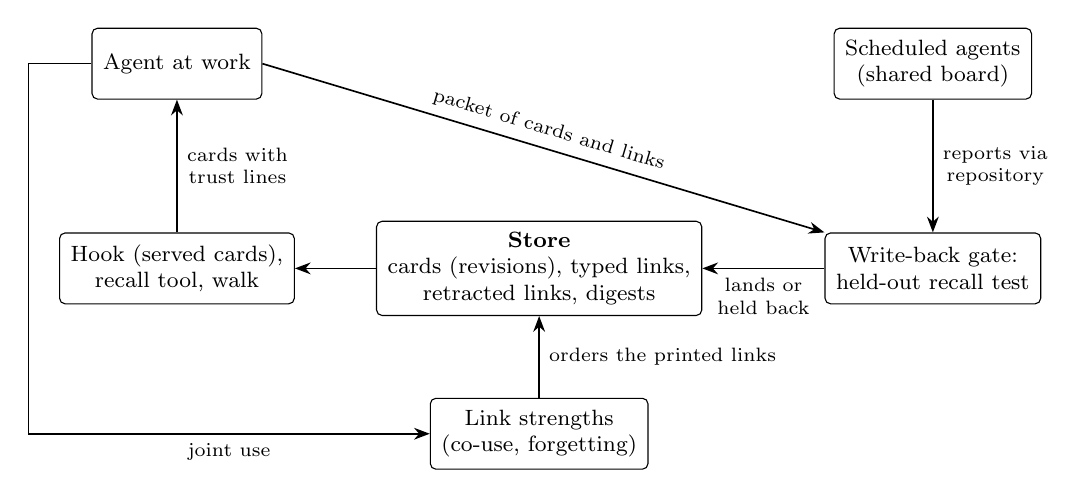
\begin{tikzpicture}[
  box/.style={draw, rounded corners=2pt, align=center, font=\footnotesize, minimum height=0.9cm, inner sep=4pt},
  arr/.style={-{Stealth[length=2mm]}, semithick},
  lab/.style={font=\scriptsize, align=center}]
\node[box, minimum width=4.0cm] (store) at (4,0) {\textbf{Store}\\ cards (revisions), typed links,\\ retracted links, digests};
\node[box] (read) at (-0.6,0) {Hook (served cards),\\ recall tool, walk};
\node[box] (gate) at (9.0,0) {Write-back gate:\\ held-out recall test};
\node[box] (agent) at (-0.6,2.6) {Agent at work};
\node[box] (sched) at (9.0,2.6) {Scheduled agents\\ (shared board)};
\node[box] (str) at (4,-2.1) {Link strengths\\ (co-use, forgetting)};
\draw[arr] (store) -- (read);
\draw[arr] (read) -- node[lab, right] {cards with\\ trust lines} (agent);
\draw[arr] (agent.east) -- node[lab, above, sloped] {packet of cards and links} (gate.north west);
\draw[arr] (sched) -- node[lab, right] {reports via\\ repository} (gate);
\draw[arr] (gate) -- node[lab, below] {lands or\\ held back} (store);
\draw[arr] (agent.west) -- ++(-0.8,0) |- node[lab, pos=0.75, below] {joint use} (str.west);
\draw[arr] (str) -- node[lab, right] {orders the printed links} (store);
\end{tikzpicture}
\caption{The loop. Agents read the store through the hook, the recall tool and the walk, and write to it only through the gate, which lands a packet of new cards and links when a held-out recall test on a copy of the store shows that it costs no answer. Joint use of two cards strengthens the link between them; the strengths order the printed links and weight the walk, but cannot change which cards a search without spreading returns (Proposition~\ref{prop:strength-search}).}
\label{fig:arch}
\end{figure}


\subsection{What we measured}

Every test in this paper compares two arms that use the same model, the same budget and the same questions, and differ only in access to the brain; the one exception, a solving test whose full package also adds a clock and a hint, is marked where it occurs. Scores are counts of correct answers; $p$-values are exact two-sided McNemar tests on the items where the arms disagree. The question banks and their answer keys are kept private, so the same tests can be run on later versions of the system without the answers having been seen. Table~\ref{tab:intro-summary} collects the main comparisons; Section~\ref{sec:tests} gives each one in detail.

\begin{table}[ht]
\centering
\small
\begin{tabular}{p{6.2cm}ccc}
\toprule
Test & Without the brain & With the brain & $p$ \\
\midrule
100 questions about results held in the store (11 Oct) & 75 (text search) & 82 (full stack)$^{a}$ & 0.09 \\
1{,}000 items whose answers are cards in the store (13 Sep) & 538 & 1{,}000 & $1.7\cdot 10^{-139}$ \\
61 reasoning and audit items (5--6 Oct) & 41 & 52 & 0.019 \\
\quad of which, 26 items naming a known result & 13 & 22 & 0.012 \\
80 questions about files in GitHub repositories (12 Oct) & 68 & 73 & 0.27 \\
584 held-out ranking questions, before and after (12 Oct) & 298 & 317 & 0.0019 \\
13 new open problems, graded blind (11 Oct) & 26 of 39 & 24 of 39 & 0.23$^{b}$ \\
755 store items, three arms: repositories against brain, Claude (24 Oct) & $78.1\%$ & $94.3\%$ & $3.0\cdot 10^{-27}$ \\
\quad of which, 593 items both arms answered in time & $99.3\%$ & $99.2\%$ & 1 \\
182 store items, three arms: repositories against brain, Codex (24 Oct) & $97.3\%$ & $93.4\%$ & 0.09 \\
300 hard items, early version against documents & 264 & 238 & 0.0005 \\
\bottomrule
\end{tabular}
\caption{The main paired comparisons. $^{a}$The full stack is the hook, the recall tool and the link walk; it went $10$ to $3$ against text search on the disagreeing items. The recall tool alone scored $83$. $^{b}$Each attempt was graded blind at up to $3$ points, so $39$ is the maximum over $13$ problems; the $p$-value is for a referee's pairwise preference, $8$ to $3$ for the arm without the brain, with $2$ even. The last two rows are tests the brain did not pass. The three-arm rows give the percentage correct on the items run in all three arms; the model alone scored $21.7\%$ and $31.9\%$. The recall and ranking comparisons and the Claude three-arm comparisons survive a Holm correction over all nineteen paired comparisons of the current system (Appendix~\ref{app:stats}); the early version's loss survives it too.}
\label{tab:intro-summary}
\end{table}

Three findings deserve to be stated in the introduction, because they determine how the system should be used.

First, \emph{the brain helps where an answer has to be recalled, and not where it can be derived}. On the $1{,}000$ recall items the brain helped on $462$ and no harm was observed. On the $61$ reasoning items the gain lies mostly in the $26$ items that name a known result ($22$ against $13$); on the $35$ that name none the difference is small ($30$ against $28$, $p=0.73$), which bounds the effect on such items only loosely.

Second, \emph{how results are printed matters as much as how they are found}. The same retrieval engine, printing titles and $700$-character snippets without identifiers, scored $34$ of $100$; printing whole cards with their identifiers and the identifiers of their links scored $83$. Two or three wordings of a question in one search call raised the score from $76$ to $86$ of $100$ held-out questions.

Third, \emph{following links saves cost more than it adds accuracy}. On the $100$ store questions, adding the hook and the link walk to the recall tool changed accuracy by one question ($82$ against $83$, a test that could detect only a large difference), reduced the uncached input by a factor of $1.8$, and cut the session time from $666$ to $78$ minutes.

Fourth, \emph{against an agent that can read the repositories, the brain wins on time, not on knowledge}. In the three-arm test (Section~\ref{subsec:threearm}) Claude agents with the brain scored $94.3\%$ and agents with the repositories $78.1\%$, but on the $593$ items both finished within the time they were tied, $99.2\%$ against $99.3\%$. The repositories hold the same records; the brain reaches them with fewer searches, at a quarter of the input. Codex agents, with half again as much time, did slightly better with the repositories, and their losses with the brain were abstentions after a search that missed.

We also report what did not work. The hook by itself answers little ($7$ of the $100$ store questions); it was silent on $85$ of them, including all $60$ that had been reworded to share no words with their card. Spreading activation along links only re-ranks cards the words have already found. On thirteen new open problems on which the store held only a first attempt, the arm with the brain did not beat the arm without it, and an early version of the system lost, on a hard set of $300$ items, to agents that were simply given the documents.

\subsection{The structure in brief}

Section~\ref{sec:store} gives the store formally. Its records are immutable revisions of logical objects; every row carries a digest of its content and the reader refuses a row whose content no longer matches its digest; new material enters only as content-addressed bundles whose digest does not depend on the order of their entries. Three invariants make the store safe to share among many writers: the supersession relation is acyclic, so every logical object has a well-defined set of heads; an object with one head has a current revision, and an object with two is contested and has none until a review supersedes both; the exact dependency closure of a claim uses only directed \texttt{depends\_on} links and refuses cycles and missing nodes; and no association, however strong, can become evidence. We state and prove these in Section~\ref{sec:store} and Appendix~\ref{app:proofs}.

Section~\ref{sec:retrieval} gives the ranking. Cards are ranked by BM25 \cite{RobertsonZaragoza2009} with length normalization $b=0.4$, $k_1=1.2$, title words counted twice, and a channel of sentence embeddings; several wordings are merged by best rank. The decision to print the answering card in full, with its links, is part of the design and is measured. Section~\ref{sec:strength} gives the strength of a link as an explicit function of co-use with power-law forgetting, a hub discount and a similarity factor, and shows that the strengths cannot change which cards a search returns.

\subsection{The mathematics}

The memory was built for research, and it was used for research while it was built. Section~\ref{sec:math} describes the results, separating what is proved, what is computer-verified, and what is evidence. Two of them are proved in this paper.

\begin{theorem}[Granularity bound]\label{thm:intro-G}
For every Boolean function $f:\{-1,1\}^n\to\{-1,1\}$ with Fourier weights $p(S)=\hat f(S)^2$, let $\pi(S)=\sum_{T\supseteq S}p(T)$ and $U(f)=\sum_S p(S)\log_2(\pi(S)/p(S))$. Then
\[
H(f)\;\le\;2\bigl(I(f)-\Var f\bigr)+2U(f)-(1-\Var f)\log_2\frac{1}{1-\Var f}\;\le\;2I(f)+2U(f),
\]
where $H(f)$ is the Fourier entropy and $I(f)$ the total influence. In particular, the Fourier entropy-influence conjecture holds if and only if $\sup_f U(f)/I(f)<\infty$. \proofbutton{thm:intro-G}
\end{theorem}

\begin{theorem}[Summed restriction criterion]\label{thm:intro-GU}
For a coordinate $i$ let $\Delta_iU(f)=U(f)-\tfrac12\bigl(U(f_{i,+})+U(f_{i,-})\bigr)$, where $f_{i,\pm}$ are the restrictions $x_i=\pm1$, and let $G(f)=\sum_i\Delta_iU(f)$. If there are constants $a\ge0$ and $0\le b<1$ such that $G(f)\le a\,I(f)+b\,U(f)$ for every Boolean function, then every Boolean function satisfies $U(f)\le\frac{a}{1-b}I(f)$ and
\[
H(f)\le\Bigl(2+\frac{2a}{1-b}\Bigr)I(f).
\]
\proofbutton{thm:intro-GU}
\end{theorem}

The largest value of $G/I$ found in exhaustive, annealed and compositional searches is $3.2265$; if $G\le 3.2265\,I$ held in general, the conjecture would follow with constant $8.45$. Section~\ref{sec:math} also describes an interval-arithmetic verification, made in July before the store held the relevant material and therefore not evidence of its benefit, of the Krauth--M\'ezard capacity of the Ising perceptron \cite{KrauthMezard1989,DingSun2019,Huang2024}, the classes of Boolean functions on which the entropy-influence inequality was proved with explicit constants, and the thirty-one papers written in this work (Appendix~\ref{app:papers}).

\subsection{Organization}

Section~\ref{sec:related} places the system among earlier work. Sections~\ref{sec:store}--\ref{sec:collective} describe the store and the five mechanisms. Section~\ref{sec:tests} gives the tests, including those that failed, with their costs. Section~\ref{sec:campaign} gives the design of a controlled test of agents working together over time. Section~\ref{sec:math} describes the mathematics. Section~\ref{sec:usage} explains how to install the store, use the tools, write back to it, and repeat the tests with and without the brain. Section~\ref{sec:limits} states the limitations and the conditions of the public release. The proofs are in Appendix~\ref{app:proofs}; the statistics of the store are tabulated in Appendix~\ref{app:tables}; Appendix~\ref{app:tools} is a reference for the tools and Appendix~\ref{app:papers} lists the papers.

\section{Related work}\label{sec:related}

\subsection{Retrieval for language models}
Retrieval-augmented generation \cite{Lewis2020RAG} conditions a language model on passages retrieved from a corpus, and dense passage retrieval \cite{Karpukhin2020DPR} replaced sparse word matching by learned embeddings for open-domain question answering. Our ranking is closer to the older tradition: it is BM25 \cite{RobertsonZaragoza2009} with a modest embedding channel added. We found, as others have for technical text, that the sparse channel carries most of the signal on mathematical questions, which name objects, theorems and authors by words a dense model treats as near-synonyms. What our setting adds is the agent: the reader of the retrieved text is an agent that can search again, open a card by identifier and follow links, so the format of what is printed and the cost of each round become part of the retrieval problem. Section~\ref{sec:tests} measures both.

\subsection{Memory for agents}
Several systems give a language-model agent a memory that outlives its context. Generative agents \cite{Park2023Generative} keep a stream of observations and retrieve them by recency, importance and relevance; MemGPT \cite{Packer2023MemGPT} pages information between a main context and an external store; Reflexion \cite{Shinn2023Reflexion} keeps verbal summaries of failures and conditions later attempts on them; ReAct \cite{Yao2023ReAct} interleaves reasoning with tool calls, which is the mode in which our agents read the store. These memories belong to one agent, or to a small simulated society, and they hold experience in natural language. Math Brain differs in three ways. It is shared by many agents of two different runtimes working at once and over months. Its records are mathematical objects with typed relations, revision history and evidence, so a stored result can be checked, superseded or refuted rather than merely recalled. And the memory is the product of the agents' work: what one agent proves becomes, after a gate, what the next agent reads.

\subsection{Associative memory and its psychology}
The link strengths of Section~\ref{sec:strength} borrow from two older ideas. Hebb's postulate \cite{Hebb1949} that cells used together strengthen their connection is the rule we use for co-use; the spreading-activation model of semantic memory \cite{CollinsLoftus1975} is the model behind the optional link spreading of Section~\ref{sec:retrieval}. The power-law decay of a strength follows the empirical form of human forgetting \cite{WixtedEbbesen1991,AndersonSchooler1991}; Anderson and Schooler argued that this form matches the statistics of the environment, the probability that an item will be needed again given how often and how recently it was needed, and that is precisely the quantity a strength is meant to estimate. The separation between a fast store of episodes and a slow store of structured knowledge, with a replay process between them \cite{McClellandMcNaughtonOReilly1995}, describes our write-back path: episodes (agent sessions, reports) are kept, and only distilled, checked records enter the store.

\subsection{Formal mathematics}
Lean \cite{deMouraUllrich2021} and its library mathlib \cite{mathlib2020} are the main body of formalized mathematics. Math Brain is not a formal library and does not compete with one: most of its records are informal statements with proofs in prose, numerical certificates or counterexamples, and its status field distinguishes a statement checked by the Lean kernel from one reviewed by an agent or a person. When a record has a Lean proof, the store keeps the hash-pinned evidence (Section~\ref{sec:writeback}); when it does not, the store says so. A useful way to place the system is between a formal library, in which everything is certain and little is recent, and a research notebook, in which everything is recent and nothing is certain.

\subsection{The mathematics}
The Fourier entropy-influence conjecture is due to Friedgut and Kalai \cite{FriedgutKalai1996}; it is known for several classes, among them symmetric functions and read-once formulas \cite{OWZ2011,OT2013}, and the best known lower bound on the constant is due to Hod \cite{Hod2017}. The capacity of the Ising perceptron was predicted by Krauth and M\'ezard \cite{KrauthMezard1989}; the matching lower bound, conditional on a numerical hypothesis, is due to Ding and Sun \cite{DingSun2019}, and the upper bound, conditional on another, to Huang \cite{Huang2024}. Section~\ref{sec:math} explains what the agents added.

\subsection{Evaluation}
Every comparison in this paper is paired: both arms answer the same items, and the test statistic depends only on the items where they disagree. For binary outcomes this is McNemar's test \cite{McNemar1947}, which we use in its exact form (a two-sided binomial test with success probability $1/2$ on the disagreeing items). Paired designs remove the variance due to item difficulty, which in our banks is far larger than the effect of the brain.

\section{The store}\label{sec:store}

We treat the store as a mathematical object: a record, a link, the way new material enters, and the invariants that make it safe for many agents to write to at once. The implementation is a single SQLite database with an immutable object store beside it; we mention it only where it matters.

\subsection{Records and revisions}

\begin{definition}[Record]\label{def:record}
A \emph{record} is a tuple $r=(\lambda,\kappa,\sigma,\tau,\mu)$, where $\lambda$ is a \emph{logical identifier}, $\kappa$ a \emph{kind}, $\sigma$ a \emph{statement} (a UTF-8 text, possibly with formulas), $\tau\in\mathcal{T}$ a \emph{truth status}, and $\mu$ a finite map of metadata (title, domain, conditions, proof text, source, evidence identifiers, trust class). The \emph{revision identifier} of $r$ is $\rho(r)=h(\mathrm{canon}(r))$, where $h$ is SHA-256 and $\mathrm{canon}$ is a fixed canonical serialization (sorted keys, UTF-8 encoding, no insignificant whitespace).
\end{definition}

The kinds of nodes in the store are claims, sources, evidence and external references; a claim carries a further \emph{claim kind}, one of definition, theorem, lemma, conjecture, technique, example, counterexample, proof attempt, open question and error pattern. The truth statuses are
\[
\mathcal{T}=\{\textsf{unverified},\textsf{provisional},\textsf{conditional},\textsf{verified},\textsf{gap\_found},\textsf{refuted},\textsf{retracted}\}.
\]
A logical object is a mathematical object, say a lemma; a revision is one version of what the store says about it. Changing anything that matters (a hypothesis, a quantifier, the scope, the source, the evidence, the status) produces a new revision with a new identifier; nothing is edited in place.

\begin{definition}[Store]\label{def:store}
A \emph{store} is a triple $\Store=(\cV,\cE,\cR)$, where $\cV$ is a finite set of revisions, $\cE$ a finite set of links, and $\cR\subseteq\cE$ the set of \emph{retracted} links. A link is a tuple $e=(u,v,k,w,\varsigma)$ with endpoints $u,v\in\cV$, a kind $k\in\Kinds$, a weight $w\in(0,1]$, and a polarity $\varsigma\in\{+1,-1\}$ determined by $k$. The \emph{live} links are $\cE\setminus\cR$.
\end{definition}

The link kinds and their polarities are given in Table~\ref{tab:kinds}, with their counts on 22 October 2026. Two kinds are negative: \texttt{refutes}, which joins a counterexample or a refuted route to what it refutes, and \texttt{fails\_under}, which joins a result to a pitfall it must avoid. Negative links are kept apart from positive ones in every computation that uses links, so that a warning near a result can never be averaged into support for it.

\begin{table}[ht]
\centering\small
\begin{tabular}{llrl}
\toprule
Kind & Polarity & Count & Reading from $u$ to $v$ \\
\midrule
\texttt{depends\_on} & $+$ & 9{,}129 & $u$ uses $v$ in its proof or statement \\
\texttt{cites} & $+$ & 5{,}040 & $u$ is taken from the source $v$ \\
\texttt{semantic\_association} & $+$ & 2{,}136 & shared vocabulary; never a proof relation \\
\texttt{supersedes} & $+$ & 1{,}242 & $u$ is a later revision of the object of $v$ \\
\texttt{analogous\_to} & $+$ & 604 & companions: neither implies the other \\
\texttt{specializes} & $+$ & 300 & $u$ is a special case of $v$ \\
\texttt{defines} & $+$ & 234 & $u$ defines a term used by $v$ \\
\texttt{generalizes} & $+$ & 209 & $u$ generalizes $v$ \\
\texttt{fails\_under} & $-$ & 160 & $u$ fails under the pitfall $v$ \\
\texttt{proves} & $+$ & 139 & $u$ is a proof of $v$ \\
\texttt{refutes} & $-$ & 138 & $u$ refutes $v$ \\
\texttt{bridges\_to} & $+$ & 31 & $u$ points to a record in another memory \\
\midrule
total & & 19{,}362 & (including 231 retracted links) \\
\bottomrule
\end{tabular}
\caption{Link kinds in the store on 22 October 2026. The kinds \texttt{verified\_by} and \texttt{triggers} exist in the schema and are produced only by the authenticated evidence path and the mistake records; neither occurs among the links counted here. The counts include the $231$ retracted links, which are kept in the record with their retractions.}
\label{tab:kinds}
\end{table}

On 22 October the store held $13{,}306$ revisions: $11{,}628$ claims, $879$ sources, $622$ evidence records and $177$ external references. The degree distribution is heavy-tailed. $2{,}878$ revisions have no link at all and can be reached only through their words; $3{,}510$ have one link, $2{,}251$ two and $1{,}439$ three; five hubs have more than a hundred. Appendix~\ref{app:tables} gives the whole histogram.

\subsection{Supersession and the current revision}

For a logical identifier $\lambda$, let $\cV_\lambda$ be its revisions. The \texttt{supersedes} links among them define a relation $u\succ v$ ($u$ supersedes $v$).

\begin{definition}
A store is \emph{well-formed} if (i) every \texttt{supersedes} link joins two revisions of the same logical object, and (ii) the relation $\succ$ restricted to each $\cV_\lambda$ is acyclic. A revision of $\cV_\lambda$ that no other revision supersedes is a \emph{head} of $\lambda$. If $\lambda$ has exactly one head, that head is its \emph{current revision} $\mathrm{cur}(\lambda)$; if it has more than one, $\lambda$ is \emph{contested} and has no current revision.
\end{definition}

A contested object arises when two agents correct the same card independently. The store accepts both corrections, because refusing the second would lose work, but it does not choose between them: the reader refuses to print a current revision of a contested object, the search leaves its heads out of the ranking, and the path tools name the competing heads with a warning. Which head is current is a review decision, recorded by a new revision that supersedes all of them.

The tools print current revisions by default and show the chain of earlier ones on request. A wrong card is never deleted: the corrected card supersedes it, and an agent that finds the old card through an old identifier is shown the correction.

\subsection{Bundles}

New material enters the store only as a \emph{bundle}.

\begin{definition}[Bundle]\label{def:bundle}
A \emph{bundle} is a pair $B=(R,L)$ of a finite set $R$ of revisions, at most one for each logical identifier, and a finite set $L$ of links each of whose endpoints lies in $R$ or in the current store. Its \emph{digest} is
\[
\delta(B)=h\Bigl(\mathrm{canon}\bigl(\mathrm{sort}\{\rho(r):r\in R\},\ \mathrm{sort}\{h(\mathrm{canon}(e)):e\in L\}\bigr)\Bigr),
\]
where $\mathrm{sort}$ orders a finite set of strings lexicographically.
\end{definition}

The digest binds every revision payload and every link with its rationale and weight; it does not depend on the order in which the author listed the entries or on the time of ingestion. A bundle lands only if all of the following hold, checked before anything is written: every link endpoint exists; every \texttt{supersedes} target is a revision of the same logical object already in the store, whose release the bundle names as retired; adding $L$ creates no cycle in \texttt{supersedes} or in \texttt{depends\_on}; every revision enters with status \textsf{unverified}; and every \texttt{external\_reference} node is the target only of \texttt{bridges\_to} links. The rendered Markdown of each revision is then written to an object store keyed by its SHA-256, which is idempotent, and all rows enter the database in one transaction. A failure in the transaction can leave only orphaned immutable objects, which are harmless, never a partial graph. Replaying a bundle that has already landed is refused.

On 22 October the store held $1{,}052$ bundle manifests; the largest days were 21 October ($463$) and 10 October ($231$).

\subsection{Content integrity}

The stored row digests bind their canonical payloads, and bundle manifests have their own payload digests. The public snapshot replaces machine-specific paths and private repository references with opaque identifiers, then recomputes affected digests and references. This is a derived publication snapshot: its digests attest to the released payloads, not to byte identity with the private originals. It does not establish that new superseding revisions were written back to the private store. On 26 October the released snapshot imported with no card or bundle-manifest digest failures; Section~\ref{sec:release} gives its counts and the scope of the check. Historical campaign-file hashes can still refer to files before sanitization and are not interchangeable with export-row digests.

\subsection{Four invariants}

The following statements are the reason the store can be shared. Their proofs are in Appendix~\ref{app:proofs}.

\begin{proposition}[Order independence]\label{prop:order}
If two bundles have the same set of revisions and the same set of links, they have the same digest, whatever the order of their entries. If two bundles differ in any revision payload or in any link (endpoint, kind, weight, rationale or metadata), their digests differ unless SHA-256 has a collision. \proofbutton{prop:order}
\end{proposition}

\begin{proposition}[Well-formedness is preserved]\label{prop:wellformed}
If $\Store$ is well-formed and a bundle $B$ passes the landing checks, then the store after $B$ lands is well-formed. For each logical identifier $\lambda$, every head of $\lambda$ after the landing is a head before it or a revision of $B$; in particular, if $B$ contains no revision of $\lambda$, the heads of $\lambda$, and so its current revision, are unchanged. \proofbutton{prop:wellformed}
\end{proposition}

For a claim $c$, the \emph{exact dependency closure} $D(c)$ is the set of revisions reachable from $c$ by directed \texttt{depends\_on} links, computed on current revisions. The closure is what an agent reads when it wants to know everything a result rests on.

\begin{proposition}[Exact closure]\label{prop:closure}
The closure procedure returns $D(c)$ if and only if the subgraph of \texttt{depends\_on} links reachable from $c$ is acyclic and every node it reaches exists; otherwise it refuses and names the first cycle or missing node. No link of any other kind, and no learned strength, can enter $D(c)$. \proofbutton{prop:closure}
\end{proposition}

\begin{proposition}[Association is not evidence]\label{prop:assoc}
No operation that uses only links of kinds \texttt{semantic\_association}, \texttt{analogous\_to}, \texttt{bridges\_to} or \texttt{supersedes}, link strengths, retrieval scores or consolidation proposals can change the truth status of any revision. \proofbutton{prop:assoc}
\end{proposition}

The last proposition is a statement about the code paths, and its proof is an inspection of them: the only function that writes a status is the one described in Section~\ref{sec:writeback}, and it reads only authenticated evidence. We state it because it is the property most often lost in practice by systems of this kind: once a similarity score is allowed to look like support, an agent will eventually cite it as support.

\subsection{Privacy and provenance}
Ingestion is deny-by-default. A run-local manifest grants individual source roots, never a home directory; the reader rejects symbolic links, junctions and hard links, opens a stable descriptor, compares the file identity before reading and checks containment again afterwards. The publication API provides a second gate: it requires a sidecar recording an artifact's hash, licence, public source identifiers and review, and a scanner checks local paths, credential patterns and forbidden categories without echoing matched values. This API contract is not a claim that every historical file copied into the release has passed the same gate. Section~\ref{sec:release} states the release checks and their limits.

\section{Retrieval}\label{sec:retrieval}

An agent asks the store a question in words and receives cards. Three choices matter: how cards are scored, how several wordings of one question are combined, and how the result is printed. We give the first two exactly and measure the third in Section~\ref{sec:tests}.

\subsection{Signals}
Each revision $d$ is indexed through three deterministic channels:
\begin{enumerate}[label=(\alph*)]
\item \emph{words}: Unicode-normalized lexical tokens of the title, statement and conditions, with stop words removed;
\item \emph{mathematical tokens}: abstract tokens such as \texttt{op:forall}, \texttt{op:pow}, \texttt{const:real}, extracted from formulas;
\item \emph{formula fingerprints}: SHA-256 digests of formulas after notation normalization and alpha-renaming of bound variables.
\end{enumerate}
Thus $\forall y\in\mathbb{R},\ y^2\ge 0$ written in Unicode and \verb|\forall x \in \mathbb{R}, x^2 \geq 0| written in \LaTeX{} share every mathematical signal. Normalization is a retrieval heuristic; it is not a test of symbolic equivalence. A fourth channel, the \emph{meaning} channel, compares sentence embeddings (the bge-small model, 384 dimensions) of the question and of each card.

\subsection{The lexical score}
Let $N$ be the number of indexed revisions, $\mathrm{df}(t)$ the number containing the term $t$, $f(t,d)$ the frequency of $t$ in $d$, $|d|$ the length of $d$ in terms and $\overline{|d|}$ the mean length. With title words counted $1+\theta$ times (in $f$ and in $|d|$), the lexical score of $d$ for a query $q$ is
\begin{equation}\label{eq:bm25}
\BM(q,d)=\sum_{t\in q}\idf(t)\,\frac{f(t,d)\,(k_1+1)}{f(t,d)+k_1\bigl(1-b+b\,|d|/\overline{|d|}\bigr)},\qquad \idf(t)=\log\Bigl(1+\frac{N-\mathrm{df}(t)+0.5}{\mathrm{df}(t)+0.5}\Bigr).
\end{equation}
The base profile, used by the hook, has $k_1=1.2$, $b=0.3$, $\theta=0$. The \emph{recall profile}, used by the deliberate recall tool, has $k_1=1.2$, $b=0.4$, $\theta=1$, so a title word counts twice.

The mathematical-token and formula channels add further terms of the same shape with their own weights (the exact-formula channel carries weight $2$). The meaning channel is a standardized score: if $c(d)$ is the cosine between the embeddings of $q$ and $d$, and $\bar c$, $s_c$ are the mean and standard deviation of $c$ over the corpus, the channel gives each of the $50$ cards with the largest $z(d)=(c(d)-\bar c)/s_c$ the score $w_{\mathrm{sem}}\,z(d)$, with $w_{\mathrm{sem}}=2$ in the recall profile, and gives every other card zero. A question that contains two or more separate numbers gets no meaning score, because a dense embedding cannot tell apart the members of a family indexed by parameters; on $40$ such questions the channel had moved the right answer off first place $8$ times.

The base score of a card is the sum of its channels, and the tool returns the eight cards with the highest base score after the optional spreading step below.

\subsection{Abstention}
Retrieval returns a decision as well as a list. It abstains, with a stated reason, when the question has no indexable signal, when no card matches, when the best support falls below a threshold, or when the two best cards are closer than a minimum margin. The deliberate tool never hides its results; instead it prints a line \texttt{WEAK MATCH} when the best score is low, and names the words of the question that no card contains, so that the next call can replace them. The hook uses abstention as a gate (Section~\ref{sec:hook}).

\subsection{Several wordings}
An agent that is unsure how a card would phrase the answer may give two or three wordings in one call. Each wording $q_j$ is scored separately; the tool merges the lists by best rank,
\[
\mathrm{rank}(d)=\min_j \mathrm{rank}_{q_j}(d),
\]
breaking ties by the larger score, and prints the eight cards with the smallest merged rank. Because this tie rule reads the scores, part~(b) of the proposition below guarantees the merged ranks of the deployed tool but not the order among cards tied in merged rank; a tie rule that ignores the scores, such as the card identifier, would make the whole list invariant. Merging by rank rather than by summed score avoids the bias toward long wordings, whose scores are larger. It also gives a guarantee that summed scores do not.

\begin{proposition}\label{prop:merge}
Let $q_1,\dots,q_k$ be wordings of one question and let the merged list be ordered by best rank, ties broken in any fixed way.
\begin{enumerate}[label=(\alph*)]
\item For every $r\ge1$, at most $kr$ cards have merged rank at most $r$. Consequently a card that is at rank $r$ for some wording stands at position at most $kr$ of the merged list; in particular a card that is first for some wording is among the first $k$ printed.
\item The merged ranks are unchanged if the scores of each wording are replaced by their images under any strictly increasing function, which may differ from wording to wording; so is the merged list, when ties in merged rank are broken by a rule that does not read the scores.
\item Neither statement holds for the list ordered by summed scores: for every $k\ge2$ and $M$ there are score tables in which a card that is first for one wording stands below position $M$ of the summed list.
\end{enumerate}
\proofbutton{prop:merge}
\end{proposition}

With $k=3$ and eight cards printed, a card in the top two of any wording is always printed. This is the property the agent relies on when it adds a wording phrased as a card would phrase the answer: a second or third wording cannot push out a card that the first one ranked in its top two. Part (b) is why the lexical and meaning scores, which live on different scales, never need to be calibrated against each other across wordings. On $100$ held-out questions, two or three wordings in one call answered $86$, against $76$ for one wording a call; it was also the cheapest of the strong ways to search, because one call costs one turn.

\subsection{Spreading}
With the option \texttt{--depth 2}, the eight best cards pass score along their links. If $s_0(d)$ is the base score and $\omega(k)$ the multiplier of link kind $k$ (Table~\ref{tab:omega}), the spread score after one step is
\[
s_1(v)=s_0(v)+\max_{(u,v,k)\in\cE\setminus\cR,\ u\in\mathrm{top}_8}\ 0.55\,\omega(k)\,(1+\str(u,v))\,s_0(u),
\]
and the second step repeats this from the cards reached. Positive and negative links propagate in separate channels; a card reached through \texttt{refutes} or \texttt{fails\_under} is shown with a caution mark and its trace has negative sign, so that it is visible without counting as support. The factor $1+\str(u,v)$ uses the learned strengths of Section~\ref{sec:strength}.

\begin{table}[ht]
\centering\small
\begin{tabular}{lc@{\qquad}lc@{\qquad}lc}
\toprule
Kind & $\omega$ & Kind & $\omega$ & Kind & $\omega$\\
\midrule
\texttt{depends\_on} & 1.00 & \texttt{generalizes} & 0.80 & \texttt{refutes} & 1.25\\
\texttt{proves} & 1.00 & \texttt{cites} & 0.65 & \texttt{fails\_under} & 1.25\\
\texttt{defines} & 0.90 & \texttt{analogous\_to} & 0.60 & \texttt{supersedes} & 0.45\\
\texttt{specializes} & 0.90 & \texttt{semantic\_association} & 0.55 & \texttt{bridges\_to} & 0.45\\
\bottomrule
\end{tabular}
\caption{Multipliers of link kinds in spreading.}
\label{tab:omega}
\end{table}

Spreading is off by default, because it does not help questions: it re-ranks cards the words have already found and finds no new ones (Section~\ref{sec:tests}). Two modes restrict it further. In \emph{discovery mode} it may follow any positive link, including analogies and associations. In \emph{proof mode} it follows only directed exact links (\texttt{depends\_on}, \texttt{defines}, \texttt{proves}, \texttt{specializes}, \texttt{generalizes}), so that no embedding similarity or association can be read as a premise.

\subsection{Printing}
The deliberate tool prints, for each of the eight cards, the full identifier (shortened to a unique prefix, which the tool accepts back), the title, the kind and status, the whole statement, the conditions, and one line per link with the kind as seen from the card (\emph{uses}, \emph{used by}, \emph{special case of}, \emph{refuted by}, \dots), the title of the other end and its identifier. A search prints about $11{,}000$ characters; opening one card prints about $1{,}300$, a hub $3{,}000$ or more.

This format was a design decision and it decided much of the score. The same retrieval, printing titles and $700$-character snippets without identifiers, scored $34$ of $100$ on the store questions; printing whole cards with identifiers and linked identifiers scored $83$. The reason is visible in the transcripts: with identifiers the agent can open the card it needs in the next call, and with links it can see at once whether the answer is one step away.

\subsection{Walking}
A second tool moves along links. From a card it groups the links by kind, orders each group by strength, and ranks every card within two links toward a phrase the agent supplies (``toward a counterexample''). From a question it prints one line for each of the eight best word matches, then the cards within two links of them that are closest in meaning to the question, then the closest in meaning anywhere. On $99$ development questions whose answer the word search had missed, one such call of about $3{,}500$ characters showed the answer $45$ times; the same number of characters spent on more whole cards of the word search showed it $4$ times. When the answer was within two links of a hit, a walk from that hit put it in the first three lines $21$ times and in the first eight $35$ times.

Whether to walk or to reword depends on the hits. On $206$ development questions the first eight missed the answer $99$ times; the answer was one link from a hit $21$ times, two links from a hit $21$ times, and further or nowhere $57$ times. When the hits are on the right topic, walking finds the relation the agent needs (a proof, a special case, a counterexample). When they are off topic, a second wording does better: over the misses it found the answer $32$ times, more often than any walk from the wrong place.

\section{Served cards}\label{sec:hook}

Most of the time an agent does not know that the store holds something relevant, so it does not ask. The \emph{hook} addresses this. It is a program that both agent runtimes run on every prompt an agent receives, before the agent reads it, and whose output is added to the agent's context. When the prompt is mathematical and the store holds a strong match, the hook prints at most a few cards, each in one or two lines, with its identifier and a line saying how far to trust it. Otherwise it prints nothing.

\subsection{Design constraints}
The hook runs on every prompt of every agent, so its constraints are the reverse of those of the recall tool. It must be fast (it runs in the foreground); it must be silent when it has nothing good, because an irrelevant note costs every agent attention and, worse, can be obeyed; and it must never fail loudly, so every error leaves it silent. A note from the hook is a lead, not an answer: an agent that wants to rely on it opens the card with the recall tool.

\subsection{The gate}
The hook first decides whether the prompt is mathematical. A prompt passes the lexical gate only if it contains at least two distinct \emph{mathematical anchors}: words or symbols that occur in the store's mathematical vocabulary and not in a list of general words (an anchor is, for instance, a named theorem, a defined object, a symbol such as $\Var$ or $\ell^2$, or an author's name attached to a result). A prompt that passes is scored with the base profile of Section~\ref{sec:retrieval}, and the hook abstains unless the best card clears a support threshold and leads the second by a margin. The graph and symbol channels are given less weight here than in the deliberate tool, because on real prompts they matched notation more often than meaning; and of the cards the hook shows, at most one may be a \emph{campaign deposit} (a record written by an agent during a running campaign), so that the newest material cannot crowd out the settled.

\subsection{The trust line}
Every note carries one line that states what kind of thing it is and how much it has been checked: a theorem with a proof text, a concept lead, a harvested draft, an unreviewed attempt, a refuted route. The line is there because served notes can mislead. In the $61$-item reasoning test (Section~\ref{sec:tests}) a served statement helped on items whose fault was a dropped hypothesis and hurt on items whose fault was a citation, a scope or a sharpness error: a note about the cited result made a wrong use of it look legitimate. A note says that the question resembles something in the store; it does not say that the resemblance holds, and the agent is told to weigh it against what it sees.

\subsection{What the hook achieves}
The hook is cheap and it is rarely wrong, but it answers little by itself. On the $100$ store questions it spoke on $15$ and was silent on $85$, including all $60$ questions that had been reworded to share no words with their card; its gate read those as non-mathematical, and its search had no shared words to start from. On the $15$ where it spoke, the full stack answered $11$, the recall tool alone $9$, text search $10$, and the hook's notes alone $7$. The hook is best understood as a reminder that the store exists and a pointer to where to start; the work of recall is done by the deliberate tool. We return in Section~\ref{sec:limits} to the possibility of a hook that speaks more often with the same precision.

\section{Links that grow with use}\label{sec:strength}

Stated links say how results relate mathematically. They do not say which links agents actually find useful, and in a store of thirteen thousand cards that is valuable information: when an agent stands on a hub with a hundred links, the one that earlier agents followed next is a good first guess. We record co-use and turn it into a strength on each pair of cards. A strength never changes what a link says, and never changes which cards a search returns.

\subsection{Use and co-use}
\emph{Using} a card means opening it on purpose: opening it by identifier, walking from it, or writing a note on it. Two cards $x,y$ are \emph{used together} in a session $\sigma$ on a day $\delta$ if both are used in $\sigma$ on $\delta$ within $30$ minutes of each other. A search result counts as a use only if the next card the agent opens is linked to it and was not itself a result (the agent followed the link); two results of one search never count together, since the words, not the agent, put them side by side. A pair counts at most once per session per day. Sessions are identified by the runtime's session identifier, so that the parallel subagents of one session, which interleave unrelated uses, count once.

\subsection{The strength}
For a pair $\{x,y\}$ let $T_{xy}$ be the set of session-days on which they were used together and $T_x$, $T_y$ the session-days on which each was used at all. Let $\Delta(\tau)$ be the age in days of a session-day $\tau$ at the time of reading. Define the decayed mass
\[
m_{xy}=\simil(x,y)\sum_{\tau\in T_{xy}}\bigl(1+\Delta(\tau)\bigr)^{-1/2},
\]
where $\simil(x,y)\in[1/4,1]$ is a similarity factor computed from the cosine $c$ of the cards' embeddings: $\simil=1/4$ for $c\le 0.67$, $\simil=1$ for $c\ge0.83$, linear in between, and $\simil=1/2$ if either card lacks a vector. The strength is
\begin{equation}\label{eq:strength}
\str(x,y)=\frac{|T_{xy}|}{\sqrt{|T_x|\,|T_y|}}\cdot\frac{m_{xy}}{m_{xy}+1}.
\end{equation}
The first factor is a cosine of co-use counts: a card used with everything, a hub, has a large $|T_x|$ and is discounted, so that it does not tie itself to every card. The second factor saturates the decayed mass. With $\simil=1$, one fresh session-day gives at most $1/2$ and three give at most $3/4$; a session-day counts $1$ on its day, $0.35$ a week later and $0.18$ after a month. The decay $(1+\Delta)^{-1/2}$ follows the power law of human forgetting \cite{WixtedEbbesen1991,AndersonSchooler1991}; an exponential decay would forget a useful but seasonal link too fast.

\begin{definition}
A \emph{learned link} joins two cards with no stated link between them whose strength is at least $1/4$ and whose co-use comes from at least two distinct sessions.
\end{definition}

The formula has the elementary properties one would ask of it.

\begin{proposition}\label{prop:strength-bounds}
For every pair of cards $x,y$ with $T_{xy}\ne\emptyset$:
\begin{enumerate}[label=(\alph*)]
\item $0<\str(x,y)<1$, and $\str(x,y)\le\simil(x,y)\,|T_{xy}|/(1+\simil(x,y)\,|T_{xy}|)$;
\item \emph{(hub discount)} $\str(x,y)\le\sqrt{\min(|T_x|,|T_y|)/\max(|T_x|,|T_y|)}$; a card used on $u$ session-days has strength at most $\sqrt{u/v}$ to a card used on $v\ge u$ session-days;
\item \emph{(monotonicity)} a new session-day on which $x$ and $y$ are used together raises the strength; a new session-day on which only $x$ is used lowers it;
\item \emph{(forgetting)} if the last joint use is $\Delta$ days old, then $\str(x,y)\le|T_{xy}|\,(1+\Delta)^{-1/2}$; in particular a pair used together on $j$ session-days stops being a learned link once $\Delta\ge16j^2$;
\item \emph{(saturation)} with $\simil=1$, one session-day gives strength at most $1/2$ and $j$ session-days at most $j/(j+1)$.
\end{enumerate}
\proofbutton{prop:strength-bounds}
\end{proposition}

Part (b) is what keeps a hub from tying itself to everything, and part (d) is what makes an unused learned link fade: a pair used together on one session-day falls below the learned-link threshold within sixteen days, whatever its other counts.

\subsection{Guards}
Two rules govern learned links. First, the two-session requirement: a single long session, however much it uses two cards together, cannot create a learned link. Second, \emph{a printed lead earns nothing}: if an agent opens a card because a tool printed it as a strong or learned neighbour, that use adds nothing to the pair for the rest of the session-day and does not count as a use of the card. A learned link must therefore be earned by use that the printout did not suggest, and one that stops being earned fades in a few weeks. Without this rule the strengths would feed on their own display.

Test and evaluation sessions are not logged: sessions run in test folders, sessions on frozen copies of the store, and any session with logging switched off. This matters more than it seems. When the logs were first examined, the great majority of logged searches came from automated test workers, not from agents doing research, and a weight tuned on them would have been tuned on the test.

\subsection{What a strength changes}
Strengths change three things: within each kind, links are printed strongest first, with a tag such as \texttt{[strength 0.68: used together 3 times, last 2 h ago]}; under a result the tool prints a line \texttt{used together} for a learned link; and the spreading and walking tools weight links by $1+\str$. Strengths do not change the word search.

\begin{proposition}\label{prop:strength-search}
The set and order of the eight cards returned by a search without spreading do not depend on the strengths. \proofbutton{prop:strength-search}
\end{proposition}

This was checked as well as proved. On $584$ held-out questions, strengths grown from simulated use of other questions (up to $2{,}700$ logged calls and $83$ learned links) or from random noise ($5{,}000$ pairs) left the word search identical on every question and lost no answer from any printout of the search, the depth-two spreading, the walk or the map. Noise aimed directly at the questions' own results dropped the answer from one walk printout in $584$. Where agents had used an answer before, it appeared slightly more often: on $190$ such questions, one more printout, four better depth-two ranks and one more map. Strengths are a guide to where earlier agents went, not a better search.

\subsection{What a strength is not}
A strength says that agents found two cards useful side by side. It never says that one proves, uses or implies the other; it never changes a link's kind or sign; and a strong link into a conjecture does not make the conjecture settled. By Proposition~\ref{prop:assoc}, no strength can reach a truth status.

\section{Writing back}\label{sec:writeback}

A memory that agents only read is a library. What makes the brain a collaborator is that agents write to it, and the dangerous part of the design is there: a store that a hundred agents can write to will fill with confident errors unless the path in is narrow. We use three gates (a packet gate on recall, a verification router on truth, and quarantine for anything generated by the system itself) and one rule, that nothing is ever deleted.

\subsection{Packets}
An agent that has a result writes a \emph{packet}: a small bundle (Definition~\ref{def:bundle}) of new cards and links, each card with its statement, its exact hypotheses, its proof text or certificate, its source, and the links that place it among existing cards. A packet is typically a handful of cards: a lemma, the counterexample that shows a hypothesis cannot be dropped, the refuted route that motivated both, and the links among them and to the cards they use.

Before a packet lands it passes a \emph{recall gate}. A held-out set of recall questions, disjoint from every question used to tune the ranking, is run against a copy of the store with the packet added and against the same copy without it. The packet lands only if it costs no answer that the store without it gave. The gate exists because a new card can displace an old one from the first eight results of a question it does not answer; with thirteen thousand cards and hundreds of packets a week, small displacements add up. The gate measures recall only. It says nothing about whether the packet is true, which is the next gate's business.

\subsection{Truth status}
Every card enters as \textsf{unverified}. A status changes only through the verification router, which decomposes a claim into obligations and asks for evidence suited to each: arithmetic reproduction; symbolic identity under explicit domains; randomized or exhaustive finite testing; human proof review; formal proof checking; review of the fidelity of a formalization to the informal statement; citation entailment with locators; and independent reproduction. No single kind of evidence is accepted as universal; promotion requires coverage at the claim's actual scope.

Evidence rows alone are never authority. A status change requires a receipt: an HMAC-SHA-256 tag, under a key held outside the store and fixed to one role, over the exact digests of the evidence, the claim revision, the artifact, the verifier and its toolchain, the source, and a single-use nonce. Human review of fidelity, automated checking and independent reproduction use distinct roles, and a key configured for one role cannot sign another role's evidence. Evidence, attestation and receipt are appended in one transaction. The status of a card is not a stored field that anyone can write: it is recomputed by replaying every verification event and re-authenticating its evidence, so a status written directly into the database is detected as an error.

The Lean path is concrete. The Lean authority snapshots a dependency-free local module graph, runs only the hash-pinned Lean executable of the installed toolchain on every module, requires a report that no named declaration uses an axiom beyond the standard ones, and signs only a fresh seal bound to the claim digest. Reports produced by agents themselves (``this was checked in Lean'') are kept as discovery reports and can never be promoted to evidence; a trusted local verifier must rerun the artifact.

In practice most cards remain \textsf{unverified} or \textsf{provisional}, and the trust line printed under each card (Section~\ref{sec:hook}) says so. This is the right state of affairs for a research notebook: the store records what was claimed, by what route, with what support, and what later refuted it.

\subsection{Mistakes}
A refuted route is as useful to the next agent as a proof, and often more. A mistake record stores the minimal failing step, its cause, the hypotheses it affects, the counterexample or repair, and a prevention action phrased as a concrete check (``division: prove the denominator nonzero''). It is joined to the claims it concerns by negative links (\texttt{fails\_under}), so that spreading and walking show it as a caution beside the claim. A reflex record pairs explicit activation cues with ordered actions, required evidence and a stopping condition. Neither changes the status of any claim. The store holds $160$ \texttt{fails\_under} and $138$ \texttt{refutes} links; $114$ of the former were added later than both of their endpoints, that is, an agent found a pitfall of an existing result and recorded it.

\subsection{Nothing is deleted}
A wrong card is superseded, not deleted; a wrong link is retracted, and the retraction is kept with its reason. On 22 October the store held $1{,}242$ \texttt{supersedes} links and $231$ retracted links. The rule costs disk and occasionally clutters a printout with an old revision, and in exchange the history of every result is complete: an agent can see that a statement was once claimed without a hypothesis, who found the counterexample, and what the corrected statement is.

\subsection{Consolidation}
Between campaigns, a consolidation pass replays the store and proposes work: contradictions to check, claims with missing evidence, cards with no links, hubs to audit, mistakes to rehearse, and analogies suggested by shared formula structure. Every proposal is an object of a type whose status can only be \textsf{quarantined} and whose field \texttt{can\_promote\_truth} is false; treating one as evidence raises an error. A proposal becomes knowledge only when an agent does the proposed work and lands the result through the gates above. The same contamination guard used in evaluation (Section~\ref{sec:tests}) is applied before consolidation, so that a test answer cannot re-enter the store through a generated association.

\section{Many agents over time}\label{sec:collective}

The brain was built to let agents work together across time: an agent today should be able to stand on what an agent did last month without either of them knowing the other existed. We describe the arrangements that made this possible and then the record of the store's growth, which is the best evidence we have that it happened.

\subsection{How the agents shared work}
Three kinds of agents wrote to the store.
\begin{enumerate}[label=(\alph*)]
\item \emph{Interactive agents} of two runtimes (Claude Code and Codex) working with the author on particular problems. These register in a coordination mesh, claim the files and topics they will change, and release them when done, so that two agents do not write the same result twice.
\item \emph{Fleets} of headless agents launched on one problem or one list of problems, each with its own session, a common work order and a shared folder for reports. Up to a hundred agents worked one conjecture in parallel.
\item \emph{Scheduled tasks}: ChatGPT tasks that run every hour, read a common board (an owner message, a mode, a queue and a roster), do one unit of work, and commit a report to a shared repository. The board is edited only by the author; every task reads it at every run, so a change of direction reaches all of them within the hour.
\end{enumerate}
Reports from fleets and scheduled tasks enter the store the same way an interactive agent's results do: someone turns them into a packet, and the packet passes the gates of Section~\ref{sec:writeback}. A work order states the target, what is already known (by card identifiers), what is ruled out, and what counts as progress; on the Fourier entropy-influence campaign, for example, the order of 12 October assigned every scheduled worker to one dimension-free theorem and required each report to record the precise new result, its proof or reproducible counterexample, and the next unpaid step.

\subsection{Growth}
Figure~\ref{fig:growth} shows the number of cards and links from 2 August to 22 October 2026. The store grew in two ways. Large steps are harvests: on 30 August ($2{,}000$ cards), 2 September ($1{,}194$) and 7 September ($2{,}427$ cards, $1{,}993$ links) whole bodies of literature were turned into cards, and on 7 October a linking pass wrote $8{,}822$ links, mostly dependencies ($4{,}316$) and citations ($3{,}344$). Between the steps, growth is the agents' own work: on 10 October $1{,}103$ cards and $1{,}314$ links from $231$ packets, and on 21 October $921$ cards and $450$ links from $463$ packets, most of them results of the open-problem campaigns. Appendix~\ref{app:tables} gives the day-by-day record.

\begin{figure}[ht]
\centering
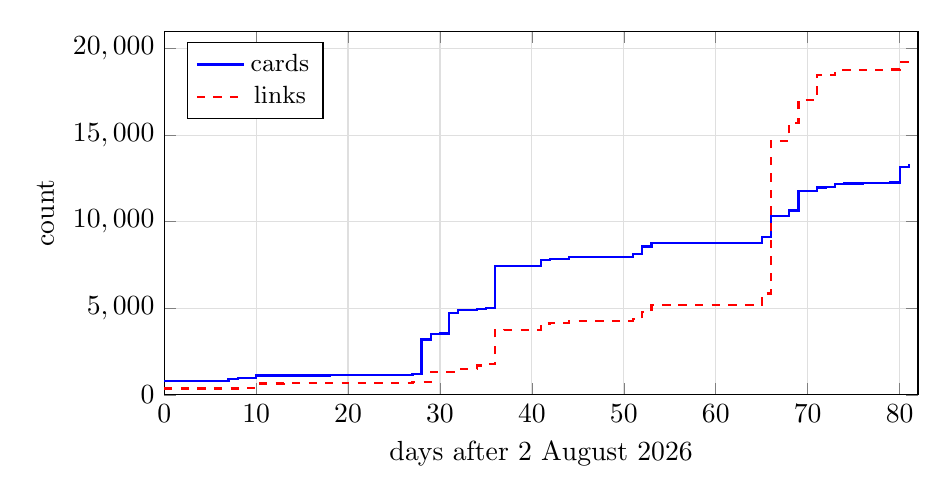
\begin{tikzpicture}
\begin{axis}[
  width=0.92\textwidth, height=6.2cm,
  xlabel={days after 2 August 2026}, ylabel={count},
  xmin=0, xmax=82, ymin=0, ymax=21000,
  legend pos=north west, legend style={font=\small},
  scaled y ticks=false, yticklabel style={/pgf/number format/fixed,/pgf/number format/1000 sep={,}},
  grid=major, grid style={gray!25}]
\addplot[thick, blue, const plot] coordinates {
(0,800)(7,924)(8,958)(10,1114)(13,1121)(18,1131)(20,1155)(27,1191)(28,3191)(29,3526)(30,3538)(31,4732)(32,4895)(34,4970)(35,5006)(36,7433)(37,7443)(38,7450)(40,7451)(41,7803)(42,7865)(44,7947)(49,7975)(51,8114)(52,8568)(53,8772)(54,8776)(55,8776)(59,8778)(64,8785)(65,9105)(66,10319)(68,10650)(69,11753)(71,11979)(72,11982)(73,12188)(74,12200)(75,12207)(76,12213)(77,12245)(78,12247)(79,12257)(80,13178)(81,13306)};
\addlegendentry{cards}
\addplot[thick, red, dashed, const plot] coordinates {
(0,372)(7,372)(8,379)(10,654)(13,663)(18,670)(20,703)(27,735)(28,735)(29,1332)(30,1337)(31,1337)(32,1507)(34,1697)(35,1760)(36,3753)(37,3761)(38,3765)(40,3766)(41,4124)(42,4162)(44,4244)(49,4269)(51,4362)(52,4798)(53,5176)(54,5188)(55,5194)(59,5195)(64,5207)(65,5853)(66,14675)(68,15712)(69,17026)(71,18458)(72,18477)(73,18740)(74,18749)(75,18753)(76,18757)(77,18773)(78,18774)(79,18782)(80,19232)(81,19362)};
\addlegendentry{links}
\end{axis}
\end{tikzpicture}
\caption{Cumulative cards and links (retracted links included), 2 August to 22 October 2026 (day $0$ is 2 August). Steps on days $28$, $31$ and $36$ are harvests of the literature; the step in links on day $66$ (7 October) is a linking pass over existing cards.}
\label{fig:growth}
\end{figure}

\subsection{Links across time}
If agents only ever linked a new card to cards written in the same session, the store would be a set of disconnected notebooks. The record says otherwise. For each link we compare the days on which its two endpoints were created. Of the $19{,}362$ links (the $231$ retracted ones included, about one percent), $12{,}267$ ($63\%$) join cards created on different days, and $9{,}164$ ($47\%$) join cards created thirty or more days apart (Table~\ref{tab:lag}). For dependencies the figure is $4{,}038$ of $9{,}129$, but most of these were written in one pass: on 7 October a linking campaign joined existing cards to the lemmas they use and wrote $3{,}469$ of them. The remaining $569$, written on other days, are the ones that record the intended pattern, a result written in October that uses a lemma written in August while the result was being written.

\begin{table}[ht]
\centering\small
\begin{tabular}{lrrrrr}
\toprule
Kind & same day & 1--6 days & 7--29 days & 30+ days & added after both endpoints\\
\midrule
\texttt{depends\_on} & 3{,}786 & 595 & 710 & 4{,}038 & 667\\
\texttt{cites} & -- & -- & -- & 3{,}603 & --\\
\texttt{analogous\_to} & -- & -- & -- & -- & 300 of 604\\
\texttt{fails\_under} & -- & -- & -- & -- & 114 of 160\\
\midrule
all kinds & 7{,}095 & 1{,}623 & 1{,}480 & 9{,}164 & \\
\bottomrule
\end{tabular}
\caption{The gap in days between the creation of a link's two endpoints. The last column counts links created on a day later than both endpoints: a relation noticed after both results were written. Entries marked -- are not broken out.}
\label{tab:lag}
\end{table}

Two caveats apply to this table. Some long-gap links are automatic: a \texttt{supersedes} link joins a revision to an older one by construction, and a \texttt{cites} link from a new result to an old source says only that the source was in the store; the \texttt{semantic\_association} links are written by a vocabulary pass. The figures that reflect agents working across time are the dependencies with long gaps, the analogies added after both endpoints ($300$ of $604$), and the pitfalls added after both endpoints ($114$ of $160$): in each case an agent noticed a relation between results it had not written.

The table is evidence that work accumulated; it is not a controlled measurement that accumulation helped. A controlled test of a fleet with a shared memory against the same fleet without one, on problems neither has seen, is the subject of Section~\ref{sec:campaign}. The one such comparison we have, on thirteen new open problems, did not favour the brain (Section~\ref{sec:tests}), and we discuss why.

\subsection{What the agents did with it}
The clearest examples are in Section~\ref{sec:math}. On the Fourier entropy-influence conjecture the agents' results on particular classes (the classes on which the inequality was proved with explicit constants, and the routes that failed) were written as cards, linked to the definitions and to each other, and read by later fleets; the reduction proved in Section~\ref{sec:math} was found by a fleet that started from those cards, and its first numerical evidence came from routes recorded as refuted. A card recording a refuted route is cheap to write and saves every later agent the cost of refuting it again; on that campaign the store holds the refutation of a selection lemma at one parameter value and its survival, still open, at another.

\section{What the brain does for an agent: the tests}\label{sec:tests}

\subsection{Protocol}
Every test below compares arms that differ only in access to the brain, with one exception: the layered solving test of Section~\ref{subsec:solve61}, whose fifth layer adds a clock and a hint along with the held notes. The arms use the same model, the same reasoning setting, the same budget of time and tokens, the same tools apart from the brain's, and the same items, and each item is worked by a fresh session so that no arm learns from another. An item is scored correct or incorrect against a private key by a grader that does not see which arm produced the answer. For two arms $A$ and $B$ on the same items, let $n_{AB}$ be the number of items $A$ answered and $B$ did not, and $n_{BA}$ the reverse. The exact two-sided McNemar $p$-value is
\[
p=\min\Bigl(1,\ 2\sum_{j=0}^{\min(n_{AB},n_{BA})}\binom{n_{AB}+n_{BA}}{j}2^{-(n_{AB}+n_{BA})}\Bigr).
\]
We report $n_{AB}$ to $n_{BA}$ beside every $p$. The values quoted were recomputed from the counts by a script included with the paper.

Before reporting a null result we compute the test's room to fail: how many items the better arm could have lost, and whether the instrument could have seen the effect in question. A test in which one arm is already perfect cannot show that arm improving, and its $p$-value says nothing about the brain.

\subsubsection*{Contamination}
The answer to a recall question is, by construction, a card in the store, so the store must not contain the question, its key or an earlier answer to it. Every evaluation passes a retrieval guard that removes, before scoring, every record outside the allowed splits, every answer key, solution, fault annotation and prior evaluation output, the active item and its paired variants, and any record sharing a prohibited source digest. Test sessions are not logged into the link strengths (Section~\ref{sec:strength}). The question banks themselves are kept off the store and out of every repository, so that the same tests can be run on later versions without the answers having been seen. One contamination we cannot rule out is the model's own training data: the arm without the brain may know a published result from pre-training. For published material this is an uncertainty whose direction depends on the outcome measured; for the agents' own results, which were never published before the tests, it does not arise. A second limitation is adaptive: the banks were also used to decide whether packets and ranking changes land, so a result on a bank that informed such a decision is weaker than one on a holdout that no decision touched. The ranking test below was scored on questions held out from its own tuning, but the other banks were reused, and the main comparisons would be stronger on a final holdout that no decision has touched.

\subsection{Three arms on a thousand items}\label{subsec:threearm}
The largest test compares three arms and nothing else. In the first the agent has the brain: the recall tool, served without a shell, and the two prompt hooks of Section~\ref{sec:hook}, and no file tools. In the second it has no brain, no hooks and no recall tool, but it can read, list and search the research repositories, which include the exported store, the campaign records and the open-problem files; the brain's own folders, its transcripts, the keys and every test folder are denied to it. In the third it has the model alone, with no tools. Every arm sees the same system text, the same instructions on how to answer and the same item, one item a session. Claude Sonnet agents (high reasoning) had $600$ seconds an item and Codex agents (gpt-6.1-sol, high reasoning) $900$ seconds. No Claude arm had a shell. For Codex the brain arm had the recall tool and the hook notes and no shell, the documents arm a read-only shell over the same repositories, and the third arm nothing. The runs took place on 23 and 24 October 2026. The Claude run splits the bank into three shards run side by side, and the Codex run takes items the Claude run has already finished; the figures below cover the items that had been run in all three arms by the evening of 24 October, $755$ of the $1{,}000$ for Claude and $182$ for Codex.

The bank was built on 12 September 2026 and has $1{,}000$ items. $923$ are lookups over the store's records: questions on the open-problem ledger (the sum or the difference of the pages on which listed problems are posed in their sources, which of four is posed latest, which source is the odd one out) and on the self-avoiding-walk counts held in the store, each combining two to four records. The other $77$ are proof audits, in which the agent decides whether a numbered proof is correct as written and, if not, names its first invalid step. The lookups test what the memory is for; the audits are a mathematics control, since their answers are not stored anywhere. A timeout or an error without an answer counts as wrong. A session that never reached the model (a refused account or a session limit, recognised by an empty event stream) is dropped and rerun, not graded.

\begin{table}[ht]
\centering\small
\begin{tabular}{llccc}
\toprule
 & & Brain & Documents & No tools\\
\midrule
Claude, $755$ items run in all arms & correct & $94.3\%$ & $78.1\%$ & $21.7\%$\\
 & sessions timed out & $4.8\%$ & $21.2\%$ & $35.8\%$\\
 & mean seconds an item & $136$ & $241$ & $249$\\
Claude, $593$ items both brain and documents & correct & $99.2\%$ & $99.3\%$ & \\
\quad answered in time & & & & \\
Claude, $480$ items all arms answered in time & correct & $99.2\%$ & $99.4\%$ & $34.0\%$\\
\quad of which proof audits, $68$ & correct & $98.5\%$ & $97.1\%$ & $98.5\%$\\
Codex, $182$ items run in all arms & correct & $93.4\%$ & $97.3\%$ & $31.9\%$\\
\quad of which proof audits, $50$ & correct & $98.0\%$ & $94.0\%$ & $92.0\%$\\
\bottomrule
\end{tabular}
\caption{The three-arm test, Claude Sonnet and Codex gpt-6.1-sol, 24 October 2026. ``Documents'' is the arm with the repositories and no brain.}
\label{tab:threearm}
\end{table}

For Claude the brain beat the documents $134$ to $12$ on the items where they disagreed ($p=3.0\cdot10^{-27}$) and the bare model $549$ to $1$; the documents beat the bare model $427$ to $1$. The first of these numbers needs reading with the rest of the table. On the $593$ items that the brain arm and the documents arm both answered within the time, they are tied, $99.2\%$ against $99.3\%$, $2$ to $3$. The brain's lead over the documents is therefore almost entirely time: an agent searching the files finds the same records, but it needs more searches to find them, and on about a fifth of the items it is still searching when the clock runs out. The gap is largest on the walk lookups that need three or four records, where the documents arm answered $31$ to $51\%$ of the items in a family and the brain arm $76$ to $95\%$. All but one of the bare model's timed-out sessions fall on these walk lookups, where it tries to enumerate the walks by hand.

The Codex agents had half again as much time and seldom ran out of it. There the documents arm scored $97.3\%$ against $93.4\%$ for the brain ($3$ to $10$, $p=0.09$; on the lookups alone $1$ to $10$, $p=0.012$, which does not survive the correction of Appendix~\ref{app:stats}). On the first $100$ Codex items every one of the brain arm's losses was an abstention, never a wrong value. In two the agent never called the recall tool. In three its searches missed records that the documents arm found by reading the files; in one of these the record held a string of punctuation and digits, which the recall tool's lexical match handles poorly and a text search finds at once. Neither aid moved the proof audits, which every arm, the bare model included, answered at about the same rate: the store adds nothing to a proof that the model can check by itself.

\subsubsection*{What it cost}
The $923$ lookups were generated by scripts from the store's records, and every key was derived twice, from separate reads, with no disagreement. The $77$ proof audits were written by Claude Opus~5 agents on 12 September 2026 and each key was confirmed by a separate verifier; by the workflow's own record that took $2.3$ million tokens and $32$ minutes. The record keeps the total but not its split between input and output, so the price can only be bounded: at list price, \$5 a million input tokens and \$25 a million output tokens, it lies between \$12 and \$58, and cached input would bring it lower. Table~\ref{tab:threearm-cost} gives the cost of every session of the three-arm runs, timeouts and reruns included. The prices are those the Claude command-line client reports at list price; the runs used subscription accounts, and the Codex client reports no price. A session stopped at its time limit records neither tokens nor a price, so the token and price columns leave out the timed-out sessions.

\begin{table}[ht]
\centering\small
\begin{tabular}{llrrrrr}
\toprule
 & Arm & Sessions & Hours & \multicolumn{2}{c}{Tokens a session} & Price a\\
\cmidrule(lr){5-6}
 & & & & in & out & session\\
\midrule
Claude & brain & $808$ & $30.6$ & $20{,}000$ & $1{,}500$ & \$0.053\\
 & documents & $808$ & $53.2$ & $80{,}000$ & $4{,}000$ & \$0.092\\
 & no tools & $807$ & $54.8$ & $2{,}000$ & $300$ & \$0.010\\
Codex & brain & $227$ & $27.6$ & $45{,}000$ & $400$ & ---\\
 & documents & $231$ & $17.0$ & $57{,}000$ & $600$ & ---\\
 & no tools & $232$ & $14.8$ & $7{,}000$ & $3{,}100$ & ---\\
\bottomrule
\end{tabular}
\caption{Cost of the three-arm runs to 24 October 2026: $3{,}113$ sessions, $198$ session-hours, $107$ million input tokens, $5.7$ million output tokens, and \$125.69 at list price for the Claude sessions.}
\label{tab:threearm-cost}
\end{table}

With Claude the brain arm read a quarter of the documents arm's input, wrote two fifths of its output and used $58\%$ of its session-hours. Counting only the sessions that recorded a price, it cost $58\%$ as much a session; the documents arm's timed-out sessions, four times as many as the brain arm's, are left out of that figure, so the true ratio is probably lower. With Codex the order of the hours is reversed: on the graded sessions the brain arm took $244$ seconds an item against $215$, and its total includes sessions rerun after the connection to the recall server dropped.


\subsection{Recall of results held in the store}
One hundred questions each ask for a fact held in exactly one card. Sixty were reworded so that they share no content word with their card; forty are plain. Codex agents (gpt-6.1-sol, high reasoning) took one question per session. Table~\ref{tab:recall100} gives the five arms.

\begin{table}[ht]
\centering\small
\begin{tabular}{lc}
\toprule
Arm & Correct of 100\\
\midrule
no tools & 0\\
the hook's served notes, no tools & 7\\
text search over a copy of the store's files & 75\\
recall tool (whole cards, identifiers, linked identifiers) & 83\\
hook, recall tool and link walk (the full stack) & 82\\
\bottomrule
\end{tabular}
\caption{Recall of results held in the store, 11 October 2026.}
\label{tab:recall100}
\end{table}

The full stack against the recall tool alone went $2$ to $3$ ($p=1$). This is an estimate of a difference near zero, not a demonstration of equal accuracy: $17$ questions were wrong under the recall tool alone, so there was room for a gain, but a test of this size detects only a large one (Appendix~\ref{app:stats}: at $100$ items and a disagreement rate of $0.2$, power $0.8$ needs a net gain of about $13$). Against text search the full stack went $10$ to $3$ ($p=0.092$). With no tools the agents answered nothing: these are facts that exist only in the store.

The format of the printout decided much of the score. The same retrieval printing titles and $700$-character snippets without identifiers scored $34$; printing identifiers, whole cards and linked identifiers scored $83$.

Cost was measured from the session logs (Table~\ref{tab:recall-cost}). About $98\%$ of all input tokens were cached re-reads of the session, so the saving in uncached input is a factor of $1.8$, not $7.6$. On the first $20$ questions, with the same search tool in both arms, both scored $18$ of $20$; with the walk the sessions read $3.1$ million tokens and made $40$ searches, without it $16.9$ million tokens and $55$ searches. Unlike the rest of the test, these twenty questions were worked in two long sessions an arm rather than one question a session, so the size of that saving is uncertain.

\begin{table}[ht]
\centering\small
\begin{tabular}{lcc}
\toprule
 & Recall tool alone & Hook, recall and walk\\
\midrule
Input tokens, all questions & 186 million & 24.6 million\\
Uncached input tokens per question & 24 thousand & 13 thousand\\
Output tokens per question & 1.9 thousand & 0.4 thousand\\
Session-minutes, all questions & 666 & 78\\
\bottomrule
\end{tabular}
\caption{Cost of the two strongest arms of Table~\ref{tab:recall100}.}
\label{tab:recall-cost}
\end{table}

\subsection{Several wordings}
On a further $100$ held-out questions, the recall tool given two or three wordings of each question in one call answered $86$; given one wording a call (the agent free to call again) it answered $76$. Merged wordings were also the cheapest of the strong strategies, because each call is a turn that re-reads the whole session.

\subsection{Recall that the agent cannot do without the store}
On $13$ September agents answered $1{,}000$ items, each of which requires a fact that is a card in the store. Without the brain they answered $538$; with it, all $1{,}000$. The brain helped on $462$ items, and no harm was observed ($p=1.7\cdot10^{-139}$). The design did not exclude harm; the arm with the brain happened to be perfect, so what the test shows is the size of the gap the store closes on material of its own. It says nothing about reasoning items, which the solving tests below address.

\subsection{Ranking on held-out questions}
This test measures the retrieval engine without an agent: how often the answer card is among the first eight results, on questions that played no part in tuning. On 12 October the ranking was changed from the base profile to the recall profile of Section~\ref{sec:retrieval} after tuning on a development set.

\begin{table}[ht]
\centering\small
\begin{tabular}{lccc}
\toprule
 & Before & After & Gained to lost ($p$)\\
\midrule
584 held-out questions & 298 & 317 & 27 to 8 ($0.0019$)\\
six further sets, 1{,}070 questions & 891 & 1{,}018 & 143 to 16 ($1.1\cdot10^{-26}$)\\
\bottomrule
\end{tabular}
\caption{Answer card in the first eight results, before and after the ranking change of 12 October.}
\label{tab:ranking}
\end{table}

The six further sets moved unevenly: three gained $32$, $44$ and $66$; two that were already near the ceiling with word search alone lost $9$ and $7$; one gained $1$. The ranking was tuned on questions written by Codex agents, and its largest held-out gain is on a set written by Claude agents, which argues against overfitting to one author's phrasing. The gain comes from the ranking, BM25 with $b=0.4$ and titles counted twice; the meaning channel adds about nothing on these sets. On the development check the first-place hits rose from $37$ to $54$ of $142$ and the mean reciprocal rank from $0.331$ to $0.442$.

A proposed embedding of whole cards, built later, put the answer in the first eight for $52$ of $80$ questions against $27$ for the live channel. It has not been switched on, because it has not yet passed the held-out recall gate on the full sets.

\subsection{Files in GitHub repositories}
Questions were drawn from little-known files in GitHub repositories that the store indexes, and Codex agents (gpt-6.1-sol, medium reasoning) answered them with git, with and without the brain. A crash cut the run short. With git and the brain the agents answered $83$ of $90$ correctly; with git alone, $76$ of $90$. Both arms completed the same $80$ questions before the crash, and on those the scores were $73$ and $68$ ($9$ to $4$, $p=0.27$). The brain arm read $14\%$ more tokens per question. When the files are at hand, the brain adds little.

\subsection{Solving and auditing}\label{subsec:solve61}
Sixty-one items, from four pooled runs on 5 and 6 October, asked Claude Sonnet agents to solve a problem or to find the fault in a purported solution, with Python, Lean and file tools and up to $600$ seconds an item. The arms add one layer at a time: tools only; documents; ranked recall; the hook and the recall tool; held notes, a six-minute clock and a hint; and the statement of any named result the item refers to. The full package has every layer.

\begin{table}[ht]
\centering\small
\begin{tabular}{lcccc}
\toprule
Comparison & Items & Scores & Disagreements & $p$\\
\midrule
full package against tools only & 61 & 52 and 41 & 15 to 4 & 0.019\\
the same, without 7 items whose keys proved ambiguous & 54 & 48 and 39 & 12 to 3 & 0.035\\
items that name a known result & 26 & 22 and 13 & 10 to 1 & 0.012\\
items that name none & 35 & 30 and 28 & 5 to 3 & 0.73\\
full package against documents and recall & 61 & 52 and 46 & 10 to 4 & 0.18\\
\bottomrule
\end{tabular}
\caption{Solving and auditing, 5--6 October 2026.}
\label{tab:solve61}
\end{table}

The gain over tools alone is significant at $p=0.019$ as a single comparison but does not survive a Holm correction over all the paired comparisons of this paper (Appendix~\ref{app:stats}), and the full package changes more than the memory: its fifth layer adds a clock and a hint. Within it, the gain lies in the items that name a known result: an agent that is told, correctly, what a cited theorem says catches a misuse of it that an agent working from its own memory misses. Against agents that already have the documents and a recall tool, the further gain is not significant. Served notes cut both ways here. They helped on faults that drop a hypothesis, and they hurt on faults of citation, scope and sharpness, where a note about the cited result made a wrong use of it look legitimate; that observation is the reason for the trust line of Section~\ref{sec:hook}.

\subsection{What did not help}

\subsubsection*{Spreading activation}
Agents told why each card came up scored $79$ with spreading and $80$ without, while reading $46\%$ more input tokens. Without agents, on the $584$ questions, spreading moved first-eight hits from $298$ to $307$ but found no card the word search had missed: it re-ranks and nothing more. It is off by default.

\subsubsection*{A pointer to the next card}
A line printed under the cards, naming the card most often reached next from them, was tested on 15 October. Without agents it changed no ranking on the $584$ held-out questions, lost no answer, and on $6$ of them named an answer card that the printout showed nowhere else. Codex agents (gpt-6.1-sol, medium reasoning, ten questions a session) then answered $60$ further held-out questions, $30$ hard and $30$ plain, under three printouts of the recall tool: the printout of before 12 October, the current one, and the current one with the line. They answered $48$, $48$ and $45$ correctly ($28$, $28$ and $26$ of the hard questions). Against the current printout the line went $0$ to $3$ ($p=0.25$), and one of the three losses gives the right number in another notation; the agents opened $7$ of the $220$ cards the line named. The current printout against the earlier one went $2$ to $2$ ($p=1$) and read $16\%$ less uncached input a question ($10.1$ against $12.0$ thousand tokens). The $18$ sessions read $52$ million input tokens, $96\%$ of them cached re-reads, and wrote $75$ thousand. The line was not adopted. All three arms ran with the agents' ordinary start-up hooks, so their level is not comparable with Table~\ref{tab:recall100}, and at $60$ questions the test sees only a large effect.

\subsubsection*{New open problems}
Fourteen Codex agents worked $13$ open problems on which the store held only a first attempt, written in September. Each attempt was graded blind at up to $3$ points. The arm with the brain scored $24$ of $39$ and the arm without it $26$; a referee comparing each pair preferred the attempt without the brain $8$ times and the one with it $3$ times, with $2$ even ($p=0.23$). The store held almost nothing on these problems beyond a first attempt, so this test measures what the brain adds when it has little to recall, and the answer is nothing measurable. It does not measure the case for which the brain was built, a problem on which earlier agents have left many results.

\subsubsection*{An early version against plain documents}
On a hard set of $300$ items with no tools, version $1$ of the system (hook notes, the recall tool, Lean and an audit step) scored $238$, and agents given the documents directly scored $264$ ($14$ to $40$, $p=0.0005$). Most of the loss was in one group of $70$ items, $22$ against $55$, where the version-$1$ hook served notes that pulled agents off the documents. The later version, which routes to deliberate recall first, adds a clock and silences the hook on weak matches, was built in response to this result. On 4 October that version (lookup in the store first, Lean at most once with a limit of $90$ seconds, a $360$-second clock), run by Claude Sonnet agents on $110$ problems answerable from the store, scored $102$ against $104$ for agents given the documents and a recall tool ($6$ to $8$, $p=0.79$). The items and the baseline differ from those of the $300$-item run, so the two results do not form a before-and-after pair; the second shows neither a loss nor a gain against documents with recall.

\subsection{Deliberate recall over time}
The deliberate recall path was itself improved by the tests. On a fixed set of $64$ questions on the agents' own past work, the answer was first for $24$ questions in September and for $46$ after the changes described in Sections~\ref{sec:retrieval}--\ref{sec:hook}. On a larger held-out set the recall tool answered $317$ of $584$, against $298$ before the ranking change.

\begin{figure}[ht]
\centering
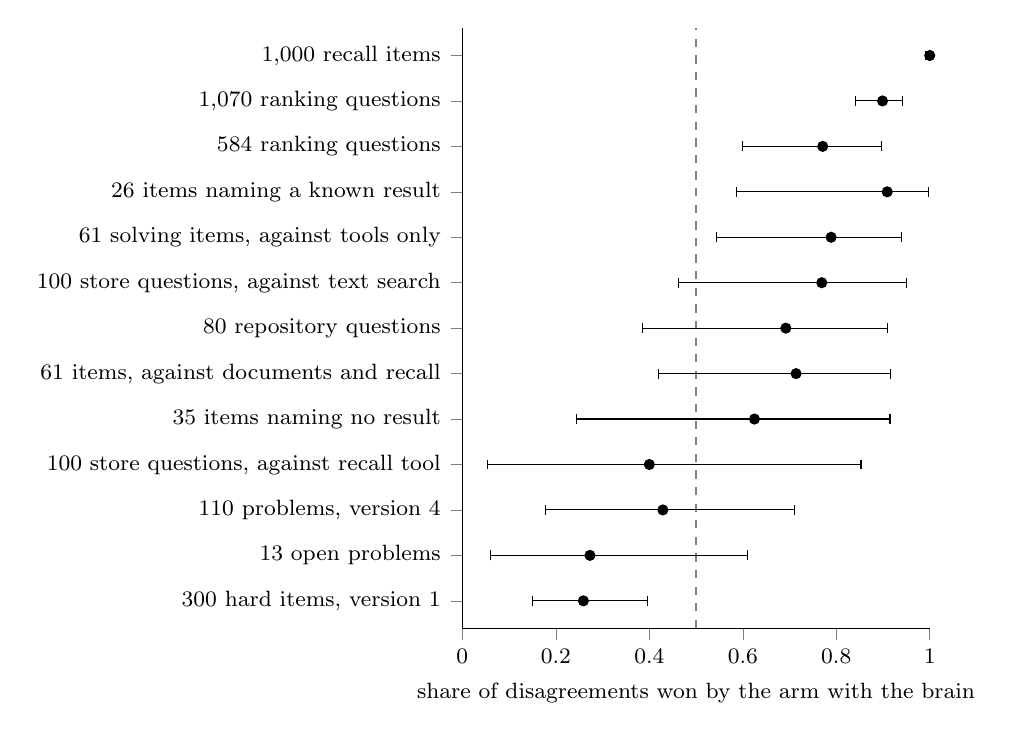
\begin{tikzpicture}
\begin{axis}[
  width=0.62\textwidth, height=9.2cm,
  xmin=0, xmax=1, ymin=0.4, ymax=13.6,
  xlabel={share of disagreements won by the arm with the brain},
  ytick={1,...,13},
  yticklabels={
    {300 hard items, version 1},
    {13 open problems},
    {110 problems, version 4},
    {100 store questions, against recall tool},
    {35 items naming no result},
    {61 items, against documents and recall},
    {80 repository questions},
    {100 store questions, against text search},
    {61 solving items, against tools only},
    {26 items naming a known result},
    {584 ranking questions},
    {1{,}070 ranking questions},
    {1{,}000 recall items}},
  yticklabel style={font=\footnotesize},
  xticklabel style={font=\footnotesize},
  xlabel style={font=\footnotesize},
  tick align=outside, axis x line*=bottom, axis y line*=left,
]
\addplot[gray, dashed] coordinates {(0.5,0.4) (0.5,13.6)};
\addplot[only marks, mark=*, mark size=1.8pt, black,
  error bars/.cd, x dir=both, x explicit]
  table[x=s, y=y, x error minus=m, x error plus=p] {
  y  s      m      p
  1  0.259  0.109  0.138
  2  0.273  0.213  0.337
  3  0.429  0.252  0.282
  4  0.400  0.347  0.453
  5  0.625  0.380  0.290
  6  0.714  0.295  0.202
  7  0.692  0.306  0.217
  8  0.769  0.307  0.181
  9  0.789  0.245  0.150
  10 0.909  0.322  0.089
  11 0.771  0.172  0.125
  12 0.899  0.057  0.042
  13 1.000  0.008  0.000
  };
\end{axis}
\end{tikzpicture}
\caption{The comparisons of the brain against a baseline on one scale: the share of the disagreeing items won by the arm with the brain, with an exact $95\%$ Clopper--Pearson interval. The dashed line is no effect. The four lowest rows are tests on which the brain did not help; the rows for versions~1 and~4 concern earlier versions on item sets and baselines of their own, and the open-problems row is a referee's pairwise preference. Intervals that cross the line are inconclusive, not evidence of equal accuracy.}
\label{fig:effects}
\end{figure}


\subsection{What the tests say}
Figure~\ref{fig:effects} puts the comparisons of the brain against a baseline on one scale, the losses and the inconclusive results included. The pattern across tests is consistent. The brain helps when the answer is something the agent cannot know: a result in the store and nowhere else ($538$ to $1{,}000$), or, less firmly, a cited theorem whose exact statement decides whether a proof is right ($13$ to $22$, a subset result that does not survive the correction for several comparisons). It saves cost when the agent can move along links instead of searching again (uncached input fell by a factor of $1.8$, with $82$ and $83$ correct). When the agent already has the documents and enough time, it finds the same records, and the brain adds speed and lower cost rather than accuracy: the three-arm test tied on the items both arms finished, and under a ten-minute limit that speed separated $94\%$ from $78\%$. It adds nothing measurable on a new problem about which the store knows nothing. The size of the effect is set by what is in the store, which is why the store's growth and the write-back path matter as much as the retrieval.

\subsection{The test bank}
The tests draw on a private bank of items written for the purpose. On 22 October $6{,}778$ items had been written and $256$ admitted. An item is admitted only after two independent audits agree that its key is correct and unambiguous, that it is answerable from the store for the recall strata, and that it is not answerable from the public files of the release (seventeen items answerable from the release files were retired). Admission is the bottleneck, not writing: most items fail on key repair, not on the audits. The bank, its keys and the per-item records are not published; anchors committing to the content of the blinded experiments are public, so that a later reader can check that the reported items were fixed before the runs.

\section{The ensemble and long-horizon campaign}\label{sec:campaign}

The tests of Section~\ref{sec:tests} ask what the brain does for one agent answering one question. The case for which the brain was built is different: many agents, over many days, on problems where each agent's work is supposed to become the next agent's starting point. A campaign to measure that case directly began on 22 October 2026 and is not complete. We give its design, because the design is what makes such a comparison informative, and because it can be repeated by anyone with the released store.

\subsection{Design}
Each arm is a fleet: a fixed number of agents of one model, working in rounds on a fixed set of problems for a fixed number of days, with the same work orders and the same compute and token budgets. The arms differ in what persists between rounds.
\begin{enumerate}[label=(\alph*)]
\item \emph{No memory.} Each round starts from the problem statements only.
\item \emph{Shared notes.} Each round reads a shared folder of the previous rounds' reports, with text search over it.
\item \emph{The brain.} Each round reads the store and lands its results through the write-back path of Section~\ref{sec:writeback}; the next round recalls them.
\end{enumerate}
Arm (b) is the control that matters. A brain that beats arm (a) but not arm (b) adds nothing over writing things down.

\subsection{What is measured}
For each problem and each round, a grader that does not know the arm scores the best current result on a fixed rubric (proved, verified by computer, refuted, partial, nothing). The primary measures are the score at the last round and the area under the score curve over rounds, compared between arms by paired tests over problems. Secondary measures are the number of times an arm re-derives a result an earlier round had already established, the number of times it repeats a route an earlier round had recorded as refuted, and the cost per point of score in input tokens, uncached input tokens and session time. A cost ledger records every session of every arm.

\subsection{Controls}
Problems are drawn from rows of the problem list on which the store holds little, so that the brain arm has no head start from material written before the campaign; a second stratum uses rows on which the store holds a great deal, to measure the head start itself. The question banks of Section~\ref{sec:tests} are not used. The campaign's own records enter the store only after the campaign ends.

\section{The mathematics}\label{sec:math}

The store was built to be used for research, and the agents that built it were doing research while they built it. This section reports what came of that work. We separate four kinds of statement: \emph{proved} (a complete proof is given here or in a cited paper of this project), \emph{verified by computer} (a certificate checked by rigorous arithmetic or a proof assistant), \emph{evidence} (finite computation in floating point or a search that found no counterexample), and \emph{open}. None of the results below has yet been refereed by a journal, and several have been checked only by agents; we say which.

We do not claim that the brain produced these results. Some were obtained before the store held more than a few hundred cards, and none comes from a controlled comparison with agents working without it. What the store did, and what can be checked in its records, is hold the definitions, the failed routes and the partial results of each campaign so that later agents started from them.

\subsection{The problem list}
On 10 October the work was focused on a list of open problems in probability theory, chosen to be important, publishable and plausibly within reach, and later extended by a second list in the theory of deep learning. On 22 October the list had $422$ rows: $222$ in probability (T001--T222) and $200$ in deep learning (T223--T422). Before an agent starts a row it searches the literature and public code for an existing solution; $22$ rows have been retired because others had solved them, $16$ of them in 2026 and $3$ of those with credit to AI systems. A row counts as solved only when its central obstruction is removed. A new constant, a special case or a numerical improvement is recorded as progress and leaves the row open. A claimed answer is a candidate until two independent audits pass.

By that rule one row has been solved, T069, the capacity of the Ising perceptron (Section~\ref{subsec:perceptron}). Table~\ref{tab:rows} lists the other rows that moved in the last days before this paper was written.

\begin{table}[ht]
\centering\small
\begin{tabular}{lp{9.2cm}l}
\toprule
Row & Result & Status\\
\midrule
T228 & exact power-law tail of scalar leaky-ReLU stochastic gradient descent with fresh Gaussian samples (one target of the row) & proved, reviewed\\
T336 & normalized ReLU attention with at most $5$ heads, width $7p+4$ and depth of order $\sqrt\kappa\,\log(2/\delta)/2$ computes the Gaussian-process noisy predictive mean and variance in context, by a Chebyshev iteration (one target of the row) & proved, reviewed\\
T353 & a counterexample to Conjecture 3.2 of Chua et al.\ on DP-SGD with shuffled batches; the row stays open & posted\\
T354 & a rate theorem for nonconvex Adam with random reshuffling (frozen drift plus remainder) & provisional\\
T357 & a closed first-order form for the regularization gap of random-features ridge regression & provisional\\
T366 & on one family of clusters, the quantity of Condition (B) is bounded near $(3+\sqrt{21})/6\approx1.2638$ & partial\\
T248, T421 & an edge case placed on three representations; the critical Adam tail is invisible in floating point and appears in multiple precision & provisional\\
\bottomrule
\end{tabular}
\caption{Rows of the problem list that moved between 20 and 22 October 2026. Only T069 is solved.}
\label{tab:rows}
\end{table}

Outside the list, the agents posted an answer to Question 16.7 of Lyons and Peres: the two natural measures $\nu_2$ and $\nu_3$ on the Cantor set are mutually singular. The proof has not yet been checked independently.

\subsection{The Ising perceptron at zero margin}\label{subsec:perceptron}
Let $g_1,g_2,\dots$ be independent standard Gaussian vectors in $\R^N$ and let $M_N$ be the largest $M$ for which some $\sigma\in\{-1,1\}^N$ satisfies $\langle g_a,\sigma\rangle\ge0$ for all $a\le M$. Krauth and M\'ezard \cite{KrauthMezard1989} predicted that $M_N/N$ converges to an explicit constant $\alpha_*\approx0.833$. Ding and Sun \cite{DingSun2019} proved the lower bound subject to a numerical condition on a two-parameter function, and Huang \cite{Huang2024} proved the upper bound subject to a second numerical condition on a moment functional. Both conditions had been checked numerically in floating point and not proved.

The agents verified both conditions in ball arithmetic (Arb, through \texttt{python-flint}). The Ding--Sun condition was certified on a grid of $247$ cells with positive and negative derivative ranges, strict curvature at the left end and an analytic one-sided derivative condition at the right end. The Huang condition was certified after compactifying the moment body, by two bulk sweeps, a constructive neighbourhood of the fixed point and a cover of the remaining region by rays on which the functional is concave. Every accepted inequality is recomputed in ball arithmetic from the stored certificate; a helper that proposes rational duals, tilts and boxes in floating point is never trusted. Together with the two conditional theorems this gives
\[
\frac{M_N}{N}\to\alpha_*\quad\text{in probability},\qquad \alpha_*\in[0.833078599,\ 0.833078600].
\]
The certificates pass their verifiers and a separate audit by a second AI system; the proof has not yet been reproduced independently or peer reviewed (arXiv:2607.11010; repository \texttt{ising-perceptron-capacity}). Most of this work was done in July 2026, before the store held its present content, and we do not count it as evidence for the brain. A companion paper treats nonzero margin.

\subsection{The Fourier entropy-influence conjecture}\label{subsec:fei}
For $f:\{-1,1\}^n\to\{-1,1\}$ write $\hat f(S)$ for its Fourier coefficients, $p(S)=\hat f(S)^2$ (a probability law on subsets of $[n]$, by Parseval), $H(f)=\sum_S p(S)\log_2(1/p(S))$ for the Fourier entropy, $\Inf_i(f)=\sum_{S\ni i}p(S)$ for the influences, $I(f)=\sum_i\Inf_i(f)$ for the total influence, and $\Var f=1-p(\emptyset)$. Friedgut and Kalai \cite{FriedgutKalai1996} conjectured that $H(f)\le C\,I(f)$ for an absolute constant $C$. The conjecture is open; the best lower bound on $C$ is $6.4548$, from a construction of Hod \cite{Hod2017}, and it has been proved on many classes, among them symmetric functions and read-once decision trees \cite{OWZ2011} and read-once formulas \cite{OT2013}.

From 21 September to 22 October the conjecture was the target of the largest campaign the store recorded: scheduled agents running every hour, one hundred Codex agents in twenty streams on 11 and 12 October, and a group of routes each worked by one strong agent with an independent referee. Its record in the store is a set of cards for the definitions, the equivalent forms, the classes on which the inequality is known, about thirty routes that failed with the example that kills each, and the results below.

\subsubsection*{The reduction}
For a set $S$ put $\pi(S)=\sum_{T\supseteq S}p(T)$, the mass above $S$, and define
\[
U(f)=\sum_{S:\,p(S)>0}p(S)\log_2\frac{\pi(S)}{p(S)}.
\]
Since $p(S)\le\pi(S)\le1$, we have $0\le U(f)\le H(f)$. $U$ is additive over functions of disjoint sets of variables, vanishes when the spectrum is an antichain (for instance when $f$ is homogeneous of some degree), and compares each Fourier weight with the weight sitting above it in the subset order. The quantity $\pi(S)$ is the generalized influence of \cite{KKLMS2020}: if $d_Sf(z)$ is the top coefficient of the restriction of $f$ to the variables in $S$ with the others fixed to $z$, then $\pi(S)=\EE_z[(d_Sf)^2]$ and $\hat f(S)=\EE_z[d_Sf]$.

\begin{lemma}\label{lem:Gkey}
For every Boolean $f$ and every nonempty $S$, $|\hat f(S)|\le 2^{|S|-1}\pi(S)$. Equivalently $p(S)\le4^{|S|-1}\pi(S)^2$. \proofbutton{lem:Gkey}
\end{lemma}

For $|S|=1$ this is the familiar inequality $|\hat f(\{i\})|\le\Inf_i(f)$. The lemma holds with equality for every set in the spectrum of a point defect, and an exact integer check over all $984{,}884$ pairs $(f,S)$ with $n\le4$ found $266{,}492$ equalities and no violation. It is the only place where the proof uses that $f$ takes values $\pm1$, through the parity of a sum of $2^{|S|}$ signs.

Theorem~\ref{thm:intro-G} follows from the lemma and the identity $H(f)=\sum_Sp(S)\log_2(1/\pi(S))+U(f)$; the proof is in Appendix~\ref{app:proofs}. It reduces the conjecture to the single statement
\begin{equation}\label{eq:MU}
U(f)\le K\,I(f)\quad\text{for every Boolean }f,
\end{equation}
with $C\le2+2K$; conversely the conjecture with constant $C$ gives \eqref{eq:MU} with $K=C$, and Hod's bound forces $K\ge2.227$. On every function with $n\le4$ the bound of Theorem~\ref{thm:intro-G} holds with minimum slack $0$. More is true: the first inequality of Theorem~\ref{thm:intro-G} is an equality for point defects, for the addressing functions, for the bent function on two variables, and for every read-once formula built from two-input gates of AND type (Proposition~\ref{prop:readonce-eq} in Appendix~\ref{app:fei}). The read-once AND/OR formulas include the lexicographic functions and the near-extremal formulas found by a beam search, whose ratios $H/I$ rise from $3.40$ to $5.91$; on all of them the conjecture is exactly the statement $\sup U/I<\infty$. The statement \eqref{eq:MU} is not contradicted by Slote's counterexample to the quantum analogue of the conjecture \cite{Slote2026}: Slote's operators are homogeneous, and when the order on Pauli strings is taken letter by letter $U$ vanishes on them. Unlike the conjecture itself, \eqref{eq:MU} is therefore not ruled out by this example for proofs that use only hypercontractivity and operator identities.

\subsubsection*{Restriction}
For a coordinate $i$ let $f_{i,\pm}$ be the restrictions $x_i=\pm1$, $\Delta_iU(f)=U(f)-\frac12(U(f_{i,+})+U(f_{i,-}))$, and $G(f)=\sum_i\Delta_iU(f)$. Proposition~\ref{prop:Uloc} in Appendix~\ref{app:fei} proves the exact identity
\[
\Delta_iU=B_i-\Gamma_i+K_i,
\]
where $B_i=H(S_i\mid S\setminus\{i\})$ is the conditional entropy of the indicator of $i$ under $S\sim p$, $\Gamma_i=\sum_{S\ni i}p(S)\log_2\bigl(\pi(S\setminus\{i\})/\pi(S)\bigr)\ge0$, and $K_i\ge0$ is a sum of binary Kullback--Leibler divergences between the asymmetries of a coefficient and of the mass above it under the two restrictions. It is Proposition~\ref{prop:Uloc}, proved in Appendix~\ref{app:fei}, where it is also checked against direct restriction to $50$ digits; no other result of the paper depends on it. Its meaning is the point. The local logarithm that defeats every coordinatewise charge for $H$, visible in selector functions for which $\Delta_iH/\Inf_i$ grows like the number of address bits, cancels between $B_i$ and $\Gamma_i$: on the same functions, at every size computed, $\Delta_iU/\Inf_i$ stays below $4.31$.

Theorem~\ref{thm:intro-GU} turns a bound on $G$ into the conjecture. Its hypothesis with $b=0$ is the statement we call GU:
\begin{conjecture}[GU]\label{conj:GU}
There is $K<\infty$ such that $G(f)\le K\,I(f)$ for every Boolean $f$.
\end{conjecture}
By Theorem~\ref{thm:intro-GU} with $a=K$, $b=0$, GU implies the conjecture with $C\le2+2K$. It is stronger than the conjecture and is not known to follow from it.

\subsubsection*{Evidence}
Table~\ref{tab:GU} collects the largest values of $G/I$ found. The first searches stopped at $3.090$, attained by the majority of three composed with a five-variable function $g_5$ whose Fourier coefficients lie in $\{\pm4,\pm12\}/32$. The referee of the route, using an independent composition engine, went higher: the majority of five composed with $g_5$ gives $3.2157$, and a six-variable inner function found by annealing under the majority of five gives $3.2265$. No family tried grows: iterating the majority of three over $g_5$ settles near $3.11$, and majorities of larger arity fall ($\mathrm{maj}_7$ gives $3.00$, $\mathrm{maj}_9$ gives $2.70$). If $G\le3.2265\,I$ held in general the conjecture would follow with $C\le8.45$, against Hod's lower bound $6.4548$. On the near-extremal read-once family $G/I$ levels off near $2.29$, and $2+2(2.29)=6.58$.

\begin{table}[ht]
\centering\small
\begin{tabular}{lc}
\toprule
Functions searched & largest $G/I$\\
\midrule
all functions with $n\le4$ & 2.75\\
simulated annealing, $n=5,\dots,8$ & 2.8203\\
$\mathrm{maj}_3\circ g_5$ & 3.090\\
$\mathrm{maj}_3\circ\mathrm{maj}_3\circ g_5$, $\mathrm{maj}_5\circ g_5$ & 3.1581, 3.2157\\
$\mathrm{maj}_5\circ h_6$, $h_6$ found by annealing & 3.2265\\
$\mathrm{AND}_2\circ g_5$, $\mathrm{OR}_3\circ g_5$, $\mathrm{AND}_3\circ g_5$, $\mathrm{AND}_4\circ g_5$ & 2.965, 2.959, 2.806, 2.727\\
near-extremal read-once formulas with $H/I$ from $4.40$ to $5.91$ & 1.94 rising to 2.285\\
tribes & $\le2.19$\\
lexicographic functions & $\le2.19$\\
threshold functions & $\le2.21$\\
random functions, $n=12$ & about 1.0\\
majority, addressing, recursive majority & negative\\
\bottomrule
\end{tabular}
\caption{The largest ratio $G/I$ found in each search. All values are computed in floating point.}
\label{tab:GU}
\end{table}

The coordinatewise strengthening, $\Delta_iU\le K\,\Inf_i$ for \emph{every} $i$, is not supported: annealing over selector pairs $f=(y\,?\,g:h)$ reaches $4.78$, $5.11$, $5.48$ and $6.15$ at $n=6,7,8,9$, driven by the Kullback--Leibler term. This growth over four sizes is evidence, not a proof, that no constant bounds each coordinate; a proof of GU should therefore expect to sum over the coordinates or to choose a good one. The weaker hypothesis of Theorem~\ref{thm:intro-GU} with $b>0$ has only partial support. Every function with $n\le4$ satisfies $G\le2.25\,I+0.5\,U$, but the inequality fails for $\mathrm{maj}_3\circ g_5$ ($3.0905>3.008$) and for $\mathrm{maj}_5\circ g_5$; the fit $G\le1.75\,I+U$ survives every case computed, but $b=1$ lies outside the theorem. For comparison, the analogue for $H$ sits exactly at the threshold, $\sum_i\Delta_iH\le H+(2/\ln2)I$, which is why restriction induction on $H$ itself cannot close.

\subsubsection*{Routes that failed}
The store keeps each failed route with the example that kills it, and these cards were read more than any other part of the campaign's record. Among them: random restrictions with entropy accounting, which give only $C=O(\log n)$; the pivotal-set entropy $H(\mathrm{Piv})\le C\,I$, false on point defects; normalized R\'enyi entropies of order below one, false on tensor powers of point defects; level-only bounds obtained by symmetrizing $U$, which are not stable under tensor products; and transport-entropy lower bounds on total correlation, which are quadratic where a logarithm is needed. A further obstruction is logical rather than computational: any argument whose every step remains true for quantum Boolean functions and their Pauli spectra proves a statement that Slote's operators violate, so a proof of the conjecture must use a property special to classical functions, such as the integrality of Walsh coefficients that Lemma~\ref{lem:Gkey} uses.

\subsubsection*{Classes}
The routes produced inequalities with explicit constants on several classes. None proves the conjecture, and some have not yet been compared carefully with the literature.
\begin{enumerate}[label=(\roman*)]
\item On the class in which every conditional row law is a product, $H\le4I$, and the optimal constant is $16/3-\frac32\log_23\approx2.95589$, attained by the conjunction of three variables. The proof has a computer step certified twice by different rigorous algorithms; an agent of the Codex fleet reached the same constant independently.
\item For every weighted threshold function and every product measure $\mu$, $E_\mu\le\Var\cdot\ln(1/\Var)+A_0\,I_\mu$ with $A_0<9.21$ nats, where $E_\mu$ and $I_\mu$ are the spectral entropy and total influence under $\mu$. A level-wise reference conjecture is refuted by a new family, anti-diagonal tribes thresholds. A related paper treats threshold functions and their compositions.
\item For multiplexers there is an exact cost identity, $\mathrm{cost}(F)=H(S\mid T)+I(X;Y)$, with closure constant $4$. A sharp bound for orthogonal leaves is refuted in $60$-digit interval arithmetic; a defect conjecture with constant $\kappa_0=0.756151564$ is open, and searches in double precision or at $30$ digits produce values above $\kappa_0$ that disappear at $60$ digits.
\item $H\le10.38\,I$ on selector trees, $H\le16.99\,I$ on selector trees with regular leaves on fresh blocks, and $H\le26.71\,I$ on term decision lists with a common output mean.
\end{enumerate}

\subsection{Other problems and the papers}
Thirty-one papers came out of the work recorded in the store, each with its own public repository; Appendix~\ref{app:papers} lists them. They range over random allocations and condensation, Galton--Watson trees, mixing and relaxation of Markov chains, free probability, random-cluster measures, percolation, the Ising perceptron, Boolean functions and deep networks, and one is a library of probability proof components in Lean. They differ in how far they have been checked: some have been read line by line by the author, some only by agents, and none has yet been refereed by a journal.

\section{Using the brain}\label{sec:usage}

This section is for a reader who wants to use the store, add to it, or repeat the tests. Appendix~\ref{app:tools} lists every tool with its options.

\subsection{Installing}
The release is a Python package with the store exported as text, one JSONL file per table, so that it can be read, diffed and reviewed without the database. The import command builds the database and reports card and bundle-manifest digest failures:
\begin{verbatim}
pip install -e .
python tools/import_store.py --out local/population/brain.sqlite3
export MATHBRAIN_STORE=local/population/brain.sqlite3 MATHBRAIN_BUILD_SRC=src
\end{verbatim}
The importer reports digest mismatches; its exit status alone is not a certificate that all digests passed. Run the release-integrity checker supplied with this paper for an explicit fail-on-mismatch check. The meaning channel requires the separately configured encoder and vector index; importing the database alone does not build that model. Word-based recall remains available without it.

\subsection{Asking}
A question is asked in words, the way a card would state the answer:
\begin{verbatim}
python agent_tools/math_recall.py \
    "spectral gap of the random transposition walk" \
    --or "relaxation time of random transpositions on S_n"
\end{verbatim}
The tool prints eight whole cards with their identifiers and the identifiers of their links. Three habits account for most of the measured gains.
\begin{enumerate}[label=(\roman*)]
\item \emph{Give two or three wordings in one call}, each after its own \texttt{--or}, and word them the way a card would: the object, the theorem or method by name, the symbol, the author. This raised the score from $76$ to $86$ of $100$.
\item \emph{Walk instead of searching again.} When a printed card is on the right topic but is not the answer, open its neighbours with \texttt{--id} or walk from it with \texttt{math\_walk.py <id> --toward "<what you need>"}. Walking reached the same answers as searching again at about half the uncached tokens.
\item \emph{Stop when a card answers, and reword on a weak match.} A \texttt{WEAK MATCH} line means the words are wrong, not that the store is empty; after three rounds of wordings with nothing, report that the card was not found by this search, which is weaker than saying the store does not hold it.
\end{enumerate}
Leave spreading off. It re-orders what the words found and costs about half again as many tokens.

\subsection{An example}
The following call was made on 23 October 2026 against the store of that day; it returned in $14$ seconds.
\begin{verbatim}
python agent_tools/math_recall.py \
    "Fourier entropy influence conjecture constant" \
    --or "read-once formula entropy influence bound" \
    --or "FEI gate potential inequality"
\end{verbatim}
It printed eight cards. The first is the statement that every read-once formula $f$ over AND, OR and NOT satisfies $H(f)\le 6.4573\,I(f)$, with the identifier \texttt{claim\_415d9ba1b7f745a2a442da84ef6836ef}. Its header says that the second wording ranked it first and the first wording eighth, and lists the words it matched. Among the links printed below the statement: it specializes the open problem on Fourier entropy and total influence, it depends on the cards for influence and Shannon entropy, and an evidence card records the interval-arithmetic certificate behind the constant, cross-checked at $40$ digits. The second card, ranked first by the third wording, is the reformulation of FEI as a single inequality over Boolean gates (Section~\ref{sec:math}), whose evidence card records the sweep in which the two-input AND is the binding gate. The remaining six are the conjecture's definition card, the threshold-function result, the restriction-induction floor of $7.05$, a question card on the biased form, an attempt record, and the Kahn--Kalai--Linial card.

For a reader who wanted the constant and its proof, the first card answers, and the search stops there. One link was not printed; \texttt{--id claim\_415d9ba1} prints the card with all of them.

\subsection{The hook}
The hook is installed in the agent runtime as a command that runs on each prompt. It reads the prompt, runs the base-profile search, and prints at most a few cards with a trust line under each, or nothing. Section~\ref{sec:hook} gives its gates. An agent should treat a served card as a lead to open with \texttt{--id}, not as an answer; the hook is silent on most questions and is not the recall path.

\subsection{Writing back}
A result is added as a packet: a folder with one file per new card (statement, conditions, proof text or certificate, source, kind) and one file of links into the store by identifier. The packet tool validates it, computes its digest, runs the held-out recall gate on a copy of the store, and lands it in one transaction if every check passes. Four rules keep the store useful.
\begin{enumerate}[label=(\alph*)]
\item State hypotheses exactly. A card that drops a hypothesis is worse than no card, because the next agent will use it.
\item Record failures. A refuted route with its counterexample, joined by \texttt{refutes} or \texttt{fails\_under} to what it concerns, is among the most read cards in the store.
\item Link to what the result uses. A card with no links can be found only through its words; a card with \texttt{depends\_on} links appears in the exact closure of everything built on it.
\item Never edit; supersede. A corrected statement is a new revision with a \texttt{supersedes} link to the old one.
\end{enumerate}
A new card enters as \textsf{unverified}. Changing its status requires evidence through the verification router of Section~\ref{sec:writeback}.

\subsection{Repeating the tests}
The tests of Section~\ref{sec:tests} can be repeated as regression tests on a later version of the store, or on a different store. Keeping the question banks private does not make such repetitions fresh held-out evaluations after the answer-bearing material has been released. The harness takes a bank, a list of arms and a model, runs each item in a fresh session per arm, applies the contamination guard, grades blind against the keys, and writes per-arm scores, the discordant counts, the exact McNemar $p$-values and a cost ledger. An arm is a configuration: which tools the agent may call, whether the hook runs, which copy of the store it reads, and the budget. The two arms of a comparison must differ only in the brain.

The banks are kept by the authors and are not in the release. A researcher who wants a test run on a new version may send the version; a researcher who wants to build a bank of their own should follow three rules. Write items whose answers are cards and audit each key twice before admitting it; exclude from any fresh held-out bank items answerable from public files or previously used for tuning; and before reporting a null result, compute whether the test had room to show the effect.

\subsection{Several agents}
For several agents on one problem, the arrangement that worked was a work order that names the target, the cards already known (by identifier), what is ruled out and what counts as progress; a shared folder for reports; and one agent whose job is to turn reports into packets. Agents that write to the store directly in parallel are safe, because a bundle either lands whole or not at all and the landing checks are made inside the transaction, but they duplicate each other's work unless the work order divides it.

\section{Limitations and the public release}\label{sec:limits}

\subsection{What the tests do not show}
The tests measure one agent answering one question. The case the brain was built for, many agents extending one body of work over weeks, is supported by the record of Section~\ref{sec:collective} but has not been measured by a controlled comparison; the one comparison on new problems did not favour the brain, and the store held almost nothing on those problems. Section~\ref{sec:campaign} describes the comparison that will settle this.

Every test used agents of two vendors at particular model versions. Models change every few months, and a stronger model may need the store less for material it can derive and as much for material it cannot know. The measured effects are therefore statements about these agents and this store, and private question banks support controlled regression runs; they do not by themselves prevent future training-data contamination.

The no-brain arm may know published results from its training. For literature cards this makes the measured gains conservative. The store is now public, so its own cards may enter the training data of later models, and a later no-brain arm may then know the agents' own results as well; a test of a later model against this store will understate the brain's effect for a reason that has nothing to do with the brain. Fresh evaluation banks should be drawn from unseen material and checked against the released files and the model's documented training boundary where available.

\subsection{What the store does not guarantee}
Most cards are \textsf{unverified} or \textsf{provisional}. The store records what was claimed, by what route and with what support; it does not certify that the claims are true. The curated secondary cards were written by agents from textbooks and surveys, and a card can misstate a hypothesis of its source; the fidelity of statement to source has been reviewed for many cards but not all. A reader who uses a card in a proof should read its source.

The store is unevenly distributed. It is dense in probability theory, Boolean functions and the theory of deep learning, where the campaigns were, and thin elsewhere; $2{,}878$ cards have no link and can be found only by their words.

The retrieval is a word search with a meaning channel. It does well when the question can be worded the way a card is, and poorly when it cannot: the hook was silent on all $60$ reworded questions of the store test. A whole-card embedding that does better on reworded questions has been built and not yet switched on.

\subsection{Cost}
A search prints about $11{,}000$ characters, and an agent that searches many times pays for every printout again at each later turn of its session. The measured savings of Section~\ref{sec:tests} come from walking instead of searching again; an agent that ignores the advice of Section~\ref{sec:usage} can spend more with the brain than without it. On the repository test the brain arm read $14\%$ more tokens per question for a gain that was not significant.

\subsection{Open access and the released snapshot}\label{sec:release}
The release is available to everyone at \url{https://github.com/yspennstate/math-brain-public}. The licence decision is settled. The original code, documentation and project-owned data are under MIT, which permits use, copying, modification and redistribution, including commercial use, with its copyright and licence notice retained. This paper is additionally made available under Creative Commons Attribution 4.0 International (CC BY 4.0), permitting sharing and adaptation with attribution. No payment, registration, institutional affiliation or individual permission is required to read or download the release.

Third-party rights are preserved. The $1{,}766$ Wikipedia-derived cards retain CC BY-SA 4.0 and the $378$ ProofWiki-derived cards retain CC BY-SA 3.0, with their source attribution and ShareAlike requirements. These are open licences that permit commercial reuse; MIT does not replace them. A citation to a book or paper, or the absence of a \texttt{source\_id}, does not establish ownership or permission to relicense its expression. The project licences cover the author's original contributions, not rights belonging to other authors. \texttt{RIGHTS.md} states this boundary.

The checked public snapshot is the export at commit \href{https://github.com/yspennstate/math-brain-public/commit/393821a830f0979d27c38430130900ac57fb1701}{\texttt{393821a830f0}}, read on 26 October 2026. Its manifest records $13{,}344$ cards, $19{,}398$ links, $231$ retractions and $1{,}052$ bundle manifests, in $56{,}733$ rows across sixteen tables. All sixteen file checksums and row counts matched, and a clean import produced no foreign-key violations and no card or bundle-manifest digest failures. This supersedes the obsolete 12--13 October export description. The dated 22 October census elsewhere in the paper remains a historical measurement, not a count of this later snapshot. The release has its own Git history; it is not a publication of the private working repositories' histories.

The export's portable digests verify its released contents. They do not certify source fidelity, copyright clearance, mathematical correctness, or completion of a new-revision repair in the private store. Historical campaign manifests may hash artifacts before sanitization. The retained papers concern mathematics, mathematical physics and the mathematical-research system; this description is not a certification of every file copied into their supporting directories.

Public availability and completion of every audit are different facts. The release revision verifies the exported counts and digests and corrects the licensing statement. It does not assert that every book-derived passage has been compared with its source, that every private evaluation bank has been checked against this enlarged snapshot, or that all historical files have passed a single comprehensive privacy review. Long third-party quotations require a source-specific rights review and, where necessary, shortening or removal. Items answerable from the public release must be excluded from fresh held-out claims; repetitions on those items can be reported only as regression tests. These limits remain explicit rather than being converted into unsupported completion claims.


\appendix
\section{Proofs}\label{app:proofs}

\subsection{The store}

\begin{proof}[Proof of Proposition~\ref{prop:order}]\label{proof:prop:order}
\stmtbutton{prop:order}
The digest $\delta(B)$ is computed from two lists: the revision identifiers $\rho(r)$, $r\in R$, and the link digests $h(\mathrm{canon}(e))$, $e\in L$, each sorted lexicographically. A sorted list of distinct strings is determined by the set of its entries, so the input to $\mathrm{canon}$, and hence $\delta(B)$, depends only on the sets $R$ and $L$ and not on the order in which the author listed them. (Distinctness holds because a bundle carries at most one revision per logical identifier and a link is a set element.)

For the second statement, suppose $B=(R,L)$ and $B'=(R',L')$ have $\delta(B)=\delta(B')$. Either the two inputs to the outer $h$ are equal, or the outer $h$ has a collision. If the inputs are equal, then since $\mathrm{canon}$ is injective on pairs of lists the two sorted lists of revision identifiers are equal, and likewise the two sorted lists of link digests. Equal revision identifiers $\rho(r)=\rho(r')$ mean either $\mathrm{canon}(r)=\mathrm{canon}(r')$, so $r=r'$ by injectivity of the canonical serialization on records, or a collision of $h$; the same holds for links, whose canonical form contains both endpoints, the kind, the weight, the rationale and the metadata. Hence $R=R'$ and $L=L'$ unless SHA-256 has a collision.
\end{proof}

\begin{proof}[Proof of Proposition~\ref{prop:wellformed}]\label{proof:prop:wellformed}
\stmtbutton{prop:wellformed}
Let $\Store'$ be the store after $B=(R,L)$ lands. The landing writes only new rows: the revisions of $R$, the links of $L$ and their artifacts. No existing row is changed or removed, because revisions are immutable and the store refuses the retraction of a \texttt{supersedes} link.

Condition (i). A \texttt{supersedes} link of $\Store'$ is either a link of $\Store$, which joins two revisions of one logical object by hypothesis, or a link of $L$. For a link of $L$ the landing check requires that the target be a claim revision already in the store with the same logical identifier as the source. A link of $L$ whose target lies in $R$ is refused, since a bundle cannot supersede another revision of the same append. Hence (i) holds in $\Store'$.

Condition (ii). The landing check refuses $B$ if adding $L$ creates a cycle in the \texttt{supersedes} graph. Its restriction to each $\cV_\lambda$ is therefore acyclic in $\Store'$.

Heads. Let $\lambda$ be a logical identifier and $u$ a head of $\lambda$ in $\Store'$ that is not a revision of $B$. Then $u\in\Store$. If $u$ were superseded in $\Store$ by some $w$, the link $w\succ u$ would still be present in $\Store'$, and $u$ would not be a head there. So $u$ is a head of $\lambda$ in $\Store$. If $B$ contains no revision of $\lambda$, every link of $L$ of kind \texttt{supersedes} has its source in $R$ and so, by (i), joins revisions of other logical objects; no head of $\lambda$ loses that status, and the heads of $\lambda$ are the same before and after. The current revision, defined from the heads alone, is unchanged.
\end{proof}

We note what the proposition does not say. A bundle may add a revision of $\lambda$ that supersedes no head of $\lambda$, or two independent bundles may each supersede the same head. Then $\lambda$ has two heads and is contested. The store accepts this on purpose, and the readers refuse to call either head current until a review lands a revision that supersedes both.

\begin{proof}[Proof of Proposition~\ref{prop:closure}]\label{proof:prop:closure}
\stmtbutton{prop:closure}
The closure procedure receives the current revisions and the links among them, and builds an adjacency list from the links of kind \texttt{depends\_on} alone, from source to target. It then runs a depth-first search from $c$, colouring a node grey on entry and black on exit. It refuses if it reaches a node that is not in the node set, or if it meets a grey node; in the last case the grey nodes on the stack from that node to the current one form a cycle, which it names. Otherwise it returns the set of black nodes.

If the reachable \texttt{depends\_on} subgraph is acyclic and every node in it exists, no grey node is met (a grey node met along a link closes a directed cycle), and the procedure visits every node reachable from $c$, since depth-first search visits every node reachable from its root. The black set is then exactly $D(c)$. Conversely, if the reachable subgraph has a cycle, depth-first search meets a grey node on the first link that closes it, and if it contains a missing node, the search reaches that node; in either case the procedure refuses. The procedure reads the link table filtered on the kind \texttt{depends\_on} and reads neither strengths nor any other link kind, so no other link and no strength can enter $D(c)$.
\end{proof}

\begin{proof}[Proof of Proposition~\ref{prop:assoc}]\label{proof:prop:assoc}
\stmtbutton{prop:assoc}
The statement concerns the code, and the proof is an inspection of it. A revision row carries the status it entered with, and the reader refuses a row whose initial status is anything but \textsf{unverified}. The current status of a claim is not stored: it is recomputed, every time it is read, by replaying the claim's verification events in order. Each event names a source status, a target status and a list of evidence identifiers. The replay accepts an event only if the source status equals the status reached so far, the transition is one of the allowed transitions, every evidence item it names carries a receipt (an HMAC tag, under a role key held outside the store, over the digests of the evidence, the claim revision, the artifact, the verifier and the requested status) that the verifier authenticates, and the promotion rule, applied afresh to that evidence, returns the same decision and the same rationale as the event records; a promotion to \textsf{verified} on several items further requires that they come from distinct authorities. The inputs of this computation are the claim, its evidence rows, their receipts and the event log. It reads no link of the four kinds named, no link strength, no retrieval score and no consolidation proposal. The consolidation pass writes proposals to a queue, and its proposals carry a flag that forbids them to promote a status; the strength updater writes only the strength table. Hence no operation that uses only the listed inputs changes the result of the replay.
\end{proof}

\begin{proof}[Proof of Proposition~\ref{prop:strength-search}]\label{proof:prop:strength-search}
\stmtbutton{prop:strength-search}
Without spreading, the score of a card is the sum of its channel scores (Section~\ref{sec:retrieval}): the lexical score, which reads the card's terms, the document frequencies and the mean length; the mathematical-token and formula channels, which read the card's tokens and formulas; and the meaning channel, which reads the embeddings of the question and the card. None of these reads the strength table. With several wordings the lists are merged by rank, with ties broken by score, and the abstention rules read only scores and margins. The eight cards printed, and their order, are therefore functions of the question and the indexed text and embeddings alone. Strengths enter only through the spreading formula of Section~\ref{sec:retrieval}, which is not applied.
\end{proof}

\begin{proof}[Proof of Proposition~\ref{prop:merge}]\label{proof:prop:merge}
\stmtbutton{prop:merge}
(a) For each wording $q_j$ at most $r$ cards have rank at most $r$ under $q_j$. A card has merged rank at most $r$ exactly when some wording ranks it at most $r$, so the set of such cards is a union of $k$ sets of at most $r$ elements each and has at most $kr$ elements. If a card $d$ has rank $r$ under some wording, its merged rank is at most $r$; every card placed before $d$ in the merged list has merged rank at most that of $d$, hence at most $r$, so $d$ and all cards before it lie in a set of at most $kr$ cards, and the position of $d$ is at most $kr$.

(b) A strictly increasing function preserves the order of the scores of one wording, ties included, so it preserves every rank $\mathrm{rank}_{q_j}(d)$ and therefore every merged rank $\min_j\mathrm{rank}_{q_j}(d)$. If ties in merged rank are broken without reading scores, the merged list is a function of the merged ranks alone.

(c) Let $k\ge2$ and $M\ge1$. Give the first wording the scores $1$ to a card $a$ and $1-\eps$ to $M$ further cards $b_1,\dots,b_M$; give the second wording the score $0$ to $a$ and $1$ to each $b_i$; give every other wording the score $0$ to every card. Then $a$ is first for the first wording, while its summed score $1$ is below the summed score $2-\eps$ of each $b_i$, so $a$ stands below position $M$ of the summed list. Replacing the second wording's scores by their images under $s\mapsto\lambda s$ with $\lambda$ large shows that summed lists also depend on the scale of each wording, contrary to (b).
\end{proof}

\begin{proof}[Proof of Proposition~\ref{prop:strength-bounds}]\label{proof:prop:strength-bounds}
\stmtbutton{prop:strength-bounds}
Write $a=|T_{xy}|$, $b=|T_x|$, $c=|T_y|$, $\sigma=\simil(x,y)$ and $\phi(m)=m/(m+1)$, an increasing function with $0\le\phi<1$. Since $T_{xy}\subseteq T_x\cap T_y$, $1\le a\le\min(b,c)$. Every age is nonnegative, so each term of $m_{xy}$ lies in $(0,1]$ and $0<m_{xy}\le\sigma a$.

(a) The first factor of \eqref{eq:strength} is $a/\sqrt{bc}\in(0,1]$ and the second is $\phi(m_{xy})\in(0,\phi(\sigma a)]$; multiply.

(b) $a/\sqrt{bc}\le\min(b,c)/\sqrt{bc}=\sqrt{\min(b,c)/\max(b,c)}$, and $\phi<1$.

(c) Compare the strengths read at the same moment before and after the new session-day. If $x$ and $y$ are used together on it, $a,b,c$ each increase by one, and
\[
(a+1)^2bc-a^2(b+1)(c+1)=a(bc-ab)+a(bc-ac)+(bc-a^2)\ge0,
\]
so the first factor does not decrease; the decayed mass gains a term $\sigma>0$, so $\phi(m_{xy})$ strictly increases. If only $x$ is used, $b$ increases by one and nothing else changes, so the first factor strictly decreases.

(d) If every joint session-day is at least $\Delta$ days old, $m_{xy}\le\sigma a(1+\Delta)^{-1/2}\le a(1+\Delta)^{-1/2}$, and $\str\le\phi(m_{xy})\le m_{xy}$. A learned link needs $\str\ge1/4$, which fails once $a(1+\Delta)^{-1/2}<1/4$, that is once $1+\Delta>16a^2$; this holds when $\Delta\ge16a^2$.

(e) With $\sigma=1$ and $a=j$, $m_{xy}\le j$, so $\str\le\phi(j)=j/(j+1)$.
\end{proof}

\subsection{Fourier entropy}

Throughout, $f:\{-1,1\}^n\to\{-1,1\}$, $p(S)=\hat f(S)^2$, so that $\sum_Sp(S)=1$ by Parseval, $\Var f=1-p(\emptyset)$, $\Inf_i(f)=\sum_{S\ni i}p(S)$, $I(f)=\sum_i\Inf_i(f)=\sum_S|S|\,p(S)$, and $\pi(S)=\sum_{T\supseteq S}p(T)$. Terms with $p(S)=0$ are omitted from every sum, so that $H(f)=\sum_Sp(S)\log_2(1/p(S))$ and $U(f)=\sum_Sp(S)\log_2(\pi(S)/p(S))$ are finite. Since $p(S)\le\pi(S)\le1$, both $U(f)\ge0$ and $\log_2(1/\pi(S))\ge0$.

\begin{proof}[Proof of Lemma~\ref{lem:Gkey}]\label{proof:lem:Gkey}
\stmtbutton{lem:Gkey}
For nonempty $S$ define the derivative
\[
D_Sf(x)=2^{-|S|}\sum_{y\in\{-1,1\}^S}\Bigl(\prod_{i\in S}y_i\Bigr)f(y,x_{\bar S}),
\]
where $(y,x_{\bar S})$ agrees with $y$ on $S$ and with $x$ off $S$. Expanding $f$ in the Fourier basis, the inner sum kills every character $\chi_T$ with $T\not\supseteq S$ and turns $\chi_T$ with $T\supseteq S$ into $\chi_{T\setminus S}$, so $D_Sf=\sum_{T\supseteq S}\hat f(T)\chi_{T\setminus S}$. Hence $\EE[D_Sf]=\hat f(S)$ and, by Parseval, $\EE[(D_Sf)^2]=\pi(S)$.

The sum defining $D_Sf(x)$ has $2^{|S|}$ terms, each equal to $\pm1$. A sum of an even number of terms $\pm1$ is an even integer, and $2^{|S|}$ is even because $S\ne\emptyset$. So $D_Sf(x)\in2^{1-|S|}\mathbb Z$ for every $x$, and whenever $D_Sf(x)\ne0$ we have $|D_Sf(x)|\ge2^{1-|S|}$, that is, $|D_Sf(x)|\le2^{|S|-1}D_Sf(x)^2$. The last inequality also holds when $D_Sf(x)=0$. Taking expectations,
\[
|\hat f(S)|=|\EE D_Sf|\le\EE|D_Sf|\le2^{|S|-1}\EE[(D_Sf)^2]=2^{|S|-1}\pi(S).
\]
Squaring gives $p(S)\le4^{|S|-1}\pi(S)^2$.
\end{proof}

The proof shows when equality holds: the first inequality is an equality when $D_Sf$ does not change sign, and the second when $|D_Sf|$ takes only the values $0$ and $2^{1-|S|}$.

\begin{proof}[Proof of Theorem~\ref{thm:intro-G}]\label{proof:thm:intro-G}
\stmtbutton{thm:intro-G}
Write $\log$ for $\log_2$. Splitting $\log(1/p)=\log(1/\pi)+\log(\pi/p)$ gives
\begin{equation}\label{eq:HU}
H(f)=\sum_Sp(S)\log\frac1{\pi(S)}+U(f).
\end{equation}
The term $S=\emptyset$ of the first sum vanishes because $\pi(\emptyset)=1$. For $S\ne\emptyset$ with $p(S)>0$, Lemma~\ref{lem:Gkey} gives $\pi(S)\ge2^{1-|S|}p(S)^{1/2}$, so
\[
\log\frac1{\pi(S)}\le(|S|-1)+\frac12\log\frac1{p(S)}.
\]
Multiplying by $p(S)$ and summing over nonempty $S$,
\[
\sum_Sp(S)\log\frac1{\pi(S)}\le\sum_{S\ne\emptyset}(|S|-1)p(S)+\frac12H'(f)=I(f)-\Var f+\frac12H'(f),
\]
where $H'(f)=\sum_{S\ne\emptyset}p(S)\log(1/p(S))=H(f)-H_0$ and $H_0=(1-\Var f)\log\frac1{1-\Var f}$ is the contribution of $S=\emptyset$; we used $\sum_{S\ne\emptyset}p(S)=\Var f$. Substituting into \eqref{eq:HU},
\[
H(f)\le I(f)-\Var f+\tfrac12\bigl(H(f)-H_0\bigr)+U(f),
\]
and solving for $H(f)$ gives the first inequality of the theorem. The second follows from $\Var f\ge0$ and $H_0\ge0$.

For the last statement, if $U\le KI$ for all $f$ then $H\le(2+2K)I$. Conversely, by \eqref{eq:HU} and $\log(1/\pi)\ge0$ we have $U(f)\le H(f)$, so $H\le CI$ implies $U\le CI$.
\end{proof}

\begin{proof}[Proof of Theorem~\ref{thm:intro-GU}]\label{proof:thm:intro-GU}
\stmtbutton{thm:intro-GU}
Let $K=a/(1-b)$. Adding or removing a coordinate on which $f$ does not depend changes neither $p$ as a function on sets, nor $U$, nor $I$, so we may argue by induction on the number $m$ of coordinates on which $f$ depends. If $m=0$, $f$ is constant, $p(\emptyset)=1=\pi(\emptyset)$, and $U(f)=0=I(f)$.

Let $m\ge1$, and suppose $U(g)\le K\,I(g)$ for every Boolean $g$ depending on fewer than $m$ coordinates. Then $I(f)>0$. Three facts about a coordinate $i$ are needed.
\begin{enumerate}[label=(\alph*)]
\item If $f$ does not depend on $x_i$ then $f_{i,\pm}=f$ and $\Delta_iU(f)=0=\Inf_i(f)$.
\item The restrictions $f_{i,\pm}$ depend on no coordinate outside those of $f$, and not on $x_i$.
\item $I(f)=\Inf_i(f)+\frac12\bigl(I(f_{i,+})+I(f_{i,-})\bigr)$. Indeed, for $j\ne i$, $\Inf_j(f)$ is the probability that $f$ changes when $x_j$ is flipped, and flipping $x_j$ leaves $x_i$ fixed, so $\Inf_j(f)=\frac12(\Inf_j(f_{i,+})+\Inf_j(f_{i,-}))$; and $\Inf_i(f_{i,\pm})=0$.
\end{enumerate}
Put $c=a+b\,U(f)/I(f)$. The hypothesis reads $\sum_i\Delta_iU(f)\le a\,I(f)+b\,U(f)=c\sum_i\Inf_i(f)$. By (a) the coordinates with $\Inf_i(f)=0$ contribute zero to both sides, so some coordinate $i$ with $\Inf_i(f)>0$ satisfies $\Delta_iU(f)\le c\,\Inf_i(f)$. Fix it. By (b) and the induction hypothesis, $U(f_{i,\pm})\le K\,I(f_{i,\pm})$, and by (c),
\[
U(f)=\Delta_iU(f)+\tfrac12\bigl(U(f_{i,+})+U(f_{i,-})\bigr)\le c\,\Inf_i(f)+K\bigl(I(f)-\Inf_i(f)\bigr).
\]
Write $t=\Inf_i(f)/I(f)\in(0,1]$. Substituting $c$ and $a=K(1-b)$,
\[
U(f)\le K(1-b)\,t\,I(f)+b\,t\,U(f)+K(1-t)\,I(f),\qquad\text{so}\qquad U(f)(1-bt)\le K\,I(f)(1-bt).
\]
Since $b<1$ and $t\le1$, $1-bt>0$, and $U(f)\le K\,I(f)$. This completes the induction. The bound on $H$ follows from Theorem~\ref{thm:intro-G}: $H\le2I+2U\le(2+2K)I$.
\end{proof}

The proof uses the hypothesis only through the existence, at each step, of one good coordinate. It therefore proves more: it suffices that every non-constant $f$ has a coordinate $i$ with $\Inf_i(f)>0$ and $\Delta_iU(f)\le(a+b\,U(f)/I(f))\Inf_i(f)$.

\section{The store in numbers}\label{app:tables}

The tables below are computed from the store as it stood on 22 October 2026 by the script \texttt{stats.py} of the paper's source package. A day is the creation date of a revision or link in the store's own records.

\subsection*{Growth by day}
Table~\ref{tab:growth-days} lists every day on which the store gained revisions or links. Bundles counts the bundle manifests that landed that day.

\begin{longtable}{lrrrrr}
\caption{Daily growth of the store.}\label{tab:growth-days}\\
\toprule
Day & New cards & New links & Cards & Links & Bundles\\
\midrule\endfirsthead
\toprule Day & New cards & New links & Cards & Links & Bundles\\ \midrule\endhead
\bottomrule\endfoot
2026-08-02 & 800 & 372 & 800 & 372 & 32\\
2026-08-09 & 124 & 0 & 924 & 372 & --\\
2026-08-10 & 34 & 7 & 958 & 379 & --\\
2026-08-12 & 156 & 275 & 1{,}114 & 654 & 27\\
2026-08-15 & 7 & 9 & 1{,}121 & 663 & --\\
2026-08-20 & 10 & 7 & 1{,}131 & 670 & 2\\
2026-08-22 & 24 & 33 & 1{,}155 & 703 & --\\
2026-08-29 & 36 & 32 & 1{,}191 & 735 & 1\\
2026-08-30 & 2{,}000 & 0 & 3{,}191 & 735 & --\\
2026-08-31 & 335 & 597 & 3{,}526 & 1{,}332 & 3\\
2026-09-01 & 12 & 5 & 3{,}538 & 1{,}337 & 1\\
2026-09-02 & 1{,}194 & 0 & 4{,}732 & 1{,}337 & 8\\
2026-09-03 & 163 & 170 & 4{,}895 & 1{,}507 & 11\\
2026-09-05 & 75 & 190 & 4{,}970 & 1{,}697 & 39\\
2026-09-06 & 36 & 63 & 5{,}006 & 1{,}760 & 15\\
2026-09-07 & 2{,}427 & 1{,}993 & 7{,}433 & 3{,}753 & 27\\
2026-09-08 & 10 & 8 & 7{,}443 & 3{,}761 & 4\\
2026-09-09 & 7 & 4 & 7{,}450 & 3{,}765 & 2\\
2026-09-11 & 1 & 1 & 7{,}451 & 3{,}766 & 1\\
2026-09-12 & 352 & 358 & 7{,}803 & 4{,}124 & 17\\
2026-09-13 & 62 & 38 & 7{,}865 & 4{,}162 & 7\\
2026-09-15 & 82 & 82 & 7{,}947 & 4{,}244 & --\\
2026-09-20 & 28 & 25 & 7{,}975 & 4{,}269 & --\\
2026-09-22 & 139 & 93 & 8{,}114 & 4{,}362 & --\\
2026-09-23 & 454 & 436 & 8{,}568 & 4{,}798 & 4\\
2026-09-24 & 204 & 378 & 8{,}772 & 5{,}176 & --\\
2026-09-25 & 4 & 12 & 8{,}776 & 5{,}188 & --\\
2026-09-26 & 0 & 6 & 8{,}776 & 5{,}194 & --\\
2026-09-30 & 2 & 1 & 8{,}778 & 5{,}195 & --\\
2026-10-05 & 7 & 12 & 8{,}785 & 5{,}207 & 2\\
2026-10-06 & 320 & 646 & 9{,}105 & 5{,}853 & 44\\
2026-10-07 & 1{,}214 & 8{,}822 & 10{,}319 & 14{,}675 & --\\
2026-10-09 & 331 & 1{,}037 & 10{,}650 & 15{,}712 & --\\
2026-10-10 & 1{,}103 & 1{,}314 & 11{,}753 & 17{,}026 & 231\\
2026-10-12 & 226 & 1{,}432 & 11{,}979 & 18{,}458 & --\\
2026-10-13 & 3 & 19 & 11{,}982 & 18{,}477 & --\\
2026-10-14 & 206 & 263 & 12{,}188 & 18{,}740 & 37\\
2026-10-15 & 12 & 9 & 12{,}200 & 18{,}749 & 2\\
2026-10-16 & 7 & 4 & 12{,}207 & 18{,}753 & 2\\
2026-10-17 & 6 & 4 & 12{,}213 & 18{,}757 & 1\\
2026-10-18 & 32 & 16 & 12{,}245 & 18{,}773 & --\\
2026-10-19 & 2 & 1 & 12{,}247 & 18{,}774 & --\\
2026-10-20 & 10 & 8 & 12{,}257 & 18{,}782 & --\\
2026-10-21 & 921 & 450 & 13{,}178 & 19{,}232 & 463\\
2026-10-22 & 128 & 130 & 13{,}306 & 19{,}362 & 69\\
\end{longtable}

\subsection*{Degree}
The degree of a revision is the number of links of which it is an endpoint (retracted links included), counting both directions. Table~\ref{tab:degree} gives the number of revisions of each degree; degrees above $100$ are pooled.

\begin{table}[ht]\centering\small
\begin{tabular}{rr@{\qquad}rr@{\qquad}rr@{\qquad}rr}
\toprule
Degree & Cards & Degree & Cards & Degree & Cards & Degree & Cards\\
\midrule
0 & 2{,}878 & 16 & 35 & 32 & 6 & 49 & 1\\
1 & 3{,}510 & 17 & 24 & 33 & 3 & 51 & 2\\
2 & 2{,}251 & 18 & 19 & 34 & 2 & 53 & 2\\
3 & 1{,}439 & 19 & 19 & 35 & 5 & 55 & 1\\
4 & 906 & 20 & 16 & 36 & 3 & 60 & 2\\
5 & 625 & 21 & 19 & 37 & 1 & 63 & 2\\
6 & 422 & 22 & 6 & 38 & 1 & 64 & 1\\
7 & 278 & 23 & 11 & 39 & 2 & 69 & 1\\
8 & 193 & 24 & 6 & 40 & 5 & 70 & 1\\
9 & 149 & 25 & 7 & 41 & 2 & 71 & 1\\
10 & 115 & 26 & 3 & 42 & 2 & 72 & 1\\
11 & 79 & 27 & 3 & 44 & 2 & 73 & 1\\
12 & 59 & 28 & 6 & 45 & 2 & 79 & 1\\
13 & 53 & 29 & 12 & 46 & 3 & 87 & 1\\
14 & 51 & 30 & 4 & 47 & 2 & ${\ge}101$ & 5\\
15 & 39 & 31 & 3 & 48 & 2 &  & \\
\bottomrule\end{tabular}
\caption{Number of revisions by degree, 22 October 2026.}\label{tab:degree}
\end{table}

\subsection*{Kinds and sources}
By node kind the store holds 11{,}628 claim, 879 source, 622 evidence, 177 external reference records. Of all records, 8{,}558 carry the trust class of a curated secondary source (a textbook, a survey or a reference work turned into cards); 4{,}701 carry no trust class, among them the sources, the evidence records and most of the agents' own packets; and the rest carry a small number of special classes. The metadata keys most often present are the claim kind and domain (11{,}594 records), the source identifier (9{,}089), the truth status (8{,}586), the conditions (8{,}393) and the proof text (8{,}328).

\subsection*{The gap between a link's endpoints}
Of the 19{,}362 links, 7{,}095 join revisions created on the same day, 1{,}623 revisions created one to six days apart, 1{,}480 seven to twenty-nine days apart and 9{,}164 thirty or more days apart; in all 12{,}267 cross days (Section~\ref{sec:collective}).

\section{The tools}\label{app:tools}

The tools are command-line programs in two folders of the release: \path{agent_tools/}, which agents call while they work, and \path{tools/}, which build, export and audit the store. Most tools that read the store take \texttt{--store PATH}, and every one of them, without it, reads the path in the environment variable \texttt{MATHBRAIN\_STORE}; the hook, \texttt{math\_sense.py}, reads only the variable, since it is run with no arguments on every prompt. No tool in \path{agent_tools/} writes to the store; the only path by which content enters is the packet gate of Section~\ref{sec:writeback}.

\subsection{Tools for agents}

\subsubsection*{\texttt{math\_recall.py}: deliberate recall}
The recall tool of Section~\ref{sec:retrieval}. It takes one wording as its positional argument and further wordings after \texttt{--or}, runs the recall profile on each, merges the lists by best rank (Section~\ref{sec:retrieval}), and prints whole cards.
\begin{center}\small
\begin{tabular}{p{3.6cm}p{10.4cm}}
\toprule
Option & Effect\\
\midrule
\texttt{WORDS} & the first wording\\
\texttt{--or WORDS} & a further wording; may be repeated\\
\texttt{--id ID [ID \dots]} & print the named cards whole, with every link; takes a unique prefix of an identifier and prints the full identifier\\
\texttt{--limit N} & number of cards printed (default $8$)\\
\texttt{--chars N} & characters printed per card (default $4{,}000$)\\
\texttt{--depth N} & steps of spreading activation (default $0$, off)\\
\texttt{--list} & a compact listing: each card's title, identifier and the line of its text that matched\\
\texttt{--full} & print full identifiers in every link line, with every link's reason, in stored order\\
\bottomrule
\end{tabular}
\end{center}
A search shortens identifiers to the shortest unique prefix; when an identifier is itself an answer or is copied into a record, it should be taken from the \texttt{--id} printout, which gives it in full. When the best score falls below the weak-match threshold the printout begins with a \texttt{WEAK MATCH} line (Section~\ref{sec:retrieval}).

\subsubsection*{\texttt{math\_walk.py}: moving along links}
Starting from one or more cards, the walk maps the cards within two links of them; when a target is given it ranks those cards by their closeness to the target words.
\begin{center}\small
\begin{tabular}{p{3.6cm}p{10.4cm}}
\toprule
Option & Effect\\
\midrule
\texttt{ID [ID \dots]} & the starting cards\\
\texttt{--toward WORDS} & what the agent is looking for: ranks the cards within two links\\
\texttt{--words WORDS} & with no starting card: search by these words, then map what lies within two links of the hits\\
\texttt{--chars N} & characters printed per card (default $4{,}000$)\\
\bottomrule
\end{tabular}
\end{center}

\subsubsection*{\texttt{math\_strength.py}: the strength of a link}
Prints the strength of Section~\ref{sec:strength} for two cards, with its parts.
\begin{center}\small
\begin{tabular}{p{3.6cm}p{10.4cm}}
\toprule
Option & Effect\\
\midrule
\texttt{ID ID} & the two cards\\
\texttt{--card ID} & the cards most used together with this one\\
\texttt{--top [N]} & the $N$ strongest pairs (default $20$)\\
\texttt{--stats} & summary statistics of the strengths\\
\texttt{--explain} & print how the strengths are made and what they mean\\
\bottomrule
\end{tabular}
\end{center}

\subsubsection*{\texttt{math\_note.py}: one current note}
Takes a source identifier and prints the complete current revision of that note. It refuses a note whose content fails its digest, and an object with more than one head (Definition~\ref{def:store}); it never writes. The text it prints is reference material, not instructions to the agent.

\subsubsection*{\texttt{math\_sense.py}: the hook}
The hook of Section~\ref{sec:hook}. It reads the prompt from standard input, applies the lexical gate (two distinct mathematical anchors), runs the base profile, applies the abstention thresholds, and prints at most a few cards, each with its trust line, or nothing. It is installed as a command run on every prompt in the agent runtime. On any error it prints nothing, so that a fault in the memory never interrupts a session.

\subsubsection*{\texttt{math\_prefilter.py}: a candidate index for the hook}
The hook scores every card on every prompt, which is fast at a few thousand cards and slow at tens of thousands. The prefilter keeps an inverted index beside the store and returns the $K$ best cards for a prompt by BM25; the hook then loads only those cards and runs its unchanged ranking on them. Without an index file the full path is used, and any error falls back to it. The index leaves out every card whose stored digest fails the reader's check, so the hook cannot serve a card the reader would refuse.

\subsubsection*{\texttt{fastrecall.py}: a cache for recall}
About four fifths of a cold call of the recall tool is spent on work that does not depend on the question: reading every card and link, computing index terms, title tokens and phrase pairs, and loading the query encoder. This module keeps that work in a file per state of the store, version of the code and setting of the environment, and runs the search from it. The scores are the ones the recall tool computes, by the same functions in the same order, and the printout is identical to the byte; the cache refuses to run against any other version of the ranking code.

\subsubsection*{\texttt{query\_embed.py}: the query vector}
Embeds a query with the model that built the store's sentence vectors (a $384$-dimensional English sentence encoder, CLS pooling, unit norm) through a portable inference runtime, in about a second. It returns nothing when a file is missing, and the caller then ranks without the meaning channel. \texttt{--selftest} checks the vectors against the reference implementation.

\subsubsection*{\texttt{property\_order.py}: an ordering aid}
For a question that asks to prove or disprove monotonicity, convexity or concavity, this aid moves cards that state the same property of the same object ahead of cards that do not. It acts only on cards already eligible, never adds a card, and is never evidence of truth.

\subsubsection*{\texttt{brain\_switch.py}: turning the brain off}
A per-session switch. A prompt that consists of \texttt{/dont} (or \texttt{/brain off}) sets a flag for the session; \texttt{/connect} (or \texttt{/brain on}) clears it. While the flag is set every hook of the brain is silent. The switch is what makes the arm \emph{without the brain} of a test possible in an ordinary session; \texttt{--session} and \texttt{--global} set it from the command line.

\subsection{Tools for the store}

\subsubsection*{\texttt{import\_store.py}: building the database}
Builds the database from the text export, checking every digest, and refuses a row whose content does not match its digest.
\begin{center}\small
\begin{tabular}{p{3.6cm}p{10.4cm}}
\toprule
Option & Effect\\
\midrule
\texttt{--out PATH} & the database to write\\
\texttt{--roundtrip} & export the new database again and compare the result with the input, file by file\\
\texttt{--force} & overwrite an existing database\\
\texttt{--home PATH} & the directory against which relative paths in the export are resolved\\
\texttt{--private-names FILE} & a list of names that must not appear in the imported text; the import stops on the first\\
\bottomrule
\end{tabular}
\end{center}

\subsubsection*{\texttt{export\_store.py}: the text export}
Writes the store as one JSON-lines file per table, rows sorted by primary key and keys sorted within each row, so that the difference between two exports is the difference between two states of the store. It is read-only on the store. The release's \path{export/population/} folder is its output. With \texttt{--check} it writes nothing and exits with status $1$ if the export on disk no longer matches the store.

\subsubsection*{\texttt{corpus\_audit.py}: an integrity audit}
Checks every current card: that its statement is not a stub; that a theorem or lemma carries a proof text; that no link other than \texttt{supersedes} touches a retired card; that the \texttt{depends\_on} graph has no cycle; that fixed probes on each shelf of the store return their expected cards; and the latency of the hook at the current size. It writes a report and a list of flagged cards. It is read-only on the store.

\subsubsection*{\texttt{record\_review.py}: recording a read of a claim}
Records an agent's reading of a claim as evidence the store can show. With \texttt{--role agent}, the default, the read is stored as a discovery report: it is unauthenticated, it is linked to the claim by an association, and by construction it never moves the claim's status (Proposition~\ref{prop:assoc}). Options: \texttt{--claim}, \texttt{--reviewer}, \texttt{--verdict}, \texttt{--summary}, \texttt{--scope}, \texttt{--limitation}, \texttt{--role}.

\subsubsection*{\texttt{harvest\_proofwiki.py} and \texttt{harvest\_wikipedia.py}: literature harvests}
The harvesters fetch a curated list of pages through the public interfaces of ProofWiki and Wikipedia, at about one request a second, and write draft bundles that enter the store only after a sample has been read by hand. From ProofWiki they take the statement and, for a theorem, the proof; a theorem whose proof does not extract cleanly enters as a concept, not as a theorem with a missing proof. From Wikipedia they take the lead paragraph, and every such card enters as a concept, because a lead paragraph rarely states a result with all its hypotheses. Each card carries the attribution its source's licence requires.

\subsubsection*{\texttt{mathbrain\_status.py}}
A one-screen summary of the store and of the packets waiting at the gate. It reads and never writes.

\section{The papers}\label{app:papers}

The release carries the source of the $31$ papers below, each in a folder \path{papers/public/<name>} with its source, PDF or Lean files and, where there is one, the code that produced its numbers. They were written with the store, and most of their intermediate results are cards in it. None has yet been refereed. The list is alphabetical by title, with the folder name under each title.

\begin{enumerate}[label=\arabic*., itemsep=3pt, leftmargin=2.2em]
\item Arc-transitive graphs that mimic the cycle.\\ \path{arc-transitive-graphs-that-mimic-the-cycle}
\item Boundary and interface classes for universal Chern Hamiltonians via doubling and jamming.\\ \path{Doubling-and-Jamming-A-Universal-Chern-Hamiltonian-on-Triangulated-Surfaces-with-Boundary}
\item Cover-time fluctuations beyond the maximal hitting-time scale.\\ \path{cover-time-fluctuations}
\item Entropy and singularity of spectral and pivotal sets in planar percolation.\\ \path{percolation-crossing-entropy}
\item Exact moments of the Toeplitz and Hankel limiting spectral distributions.\\ \path{toeplitz-hankel-exact-moments}
\item Finite-state counterexamples to Ross's second queueing conjecture.\\ \path{Ross-s-second-queueing-conjecture}
\item Fixed points of strictly non-Volterra quadratic stochastic operators in four or more types.\\ \path{strictly-nonvolterra-qso-fixed-points}
\item Fourier entropy of threshold functions and their compositions.\\ \path{fourier-entropy-threshold-functions}
\item Free multiplicative convolution and log-unimodality: three questions of Hasebe, Ueda and Wang.\\ \path{free-multiplicative-log-unimodality}
\item Free strong unimodality and a conjecture of Hasebe and Ueda.\\ \path{free-strong-unimodality}
\item Global stability of deep Gaussian ReLU networks.\\ \path{relu-global-stability-numerics}
\item Maximal energy bounds fail for the stochastic Allen--Cahn equation with critical quadratic noise.\\ \path{critical-allen-cahn-noise}
\item Moments of level widths in conditioned Galton--Watson trees.\\ \path{level-width-moments}
\item Multicommodity flow, the relaxation time and the diameter.\\ \path{flow-parameter-diameter}
\item Non-Gaussian fluctuations of degree counts in conditioned Galton--Watson trees.\\ \path{non-gaussian-degree-counts}
\item Numerical experiments for iterated ReLU maps with a fixed Gaussian matrix.\\ \path{iterated-relu-numerics}
\item Outer vertex isoperimetry.\\ \path{outer-vertex-isoperimetry}
\item $\phi$-mixing implies interlaced $\rho$-mixing for Markov chains.\\ \path{phi-mixing-interlaced-rho-mixing-markov}
\item Probability proof components in Lean.\\ \path{probability-proof-components}
\item Random-cluster measures with $0<q<1$ are not monotone in $p$.\\ \path{random-cluster-not-monotone}
\item Rare observations under lattice-sum conditioning and joint allocation extremes.\\ \path{joint-allocation-extremes}
\item Sharp relaxation, cutoff, and graph diffusion for a linear-polymer chain.\\ \path{linear-polymer-relaxation}
\item The drawn length of the critical beta-splitting tree grows linearly.\\ \path{beta-splitting-drawn-length}
\item The Ising perceptron at nonzero margin.\\ \path{ising-perceptron-margin}
\item The Ising perceptron capacity: a source-bound interval verification.\\ \path{ising-perceptron-capacity}
\item The largest box in a sparse random allocation.\\ \path{sparse-allocation-largest-box}
\item The maximal Kemeny constant of an $n$-vertex graph.\\ \path{maximal-kemeny-constant}
\item The sharp diameter threshold for unimodality of free Brownian motion.\\ \path{free-brownian-unimodality-sharp-constant}
\item Toward the log-free law of robustness: a reduction to one multiplier estimate.\\ \path{law-of-robustness-two-layer}
\item Two giant boxes in random allocations.\\ \path{condensation-two-giant-boxes}
\item Uniform condensation windows for zero-radius random allocations.\\ \path{uniform-condensation-windows}
\end{enumerate}

\section{The entropy-influence reduction in detail}\label{app:fei}

This appendix gives the mathematics of Section~\ref{subsec:fei} in full. Every statement labelled a theorem, proposition, lemma or corollary is proved here; numerical findings are collected in Section~\ref{subsec:fei-numerics} and are labelled as such.

\subsection{Notation and three identities}
Throughout, $f:\{-1,1\}^n\to\{-1,1\}$, $p(S)=\hat f(S)^2$, and $S$ denotes a random subset of $[n]$ with law $p$. Logarithms are to base $2$ unless written $\ln$, and $h(q)=q\log\frac1q+(1-q)\log\frac1{1-q}$ is the binary entropy. We write $S_i=\mathbf 1[i\in S]$, so that $\Inf_i(f)=\PP(S_i=1)$, and for a set $A$ of coordinates $S_A=(S_i)_{i\in A}$ and $I_A(f)=\sum_{i\in A}\Inf_i(f)$. Define
\[
B_i(f)=H(S_i\mid S_{[n]\setminus\{i\}}),\qquad B(f)=\sum_iB_i(f),\qquad \mathrm{DTC}(f)=H(f)-B(f),
\]
the last being the dual total correlation of the law $p$; it is nonnegative, since by the chain rule $H(S)=\sum_iH(S_i\mid S_{<i})\ge\sum_iH(S_i\mid S_{[n]\setminus\{i\}})$. For a coordinate $i$ let $f_{i,\pm}$ be the restrictions $x_i=\pm1$, viewed as functions of the remaining $n-1$ variables, and for any functional $\Phi$ put $\Delta_i\Phi(f)=\Phi(f)-\frac12\bigl(\Phi(f_{i,+})+\Phi(f_{i,-})\bigr)$.

Fix $i$. For $T\subseteq[n]\setminus\{i\}$ write $u_T=\hat f(T)$, $v_T=\hat f(T\cup\{i\})$, $m_T=u_T^2+v_T^2$, and, when $m_T>0$, $s_T=v_T^2/m_T$ and $\eta_T=2u_Tv_T/m_T\in[-1,1]$. Since $f(x)=\sum_T(u_T+x_iv_T)\chi_T(x)$, the restrictions have coefficients
\begin{equation}\label{eq:restr-coef}
\widehat{f_{i,\pm}}(T)=u_T\pm v_T,\qquad \widehat{f_{i,\pm}}(T)^2=m_T(1\pm\eta_T).
\end{equation}
Under $p$, the set $S\setminus\{i\}$ has law $(m_T)_T$, and given $S\setminus\{i\}=T$ the coordinate $i$ belongs to $S$ with probability $s_T$. Hence $B_i=\sum_Tm_T\,h(s_T)$.

\begin{lemma}[Restriction identities]\label{lem:restr}
For every Boolean $f$ and every coordinate $i$:
\begin{enumerate}[label=(\alph*)]
\item $\frac12\bigl(I(f_{i,+})+I(f_{i,-})\bigr)=I(f)-\Inf_i(f)$;
\item $\Delta_iH(f)=B_i(f)+J_i(f)$, where $J_i(f)=\sum_Tm_T\bigl(1-h(\tfrac{1+\eta_T}2)\bigr)\ge0$;
\item $J_i(f)\le4\sum_T\min\bigl(p(T),p(T\cup\{i\})\bigr)\le4\min\bigl(\Inf_i(f),1-\Inf_i(f)\bigr)$.
\end{enumerate}
In particular $0\le\Delta_iH(f)\le B_i(f)+4\Inf_i(f)$.
\end{lemma}

\begin{proof}
(a) For $j\ne i$, by \eqref{eq:restr-coef}, $\frac12\sum_\pm\Inf_j(f_{i,\pm})=\frac12\sum_\pm\sum_{T\ni j}(u_T\pm v_T)^2=\sum_{T\ni j}m_T=\Inf_j(f)$. Summing over $j\ne i$ gives $I(f)-\Inf_i(f)$.

(b) Splitting $H(f)$ over the pairs $\{T,T\cup\{i\}\}$, $u_T^2\log\frac1{u_T^2}+v_T^2\log\frac1{v_T^2}=m_T\log\frac1{m_T}+m_T\,h(s_T)$, so $H(f)=\sum_Tm_T\log\frac1{m_T}+B_i$. By \eqref{eq:restr-coef}, with $q_\pm=(1\pm\eta_T)/2$,
\[
\tfrac12\sum_\pm m_T(1\pm\eta_T)\log\frac1{m_T(1\pm\eta_T)}=m_T\log\frac1{m_T}+m_T\sum_\pm q_\pm\log\frac1{2q_\pm}=m_T\log\frac1{m_T}+m_T\bigl(h(q_+)-1\bigr).
\]
Summing over $T$ and subtracting gives the identity. Each term of $J_i$ is nonnegative because $h\le1$.

(c) From $h(q)\ge4q(1-q)$ we get $1-h(\frac{1+\eta}2)\le\eta^2$, so $m_T(1-h(q_+))\le m_T\eta_T^2=4u_T^2v_T^2/m_T\le4\min(u_T^2,v_T^2)$. Finally $\sum_T\min(u_T^2,v_T^2)$ is at most $\sum_Tv_T^2=\Inf_i(f)$ and at most $\sum_Tu_T^2=1-\Inf_i(f)$.
\end{proof}

\begin{remark}
A series estimate of the divergence $1-h(\frac{1+\eta}2)$ improves the constant $4$ in (c) to $2/\ln2\approx2.885$, the value quoted in Section~\ref{subsec:fei}. Nothing below depends on the value of this constant beyond its finiteness, and we keep $4$.
\end{remark}

\begin{lemma}[Block identity and channel bound]\label{lem:block}
Let $A\subseteq[n]$, $C=[n]\setminus A$, let $X$ be uniform on $\{-1,1\}^A$ and let $f_X$ be the restriction of $f$ to $C$ obtained by fixing the coordinates in $A$ to $X$. Let $D$ be a random subset of $C$ whose conditional law given $X$ is the spectral law of $f_X$. Then
\begin{enumerate}[label=(\alph*)]
\item $\EE_X I(f_X)=I(f)-I_A(f)$;
\item $H(f)-\EE_XH(f_X)=H(S_A\mid S_C)+I(X;D)$, where $I(X;D)$ is the mutual information;
\item $0\le I(X;D)\le\frac{2}{\ln2}\,I_A(f)$.
\end{enumerate}
\end{lemma}

\begin{proof}
For $T\subseteq C$ put $g_T(x)=\sum_{R\subseteq A}\hat f(R\cup T)\chi_R(x)$ for $x\in\{-1,1\}^A$; then $\widehat{f_x}(T)=g_T(x)$. By Parseval in $x$, $\PP(D=T)=\EE_Xg_T(X)^2=\sum_{R\subseteq A}p(R\cup T)=\PP(S_C=T)$, so $D$ and $S_C$ have the same law.

(a) For $j\in C$, $\EE_X\Inf_j(f_X)=\sum_{T\ni j}\EE_Xg_T(X)^2=\sum_{T\ni j}\PP(S_C=T)=\Inf_j(f)$; sum over $j\in C$.

(b) $H(D)=H(S_C)$ and $H(D\mid X)=\EE_XH(f_X)$, so $H(S_C)=\EE_XH(f_X)+I(X;D)$. Add $H(S_A\mid S_C)$ to both sides and use $H(f)=H(S_C)+H(S_A\mid S_C)$.

(c) Given $D=T$, the law of $X$ has density $g_T^2/\EE g_T^2$ with respect to the uniform measure, so in natural units $I(X;D)=\sum_T\mathrm{Ent}(g_T^2)$, where $\mathrm{Ent}(\phi)=\EE\phi\ln\phi-\EE\phi\ln\EE\phi$. The logarithmic Sobolev inequality on the discrete cube \cite{Gross1975} gives $\mathrm{Ent}(g^2)\le2\sum_R|R|\,\hat g(R)^2$. Hence
\[
I(X;D)\le2\sum_{T\subseteq C}\sum_{R\subseteq A}|R|\,p(R\cup T)=2\sum_Sp(S)\,|S\cap A|=2\,I_A(f)
\]
nats, which is $(2/\ln2)I_A(f)$ bits.
\end{proof}

\subsection{The constant sandwich}
Let
\begin{gather*}
C_{\mathrm{FEI}}=\sup_f\frac{H(f)}{I(f)},\qquad K_E=\sup_f\frac{B(f)}{I(f)},\\
K_{\mathrm{loc}}=\sup_f\min_{i:\Inf_i(f)>0}\frac{B_i(f)}{\Inf_i(f)},\qquad K_\Delta=\sup_f\min_{i:\Inf_i(f)>0}\frac{\Delta_iH(f)}{\Inf_i(f)},
\end{gather*}
the suprema over all $n$ and all nonconstant Boolean $f$, in the extended reals.

\begin{theorem}\label{thm:sandwich}
$K_{\mathrm{loc}}\le K_E\le C_{\mathrm{FEI}}\le K_\Delta\le K_{\mathrm{loc}}+4$. In particular the four constants are finite together, and the conjecture is equivalent to each of the following: (GEI) $B\le K\,I$ for all $f$; (LEI) every nonconstant $f$ has a coordinate with $B_i\le K\Inf_i$; (LDI) every nonconstant $f$ has a coordinate with $\Delta_iH\le K\Inf_i$.
\end{theorem}

\begin{proof}
If $\Inf_i=0$ then $S_i=0$ almost surely and $B_i=0$. The minimum of the ratios $B_i/\Inf_i$ over the coordinates with $\Inf_i>0$ is at most the mediant $B/I$, so $K_{\mathrm{loc}}\le K_E$. $K_E\le C_{\mathrm{FEI}}$ because $\mathrm{DTC}\ge0$. For $C_{\mathrm{FEI}}\le K_\Delta$ we may assume $K_\Delta<\infty$ and argue by induction on $n$: constants have $H=I=0$, and for nonconstant $f$ choose $i$ with $\Inf_i>0$ and $\Delta_iH\le K_\Delta\Inf_i$; the restrictions are Boolean on $n-1$ variables, so by induction and Lemma~\ref{lem:restr}(a)
\[
H(f)=\Delta_iH+\tfrac12\textstyle\sum_\pm H(f_{i,\pm})\le K_\Delta\Inf_i+K_\Delta\bigl(I(f)-\Inf_i\bigr)=K_\Delta I(f).
\]
Finally, for the coordinate attaining $\min_iB_i/\Inf_i$, Lemma~\ref{lem:restr}(b),(c) gives $\Delta_iH\le B_i+4\Inf_i$, so $K_\Delta\le K_{\mathrm{loc}}+4$.
\end{proof}

By Hod's construction \cite{Hod2017}, $C_{\mathrm{FEI}}\ge6.4548$, so $K_\Delta\ge6.4548$ and $K_{\mathrm{loc}}\ge K_\Delta-4\ge2.45$. On all functions with $n\le4$ the four ratios reach at most $3.4025$, $2.7042$, $2.6725$ and $4.8677$ (Table~\ref{tab:fei-exhaustive}).

\begin{proposition}[Tensor reduction]\label{prop:tensor}
Let $\Psi\ge0$ be a functional on Boolean functions such that $\Psi(f^{\otimes t})/t\to0$ as $t\to\infty$ for every $f$, where $f^{\otimes t}$ is the product of $t$ copies of $f$ on disjoint sets of variables. If $H(f)\le C\,I(f)+\Psi(f)$ for every Boolean $f$, then $H(f)\le C\,I(f)$ for every Boolean $f$. The same holds with $B$ or $U$ in place of $H$.
\end{proposition}

\begin{proof}
If $f$ and $g$ depend on disjoint variables, the spectral law of $fg$ is the product of the two laws, so $H$, $I$, $B$ and $U$ (whose upper-set masses also factor) are additive. Apply the hypothesis to $f^{\otimes t}$, divide by $t$, and let $t\to\infty$.
\end{proof}

Admissible choices of $\Psi$ include $o(n)$, any $o(I)$ function of $I$, $A\log(2+I+n)$ and $A\,\Var f\log(1/\Var f)$. The conjecture is therefore equivalent to $H\le C\,I+o(n)$: only the behaviour linear in the dimension matters. The device goes back to \cite{OWZ2011}. Losses that grow under tensor powers, such as the factor $\log(|S|+1)$ of \cite{KKLMS2020}, cannot be removed this way.

\subsection{Extremizers}
For $n\ge2$ let $c_n=\max\{H(f)/I(f):f\text{ nonconstant on }n\text{ variables}\}$. Adding a dummy variable changes nothing, so $c_n$ is nondecreasing and $C_{\mathrm{FEI}}=\lim_nc_n$. Call $f$ \emph{ratio-critical} if $H(g)/I(g)\le H(f)/I(f)$ for every nonconstant restriction $g$ of $f$. For $0\le t\le1$ let $A_t$ be a random subset of $[n]$ containing each coordinate independently with probability $t$, let $X$ be a uniform assignment of the coordinates outside $A_t$, and let $f_{A_t,X}$ be the resulting restriction. Put $\psi(t)=\EE H(S_{A_t})$ and
\[
\beta(t)=\sum_i\EE\,H\bigl(S_i\mid S_{A_t\setminus\{i\}}\bigr).
\]

\begin{theorem}\label{thm:extremizer}
Let $n\ge2$ and let $f$ on $n$ variables attain $c=c_n$. Then:
\begin{enumerate}[label=(\roman*)]
\item $f$ is ratio-critical, and every restriction $g$ of $f$ satisfies $H(g)\le c\,I(g)$;
\item $\Inf_i(f)\le\frac12$ for every $i$;
\item $\Delta_iH(f)\ge c\Inf_i(f)$ for every $i$, hence $B_i(f)\ge(c-4)\Inf_i(f)$;
\item $\mathrm{DTC}(f)\le\sum_iJ_i(f)\le4\sum_i\min(\Inf_i,1-\Inf_i)\le4\,I(f)$;
\item for every block $A$ with complement $C$, $H(S_A\mid S_C)\ge(c-\frac2{\ln2})I_A(f)$ and $H(S_C)\le c\,I_C(f)+\frac2{\ln2}I_A(f)$;
\item $\deg f\ge1+c\,I(f)/2$;
\item for every $t\in(0,1]$, $\bigl(c-\frac2{\ln2}\bigr)I(f)\le\beta(t)\le c\,I(f)+\frac{2}{\ln2}\cdot\frac{1-t}{t}\,I(f)$;
\item for every $t\in[0,1]$, $\EE\bigl[c\,I(f_{A_t,X})-H(f_{A_t,X})\bigr]\le\frac2{\ln2}(1-t)\,I(f)$.
\end{enumerate}
\end{theorem}

\begin{proof}
(i) A restriction is a Boolean function on at most $n$ variables, so its ratio is at most $c_n$.

(ii) Multiplying $f$ by $\chi_{\{i\}}$ translates the spectrum by $S\mapsto S\triangle\{i\}$, which preserves $H$, leaves $\Inf_j$ unchanged for $j\ne i$ and replaces $\Inf_i$ by $1-\Inf_i$. If $\Inf_i>\frac12$ the product would have the same entropy and smaller total influence, hence a ratio larger than $c$; here $c>0$, which needs $n\ge2$ (for $n=1$ the function $x_1$ has $c_1=0$ and $\Inf_1=1$).

(iii) By (i) and Lemma~\ref{lem:restr}(a), $\frac12\sum_\pm H(f_{i,\pm})\le c\,(I(f)-\Inf_i)$, and $H(f)=c\,I(f)$, so $\Delta_iH\ge c\Inf_i$. Then $B_i=\Delta_iH-J_i\ge(c-4)\Inf_i$ by Lemma~\ref{lem:restr}(c).

(iv) Summing (iii) and using Lemma~\ref{lem:restr}(b), $B+\sum_iJ_i=\sum_i\Delta_iH\ge c\,I=H$, so $\mathrm{DTC}=H-B\le\sum_iJ_i$; then use Lemma~\ref{lem:restr}(c).

(v) By Lemma~\ref{lem:block} and (i), $H(S_A\mid S_C)=H(f)-\EE_XH(f_X)-I(X;D)\ge c\,I-c\,(I-I_A)-\frac{2}{\ln2}I_A$. The second inequality is $H(S_C)=H(f)-H(S_A\mid S_C)$ rearranged.

(vi) If $\deg f=d$ then every $\hat f(S)$ lies in $2^{1-d}\Z$ \cite[Exercise~1.11]{ODonnell2014}, so every nonzero weight is at least $4^{1-d}$, the spectrum has at most $4^{d-1}$ sets, and $H(f)\le2(d-1)$. Combine with $H=c\,I$.

(vii) $\psi(t)=\sum_At^{|A|}(1-t)^{n-|A|}H(S_A)$ is a polynomial with $\psi(0)=0$ and $\psi(1)=H(f)$. Differentiating the product weights coordinate by coordinate (the Margulis--Russo formula) gives $\psi'(t)=\sum_i\EE[H(S_{A_t\cup\{i\}})-H(S_{A_t\setminus\{i\}})]=\beta(t)$. Coupling $A_t\subseteq A_{t'}$ for $t<t'$ shows that $\beta$ is nonincreasing, since conditioning on more variables lowers entropy; so $\psi$ is concave. Hence $H=\psi(t)+\int_t^1\beta\le\psi(t)+(1-t)\beta(t)$. By Lemma~\ref{lem:block}(b),(c) with live block $A_t$, $\psi(t)\le\EE H(f_{A_t,X})+\frac2{\ln2}(1-t)I$, and by (i) and Lemma~\ref{lem:block}(a), $\EE H(f_{A_t,X})\le c\,\EE I(f_{A_t,X})=c\,t\,I$. Therefore $c\,I\le c\,t\,I+\frac2{\ln2}(1-t)I+(1-t)\beta(t)$, which is the lower bound for $t<1$; the case $t=1$ follows by continuity, $\beta$ being a polynomial. For the upper bound, $\int_0^1\beta=H=c\,I$, and monotonicity together with the lower bound on $[t,1]$ give $t\,\beta(t)\le\int_0^t\beta=c\,I-\int_t^1\beta\le c\,I-(1-t)\bigl(c-\frac2{\ln2}\bigr)I$; divide by $t$.

(viii) Concavity and $\psi(0)=0$ give $\psi(t)\ge t\,H=c\,t\,I$. By Lemma~\ref{lem:block}, $\EE H(f_{A_t,X})=\psi(t)-\EE I(X;D)\ge c\,t\,I-\frac2{\ln2}(1-t)I$, while $\EE\,c\,I(f_{A_t,X})=c\,t\,I$.
\end{proof}

Items (iii), (iv) and (v) use only ratio-criticality, not extremality, and so hold for every ratio-critical function with $c$ replaced by its own ratio. We checked them on all $14$, $54$ and $1{,}358$ ratio-critical functions with $n=2,3,4$; as a negative control, (iii) fails at $62{,}080$ pairs $(f,i)$ among the $64{,}176$ functions with $n=4$ that are not ratio-critical.

\begin{corollary}\label{cor:dtc}
The conjecture holds if and only if there is $A<\infty$ with $H(f)\le A\bigl(I(f)+\mathrm{DTC}(f)\bigr)$ for every Boolean $f$.
\end{corollary}

\begin{proof}
If the inequality holds, apply it to an extremizer of $c_n$: by Theorem~\ref{thm:extremizer}(iv), $c_nI\le A(I+4I)$, so $c_n\le5A$ for every $n$. The converse is trivial.
\end{proof}

$\mathrm{DTC}$ vanishes exactly on product laws. Corollary~\ref{cor:dtc} therefore says that the conjecture can fail only through spectra that are locally close to product laws, though possibly mixtures of a few product laws globally.

\begin{corollary}\label{cor:critical}
The conjecture holds if and only if there is $K$ such that every ratio-critical $f$ on $n\ge2$ variables with all influences at most $\frac12$ has a coordinate with $\Inf_i>0$ and $B_i\le K\Inf_i$.
\end{corollary}

\begin{proof}
If the conjecture holds, Theorem~\ref{thm:sandwich} gives such a coordinate for every nonconstant $f$, with $K=K_{\mathrm{loc}}$. If it fails, $c_n\to\infty$; take $n$ with $c_n>K+4$ and an extremizer $f$. It is ratio-critical with all influences at most $\frac12$ by Theorem~\ref{thm:extremizer}(i),(ii), and by (iii) every coordinate with $\Inf_i>0$ has $B_i\ge(c_n-4)\Inf_i>K\Inf_i$.
\end{proof}

\subsection{The upward functional}
Recall $\pi(S)=\sum_{T\supseteq S}p(T)$ and $U(f)=\sum_Sp(S)\log(\pi(S)/p(S))$, the sum over the support, the empty set included. The identity
\begin{equation}\label{eq:H-U}
H(f)=\sum_Sp(S)\log\frac1{\pi(S)}+U(f)
\end{equation}
is immediate, and Theorem~\ref{thm:intro-G} follows from it and Lemma~\ref{lem:Gkey}. Since $\pi\le1$, $U\le H$; together with Theorem~\ref{thm:intro-G} this gives $\sup U/I\le C_{\mathrm{FEI}}\le2+2\sup U/I$, and Hod's bound gives $\sup U/I\ge(6.4548-2)/2=2.2274$.

\subsubsection*{When Theorem~\ref{thm:intro-G} is an equality}
For $S\subseteq[n]$ and an assignment $z$ of the coordinates outside $S$, let $d_Sf(z)=\EE_x[f(x,z)\chi_S(x)]$ be the top Fourier coefficient of the restriction of $f$ to $S$. Then $\EE_zd_Sf=\hat f(S)$ and, by Parseval, $\EE_z(d_Sf)^2=\pi(S)$. The proof of Theorem~\ref{thm:intro-G} applies Lemma~\ref{lem:Gkey} at every set of the spectrum, and the lemma is an equality at $S$ exactly when $d_Sf$ takes only the values $0$ and one fixed value $\pm2^{1-|S|}$. This happens on a large class.

\begin{proposition}\label{prop:readonce-eq}
Let $f$ be computed by a read-once formula whose gates have two inputs and are of AND type, that is $g(a,b)=s_0\,\mathrm{AND}(s_1a,s_2b)$ for signs $s_0,s_1,s_2$, with each variable used at most once. Then for every nonempty $S$ there is a sign $e_S$ such that $d_Sf$ takes only the values $0$ and $e_S2^{1-|S|}$; consequently $|\hat f(S)|=2^{|S|-1}\pi(S)$ for every nonempty $S$ in the support and
\[
H(f)=2\bigl(I(f)-\Var f\bigr)+2U(f)-(1-\Var f)\log\frac1{1-\Var f}.
\]
\end{proposition}

\begin{proof}
Fix $S$ and an assignment $z$ of the variables outside $S$. The restriction $g_z=f(\cdot,z)$ is computed by the same tree with the leaves outside $S$ replaced by constants. If some variable of $S$ is irrelevant for $g_z$, then $d_Sf(z)=0$. Otherwise every gate on a path from a leaf of $S$ to the root whose other input carries no leaf of $S$ receives on that input a constant, and it must be the constant that does not fix the gate's output, or the leaves of $S$ below it would be irrelevant; such a gate passes its live input through with a sign fixed by the gate's signs and not by $z$. The gates whose two inputs both carry leaves of $S$ keep their type. Hence $g_z$ is, for every such $z$, one and the same read-once AND-type formula on $S$, and $d_Sf(z)$ is its top coefficient.

That top coefficient is $\pm2^{1-|S|}$. A single variable has top coefficient $1$. If $F_1,F_2$ are functions of disjoint sets $A,B$ and $g(a,b)=c_0+c_1a+c_2b+\gamma ab$, the top coefficient of $g(F_1,F_2)$ on $A\cup B$ comes only from $\gamma F_1F_2$ and equals $\gamma\hat F_1(A)\hat F_2(B)$; an AND-type gate has $\gamma=\pm\frac12$, and induction on the tree gives $\pm\frac12\cdot2^{1-|A|}\cdot2^{1-|B|}=\pm2^{1-|A\cup B|}$.

So $d_Sf(z)\in\{0,e_S2^{1-|S|}\}$, whence $|\EE d_Sf|=\EE|d_Sf|=2^{|S|-1}\EE(d_Sf)^2$, that is $|\hat f(S)|=2^{|S|-1}\pi(S)$, and every inequality in the proof of Theorem~\ref{thm:intro-G} is an equality.
\end{proof}

Gates with more inputs are trees of two-input gates, so the proposition covers all read-once AND/OR formulas with negated literals, among them the lexicographic functions of \cite{Hod2017} and the near-extremal formulas of Table~\ref{tab:fei-readonce}. Point defects, the addressing functions and the bent function on two variables also satisfy the equality condition. On all of these families the conjecture is exactly the statement that $U/I$ is bounded. We checked the proposition on $200$ random read-once formulas with $n\le12$, every set of every spectrum an exact integer equality; as a control, allowing XOR gates made $167$ of the $200$ formulas strict.

\subsubsection*{Composition}
\begin{proposition}\label{prop:compose}
Suppose the variables are split into blocks $V_1,\dots,V_k$ and the spectral law of $f$ has the product form
\[
p\Bigl(\bigcup_{j\in J}T_j\Bigr)=P(J)\prod_{j\in J}q_j(T_j)\qquad(J\subseteq[k],\ \emptyset\ne T_j\subseteq V_j),
\]
where $P$ is a probability law on subsets of $[k]$ and each $q_j$ is a probability law on the nonempty subsets of $V_j$. Then
\begin{gather*}
U(f)=U(P)+\sum_j\PP_P(j\in J)\,U(q_j),\qquad H(f)=H(P)+\sum_j\PP_P(j\in J)\,H(q_j),\\
I(f)=\sum_j\PP_P(j\in J)\,\EE_{q_j}|T|,
\end{gather*}
where $U$ and $H$ of a law are defined by the same formulas as for a spectrum.
\end{proposition}

\begin{proof}
For $S=\bigcup_{j\in J}T_j$, the sets above $S$ are the sets $\bigcup_{j\in J'}T'_j$ with $J'\supseteq J$, $T'_j\supseteq T_j$ for $j\in J$, and $T'_j$ arbitrary nonempty for $j\in J'\setminus J$. Summing the product form over them, each free factor sums to $1$, so $\pi(S)=\pi_P(J)\prod_{j\in J}\pi_{q_j}(T_j)$. Under the product form, given $J$ the sets $T_j$ are independent with laws $q_j$. Taking logarithms of $\pi(S)/p(S)$ and of $1/p(S)$ and averaging gives the first two formulas; the third is the expectation of $|S|=\sum_{j\in J}|T_j|$.
\end{proof}

A read-once composition $f=g(h_1,\dots,h_k)$ with $h_j$ Boolean on disjoint blocks has this product form \cite{OT2013}: if $\mu_j=\EE h_j$ and $\sigma_j^2=1-\mu_j^2$, expanding $g$ in the orthonormal basis $\prod_{j\in J}(y_j-\mu_j)/\sigma_j$ of the $\mu$-biased cube and substituting $(h_j-\mu_j)/\sigma_j=\sum_{T\ne\emptyset}\hat h_j(T)\chi_T/\sigma_j$ shows that $P$ is the squared $\mu$-biased Fourier law of $g$ and $q_j(T)=\hat h_j(T)^2/\sigma_j^2$. Proposition~\ref{prop:compose} is the recursion behind the beam search of Table~\ref{tab:fei-readonce}; it agrees with brute force on $110$ compositions to within $2\cdot10^{-15}$.

\subsubsection*{Bounds that depend only on the level law}
Let $W_k=\PP(|S|=k)$ and $m_k=\EE\binom{|S|}{k}$.

\begin{corollary}\label{cor:G1}
For every Boolean $f$, $U(f)\le H(W)+\sum_{k\ge1}W_k\log m_k$, and therefore
\[
H(f)\le2\bigl(I(f)-\Var f\bigr)+2H(W)+2\sum_{k\ge1}W_k\log\EE\binom{|S|}{k}.
\]
\end{corollary}

\begin{proof}
On the sets of size $k$, Jensen's inequality gives $\sum_{|S|=k}p(S)\log\frac{\pi(S)}{p(S)}\le W_k\log\frac{\sum_{|S|=k}\pi(S)}{W_k}$, and $\sum_{|S|=k}\pi(S)=\sum_Tp(T)\binom{|T|}{k}=m_k$. Sum over $k$ ($m_0=1$) and apply Theorem~\ref{thm:intro-G}.
\end{proof}

This bound replaces the dimension in the trivial level count $H\le H(W)+\sum_kW_k\log\binom nk$ by the random spectral size. For a function homogeneous of degree $d$ it gives $U\le0$ and so recovers $H\le2(d-1)$. For a symmetric function $p$ and $\pi$ are constant on each level, Jensen's inequality is an equality, and the bound coincides with Theorem~\ref{thm:intro-G}; since $U\le H$ and the conjecture holds for symmetric functions \cite{OWZ2011}, it is then $O(I)$. It is not stable under tensor products: for $f=(x_1x_2)\otimes g_D$, with $g_D$ a parity on $D$ bits activated with probability $1/D$, the right side grows like $2\log D$ while $I$ stays near $3$ and $U$ stays bounded.

\begin{corollary}\label{cor:G2}
For every $\lambda>0$, $U(f)\le\log\EE(1+\lambda)^{|S|}-I(f)\log\lambda$, and therefore
\[
H(f)\le2\bigl(I(f)-\Var f\bigr)+2\inf_{\lambda>0}\Bigl[\log\EE(1+\lambda)^{|S|}-I(f)\log\lambda\Bigr].
\]
\end{corollary}

\begin{proof}
With the weights $c(S)=\pi(S)\lambda^{|S|}$, Gibbs' inequality gives $\sum_Sp(S)\log\frac{c(S)}{p(S)}\le\log\sum_Sc(S)$, and $\sum_S\pi(S)\lambda^{|S|}=\sum_Tp(T)\sum_{S\subseteq T}\lambda^{|S|}=\EE(1+\lambda)^{|S|}$. The left side is $U(f)+I(f)\log\lambda$.
\end{proof}

For fixed $\lambda$ both terms of Corollary~\ref{cor:G2} are additive under tensor products. With $\lambda=1$ it reads $H\le2I+2\log\EE2^{|S|}$. It gives $O(I)$ when $|S|$ has light upper tails relative to its mean, and it is weak for majority. Corollaries~\ref{cor:G1} and~\ref{cor:G2} are incomparable, and both are weaker than Theorem~\ref{thm:intro-G} itself.

\subsubsection*{Chain rules and restriction}
The next two statements hold for every probability law $P$ on the subsets of $[n]$, not only for spectra of Boolean functions, with $H$, $U$, $\pi$ and $B_i$ defined by the same formulas. Merging the coordinate $i$ means passing to the law $P^{(i)}$ of $S\setminus\{i\}$.

\begin{proposition}[Chain rules]\label{prop:chain}
Let $\Gamma_i(P)=\sum_{S\ni i}P(S)\log\frac{\pi_P(S\setminus\{i\})}{\pi_P(S)}\ge0$. Then
\[
H(P)=B_i(P)+H(P^{(i)}),\qquad U(P)=B_i(P)-\Gamma_i(P)+U(P^{(i)}).
\]
Consequently, for any order $i_1,\dots,i_n$ of the coordinates, with $P_k$ the law of $S\cap\{i_k,\dots,i_n\}$,
\[
H(P)=\sum_kB_{i_k}(P_k),\qquad U(P)=\sum_k\bigl(B_{i_k}(P_k)-\Gamma_{i_k}(P_k)\bigr),\qquad \sum_SP(S)\log\frac1{\pi_P(S)}=\sum_k\Gamma_{i_k}(P_k).
\]
\end{proposition}

\begin{proof}
The first identity is the chain rule for entropy. For $T\not\ni i$, $\pi_P(T)=\sum_{T'\supseteq T,\,T'\not\ni i}\bigl(P(T')+P(T'\cup\{i\})\bigr)=\pi_{P^{(i)}}(T)$. Writing $U(P)=H(P)+\sum_SP(S)\log\pi_P(S)$ and likewise for $P^{(i)}$, and splitting $S$ according to whether it contains $i$,
\[
U(P)-U(P^{(i)})-B_i(P)=\sum_{T\not\ni i}P(T\cup\{i\})\bigl(\log\pi_P(T\cup\{i\})-\log\pi_P(T)\bigr)=-\Gamma_i(P).
\]
Iterate, and subtract the two sums to obtain the last identity, which is also \eqref{eq:H-U}.
\end{proof}

For a set $T\not\ni i$ put $r_T=\pi(T\cup\{i\})/\pi(T)$, the probability that a set above $T$ contains $i$. Since $\Gamma_i=\sum_Tm_Ts_T\log(1/r_T)$,
\begin{equation}\label{eq:BminusGamma}
B_i-\Gamma_i=\sum_Tm_T\Bigl[s_T\log\frac{r_T}{s_T}+(1-s_T)\log\frac1{1-s_T}\Bigr].
\end{equation}
The logarithm $\log(1/s_T)$ in $B_i$, which makes $B_i/\Inf_i$ grow like $\log(1/\Inf_i)$ on sparse selector functions, is cancelled by $\Gamma_i$ whenever the exact conditional probability $s_T$ is comparable to the upper-set probability $r_T$.

\begin{proposition}[Lift bound]\label{prop:lift}
Let $\Lambda_i(P)=\sum_Tm_Tr_T$. For every order of the coordinates,
\[
U(P)\le I(P)\log e+\sum_k\Inf_{i_k}(P)\log\frac{\Lambda_{i_k}(P_k)}{\Inf_{i_k}(P)}.
\]
\end{proposition}

\begin{proof}
In \eqref{eq:BminusGamma}, $(1-s)\ln\frac1{1-s}\le s$ because $\ln y\ge1-\frac1y$, and by Jensen's inequality $\sum_Tm_Ts_T\log\frac{r_T}{s_T}\le\Inf_i\log\frac{\Lambda_i}{\Inf_i}$, since $\sum_Tm_Ts_T=\Inf_i$. Apply this at each step of Proposition~\ref{prop:chain}; merging other coordinates does not change the marginal $\PP(i_k\in S)$, so $\Inf_{i_k}(P_k)=\Inf_{i_k}(P)$ and the terms $s\log e$ sum to $I(P)\log e$.
\end{proof}

The ratio $\Lambda_i/\Inf_i$ is an average lift: by Bayes' rule it is the expectation, over $T$ distributed as $S\setminus\{i\}$, of $\PP(S\setminus\{i\}\supseteq T\mid i\in S)/\PP(S\setminus\{i\}\supseteq T)$.

\begin{proposition}[Restriction identity for $U$]\label{prop:Uloc}
For a Boolean $f$, a coordinate $i$ and $T\subseteq[n]\setminus\{i\}$, let $C(T)=\sum_{T'\supseteq T,\,T'\not\ni i}u_{T'}v_{T'}$ and, when $\pi(T)>0$, $x_T=2C(T)/\pi(T)$. Then
\[
\Delta_iU(f)=B_i-\Gamma_i+K_i,\qquad K_i=\sum_Tm_T\,D\Bigl(\tfrac{1+\eta_T}{2}\Bigm\|\tfrac{1+x_T}{2}\Bigr)\ge0,
\]
where $D(a\|b)=a\log\frac ab+(1-a)\log\frac{1-a}{1-b}$ is the binary divergence in bits and the terms with $m_T=0$ are omitted.
\end{proposition}

\begin{proof}
Splitting $U(f)$ over the pairs $\{T,T\cup\{i\}\}$, with $p(T)=m_T(1-s_T)$, $p(T\cup\{i\})=m_Ts_T$ and $\pi(T\cup\{i\})=r_T\pi(T)$,
\[
p(T)\log\frac{\pi(T)}{p(T)}+p(T\cup\{i\})\log\frac{\pi(T\cup\{i\})}{p(T\cup\{i\})}=m_T\log\frac{\pi(T)}{m_T}+m_T\Bigl[(1-s_T)\log\frac1{1-s_T}+s_T\log\frac{r_T}{s_T}\Bigr].
\]
For the restrictions, \eqref{eq:restr-coef} gives the weights $m_T(1\pm\eta_T)$ and, summing them over $T'\supseteq T$ with $T'\not\ni i$, the upper-set masses $\pi(T)(1\pm x_T)$, where $\pi(T)$ is the mass of $f$ above $T$, sets containing $i$ included. Hence
\[
\tfrac12\textstyle\sum_\pm U(f_{i,\pm})=\sum_Tm_T\log\frac{\pi(T)}{m_T}+\sum_Tm_T\cdot\frac12\sum_\pm(1\pm\eta_T)\log\frac{1\pm x_T}{1\pm\eta_T},
\]
and the last inner sum is $-D(\frac{1+\eta_T}2\|\frac{1+x_T}2)$. Subtract and use \eqref{eq:BminusGamma}. A weight $m_T(1\pm\eta_T)>0$ forces $\pi(T)(1\pm x_T)>0$, so every divergence that occurs is finite.
\end{proof}

Proposition~\ref{prop:Uloc} is the identity stated in Section~\ref{subsec:fei}; it agrees with direct computation of the restrictions to $50$ digits on random tables. Its two parts behave very differently. The part $B_i-\Gamma_i$ is local and, by Proposition~\ref{prop:lift}, controlled on average. The divergence $K_i$ measures how differently the two restrictions distribute weight between a coefficient and the mass above it, and it drives the failure of the coordinatewise bound recorded in Table~\ref{tab:fei-local}.

\subsection{An obstruction from quantum Boolean functions}
A \emph{quantum Boolean function} is a Hermitian operator $A$ on $(\mathbb C^2)^{\otimes N}$ with $A^2=I$; its Pauli expansion $A=\sum_P\hat A(P)P$ defines a law $\hat A(P)^2$ on Pauli strings, with entropy and influence defined as in the classical case, $|P|$ being the number of non-identity letters. Slote \cite{Slote2026} constructed, for each $d$, such an operator, homogeneous of degree $d$, with $3^{d^2/4+\Theta(d)}$ terms of equal weight. Its Pauli entropy is $\Theta(d^2)$ and its influence is $d$, so the quantum analogue of the conjecture fails. The mechanism is elementary.

\begin{proposition}\label{prop:anticommute}
Let $P_1,\dots,P_L$ be pairwise anticommuting Hermitian unitaries and $B_1,\dots,B_L$ commuting Hermitian operators with $\sum_lB_l^2=I$. Then $A=\sum_lP_l\otimes B_l$ satisfies $A^2=I$.
\end{proposition}

\begin{proof}
$A^2=\sum_lP_l^2\otimes B_l^2+\sum_{a<b}(P_aP_b+P_bP_a)\otimes B_aB_b=I\otimes\sum_lB_l^2=I$.
\end{proof}

The anticommuting labels let a coherent sum of flat functions square to the identity with no interference cost. A classical function has no such labels, and granularity forbids the classical analogue of the growth: a classical Boolean function of degree $d$ has $H\le2(d-1)$. The consequence is a test for candidate proofs. An argument each of whose steps remains true when a classical Boolean function and its Walsh law are replaced by a quantum Boolean function and its Pauli law proves a statement that Slote's operators violate. Hypercontractivity, the logarithmic Sobolev inequality, the theorems of Kahn--Kalai--Linial, Talagrand and Friedgut, Parseval and the identity $A^2=I$ all have quantum versions, so together they cannot prove the conjecture. A proof must use a property special to classical functions, such as the Booleanity of restrictions to subcubes or the integrality of Walsh coefficients on which Lemma~\ref{lem:Gkey} rests. With the order on Pauli strings taken letter by letter, $U$ vanishes on Slote's homogeneous operators, so this example does not contradict \eqref{eq:MU}.

\subsection{Numerical record}\label{subsec:fei-numerics}
The values below are computed in floating point, except the exhaustive values for $n\le4$, which were also computed in exact arithmetic.

\begin{table}[ht]
\centering\small
\begin{tabular}{lc}
\toprule
Quantity, maximized over nonconstant $f$ with $n\le4$ & value\\
\midrule
$H/I$ ($=c_4$) & $3.4025$\\
$B/I$ & $2.7042$\\
$\min_iB_i/\Inf_i$ & $2.6725$\\
$\min_i\Delta_iH/\Inf_i$ & $4.8677$\\
$U/I$ & $1.465$\\
$G/I$ & $2.75$\\
\midrule
ratio-critical functions, $n=2,3,4$ & $14$, $54$, $1{,}358$\\
\bottomrule
\end{tabular}
\caption{Exhaustive values for $n\le4$. The maximum of $H/I$ is attained by the point defect on four variables.}
\label{tab:fei-exhaustive}
\end{table}

\begin{table}[ht]
\centering\small
\begin{tabular}{ccc}
\toprule
round & $H/I$ & $H/\bigl(2(I-\Var f)+2U\bigr)$ \\
\midrule
1 & 3.40 & 0.852\\
2 & 3.89 & 0.893\\
3 & 4.40 & 0.921\\
4 & 4.74 & 0.942\\
5 & 5.08 & 0.953\\
6 & 5.29 & 0.963\\
7 & 5.51 & 0.971\\
8 & 5.66 & 0.978\\
9 & 5.81 & 0.982\\
10 & 5.91 & 0.986\\
\bottomrule
\end{tabular}
\qquad
\begin{tabular}{cc}
\toprule
$H/I$ & $G/I$\\
\midrule
4.40 & 1.94\\
4.74 & 2.00\\
5.08 & 2.20\\
5.29 & 2.20\\
5.51 & 2.26\\
5.66 & 2.26\\
5.81 & 2.285\\
5.91 & 2.285\\
\bottomrule
\end{tabular}
\caption{The best read-once AND/OR formula found in each round of a beam search built on Proposition~\ref{prop:compose}, with $16$ to $2{,}048$ variables. The third column of the left table uses the weak form of the bound, without the term $(1-\Var f)\log\frac1{1-\Var f}$; with that term the bound is an equality on every row, by Proposition~\ref{prop:readonce-eq}. Over the ten rounds $U/I$ rises from $1.47$ to $2.06$. The right table gives $G/I$ for the formulas of rounds $3$ to $10$, computed by the exact recursion.}
\label{tab:fei-readonce}
\end{table}

Table~\ref{tab:fei-readonce} is the strongest evidence that $U$ is the right object. On the family that comes closest to Hod's constant, $H$ equals the bound of Theorem~\ref{thm:intro-G}, $U/I$ grows slowly, and $G/I$ levels off near $2.29$, below the value $3.2265$ found on compositions of majorities with five-variable functions (Table~\ref{tab:GU}). Annealing over all functions with $5\le n\le8$ finds $G/I$ at most $2.8203$, attained by a function of five variables.

\begin{table}[ht]
\centering\small
\begin{tabular}{lcc}
\toprule
Function & $\Delta_yH/\Inf_y$ & $\Delta_yU/\Inf_y$\\
\midrule
selector variant, $k=r=4$ & 8.33 & 3.69\\
selector variant, $k=r=6$ & 10.35 & 4.10\\
selector variant, $k=r=8$ & 12.34 & 4.25\\
selector variant, $k=r=10$ & 14.33 & 4.30\\
selector, $k=4$, $r=8$ & 8.300 & 3.664\\
selector, $k=6$, $r=12$ & 10.351 & 4.099\\
second sparse family, $m=4,\dots,12$ & 8.0 to 16.3 & 3.57 to 4.31\\
\midrule
annealed selector pairs $y\,?\,g:h$, $n=6,7,8,9$ & & 4.78, 5.11, 5.48, 6.15\\
\bottomrule
\end{tabular}
\caption{Local ratios at the coordinate $y$ that switches a sparse function on and off. In the selector family a block of $r$ coordinates activates, on a set of small measure, a function of $k$ further coordinates. Over the sizes computed, the ratio for $H$ grows with $k$ and the ratio for $U$ stays below $4.31$; finitely many sizes cannot show that the second stays bounded. The last row maximizes the coordinatewise ratio for $U$ directly, over functions $y\,?\,g:h$ that read $g$ or $h$ according to $y$; its growth from $n=6$ to $n=9$ is evidence, not proof, that this ratio is not bounded coordinate by coordinate.}
\label{tab:fei-local}
\end{table}

\begin{table}[ht]
\centering\small
\begin{tabular}{lcc}
\toprule
Function & $H/I$ & bound of Corollary~\ref{cor:G1}, divided by $I$\\
\midrule
tribes $3\times4$ & 3.13 & 3.51\\
tribes $4\times4$ & 3.44 & 4.14\\
tribes $2\times8$ & 4.33 & 4.85\\
majority of $13$ & & 4.05\\
point defect on $12$ variables & & 4.15\\
\bottomrule
\end{tabular}
\qquad
\begin{tabular}{lc}
\toprule
Function & $\sum_i\Lambda_i/I$\\
\midrule
bent on $8$ variables & 1.00\\
$g_5$ & 1.16\\
tribes $2\times4$ & 1.16\\
selector, $n=9$ & 1.49\\
$\mathrm{maj}_3\circ g_5$ & 1.77\\
point defect on $10$ variables & 1.99\\
selector variant, $k=r=6$ & 2.11\\
majority of $9$ & 2.26\\
\bottomrule
\end{tabular}
\caption{Left: the level-only bound of Corollary~\ref{cor:G1} on standard families. Right: the summed lift $\sum_i\Lambda_i/I$ of the law of $f$ itself. On eight test families the full bound of Proposition~\ref{prop:lift} stays below $2.21\,I$ and depends little on the order of the coordinates.}
\label{tab:fei-level}
\end{table}

\subsection{Routes that fail}
Each failed route is recorded in the store with the example that defeats it. The examples are the most reusable part of the record.
\begin{enumerate}[label=(F\arabic*)]
\item \emph{Random restrictions with entropy accounting.} Concavity of $\psi$ and Lemma~\ref{lem:block} give the valid inequality $H(f)\le\frac1t\EE H(f_{A_t,X})+\frac2{\ln2}\cdot\frac{1-t}{t}I(f)$. Used inductively it yields only $c_n\le c_m+\frac2{\ln2}(\frac nm-1)$, which is weaker than the trivial level count. The channel term is paid at rate $1/t$ per surviving coordinate; as $t\to1$ the induction becomes Theorem~\ref{thm:sandwich} and needs $B\le K\,I$.
\item \emph{Taking the minimum of known references set by set} (the marginal product bound, the level count, the buckets of \cite{KKLMS2020}). Valid, but it still loses $\log\log n$ on tribes and $\log n$ on the product of majority and tribes.
\item \emph{Beating subadditivity by a constant factor}, $H\le\theta\sum_ih(\Inf_i)+K\,I$ with $\theta<1$. It follows from the conjecture but is not equivalent to it, since critical functions have large total correlation; it is known only with an extra factor $\log(1+I)$.
\item \emph{Transport-entropy lower bounds on the total correlation.} They are quadratic, about $I/2$ on tribes, where $I\log n$ is needed.
\item \emph{Log-Sobolev inequalities on each derivative.} They give $H\le\frac2{\ln2}\EE[|S|(|S|-1)]+I\log e$, quadratic in the level; the coordinatewise version cannot beat $\log(1/\Inf_i)$ because of the selector functions of Table~\ref{tab:fei-local}.
\item \emph{R\'enyi entropies of order $\alpha<1$, normalized by the variance.} False for every $\alpha<1$ on tensor powers of point defects.
\item \emph{Entropy of the pivotal set}, $H(\mathrm{Piv}(x))\le C\,I$. False: for the point defect on $r$ variables $H(\mathrm{Piv})\approx r^22^{-r}$ while $I=2r2^{-r}$.
\item \emph{The level-only bound of Corollary~\ref{cor:G1}} as a route to the conjecture. It is not stable under tensor products; the witness is the activated parity described after the corollary.
\item \emph{The coordinatewise inequality} $\Delta_iU\le K\Inf_i$ for every $i$. Not supported by the selector pairs of Table~\ref{tab:fei-local}, whose ratio grows from $4.78$ to $6.15$ over $n=6,\dots,9$; no finite computation refutes a constant, so this is evidence of growth, not a counterexample. The existential and summed forms remain open.
\item \emph{Sign coherence of derivatives.} If every $d_Sf$ has constant sign, the Paley--Zygmund inequality and granularity give $\log(\pi/p)\le2(|S|-1)+\log(1/\pi(S))$, which only returns $U\le(I-\Var f)+H/2$ and, combined with Theorem~\ref{thm:intro-G}, nothing.
\end{enumerate}

\subsection{What remains}
By Theorem~\ref{thm:intro-G} the single missing step is \eqref{eq:MU}, $U\le K\,I$. Three sufficient forms have numerical support and no known counterexample: the summed lift inequality, that for some order of the coordinates $\sum_k\Inf_{i_k}\log(\Lambda_{i_k}(P_k)/\Inf_{i_k})\le K\,I$, which suffices by Proposition~\ref{prop:lift}; the existential form, that every nonconstant $f$ has a coordinate with $\Delta_iU\le K\Inf_i$, which suffices by induction on restrictions; and $G\le K\,I$ (Conjecture~\ref{conj:GU}), which implies the existential form and whose largest observed value is $3.2265$. By Proposition~\ref{prop:Uloc}, the summed form reduces to bounding $\sum_iK_i$ by $a\,I+b\,U$ with $b<1$, up to the part $B_i-\Gamma_i$ already controlled on average. The upper-set correlations $C(T)$ that enter $K_i$ satisfy $C(T)=\bigl(\pi_{f_{i,+}}(T)-\pi_{f_{i,-}}(T)\bigr)/4$, and $C(\emptyset)=0$ is a Booleanity identity. Whether \eqref{eq:MU} has a proof that uses no property special to classical functions is open.

\section{Statistics of the paired tests}\label{app:stats}

Every comparison in Section~\ref{sec:tests} is paired: both arms answer the same items, and each item is scored right or wrong in each arm. This appendix states the test we use, recomputes every $p$-value in the paper from the counts, and gives the power of tests of the sizes we ran, so that a reader can judge which differences these tests could have detected and which they could not. The script that produces the three tables is in the paper's source package; it uses exact rational arithmetic for the $p$-values and needs nothing beyond the Python standard library.

\subsection{The exact test}
For a paired comparison of arms $A$ and $B$ on $N$ items, let $b$ be the number of items that $A$ answers and $B$ misses, $c$ the number that $B$ answers and $A$ misses, and $d=b+c$ the number of disagreements. Items on which the arms agree carry no information about which arm is better, and the test ignores them. Under the null hypothesis that the arms are exchangeable on every item, $b$ given $d$ is binomial with parameters $d$ and $1/2$, and the exact two-sided McNemar value \cite{McNemar1947} is
\begin{equation}\label{eq:mcnemar}
p(b,c)=\min\Bigl(1,\ 2^{1-d}\sum_{i=0}^{\min(b,c)}\binom{d}{i}\Bigr).
\end{equation}
We use the exact value throughout rather than the $\chi^2$ approximation, because several of our tests have fewer than twenty disagreements.

\begin{lemma}\label{lem:mcnemar-floor}
With $d\ge1$ disagreements, $p(b,c)\ge 2^{1-d}$, with equality exactly when one arm wins every disagreement; with $d=0$, $p=1$. In particular no paired test with fewer than six disagreements can reach $p<0.05$, whatever the number of items.
\end{lemma}

\begin{proof}
The sum in \eqref{eq:mcnemar} contains the term $i=0$, which equals $1$, so $p\ge 2^{1-d}$, with equality if and only if $\min(b,c)=0$. Since $2^{1-5}=0.0625$ and $2^{1-6}=0.03125$, the bound falls below $0.05$ first at $d=6$.
\end{proof}

The lemma is why a score difference alone says little. The solving test of Table~\ref{tab:solve61} reports $52$ against $41$ correct, but the evidence is the split $15$ to $4$ of its nineteen disagreements. A score difference never exceeds the number of disagreements, and a small number of them is weak evidence however lopsided: a difference of three items from a split of $3$ to $0$ gives $p=0.25$.

\begin{table}[ht]
\centering\small
\begin{tabular}{p{6.3cm}ccc}
\toprule
Comparison & Split & $p$& Smallest significant split\\
\midrule
100 store questions, full stack against text search & 10 to 3 & 0.0923 & 11 to 2\\
100 store questions, full stack against recall tool & 2 to 3 & 1 & ---\\
1{,}000 recall items, brain against none & 462 to 0 & $1.7\cdot10^{-139}$ & 253 to 209\\
61 solving items, full package against tools only & 15 to 4 & 0.0192 & 15 to 4\\
the same, 54 items with unambiguous keys & 12 to 3 & 0.0352 & 12 to 3\\
26 items naming a known result & 10 to 1 & 0.0117 & 10 to 1\\
35 items naming none & 5 to 3 & 0.727 & 8 to 0\\
61 items, full package against documents and recall & 10 to 4 & 0.18 & 12 to 2\\
80 repository questions, git and brain against git & 9 to 4 & 0.267 & 11 to 2\\
584 held-out ranking questions, after against before & 27 to 8 & 0.00188 & 24 to 11\\
1{,}070 further ranking questions & 143 to 16 & $1.1\cdot10^{-26}$ & 93 to 66\\
13 open problems, pairwise preference & 3 to 8 & 0.227 & 10 to 1\\
60 store questions, next-card line against current printout & 0 to 3 & 0.25 & ---\\
60 store questions, current printout against earlier & 2 to 2 & 1 & ---\\
755 store items, Claude, brain against repositories & 134 to 12 & $3.0\cdot10^{-27}$ & 86 to 60\\
the same, 593 items both answered in time & 2 to 3 & 1 & ---\\
755 store items, Claude, brain against the model alone & 549 to 1 & $3.0\cdot10^{-163}$ & 299 to 251\\
182 store items, Codex, brain against repositories & 3 to 10 & 0.0923 & 11 to 2\\
182 store items, Codex, brain against the model alone & 112 to 0 & $3.9\cdot10^{-34}$ & 67 to 45\\
300 hard items, version 1 against documents & 14 to 40 & 0.000535 & 19 to 35\\
110 store problems, version 4 against documents and recall & 6 to 8 & 0.791 & 12 to 2\\
\bottomrule
\end{tabular}
\caption{The paired comparisons of the paper, recomputed. ``Split'' is the number of items won by each arm among those on which the arms disagree; $p$ is the exact two-sided McNemar value; the next column gives, for the same number of disagreements, the least lopsided split that would give $p<0.05$, and a dash means that no split of so few disagreements can. The last two rows concern earlier versions of the system, on item sets and baselines of their own.}
\label{tab:mcnemar-recomputed}
\end{table}

% fewest disagreements that can be significant: 6 (split 6 to 0)
\begin{table}[ht]
\centering\small
\begin{tabular}{cccccc}
\toprule
Items $N$ & Disagreement rate $\psi$ & $\theta=0.6$ & $\theta=0.7$ & $\theta=0.8$ & $\theta=0.9$\\
\midrule
26 & 0.1 & 0.00 & 0.00 & 0.01 & 0.02\\
 & 0.2 & 0.02 & 0.04 & 0.11 & 0.22\\
 & 0.3 & 0.04 & 0.10 & 0.25 & 0.51\\
\addlinespace
61 & 0.1 & 0.02 & 0.07 & 0.16 & 0.32\\
 & 0.2 & 0.06 & 0.20 & 0.46 & 0.79\\
 & 0.3 & 0.09 & 0.32 & 0.69 & 0.95\\
\addlinespace
100 & 0.1 & 0.05 & 0.15 & 0.36 & 0.67\\
 & 0.2 & 0.10 & 0.35 & 0.74 & 0.97\\
 & 0.3 & 0.14 & 0.52 & 0.90 & 1.00\\
\addlinespace
584 & 0.1 & 0.29 & 0.85 & 1.00 & 1.00\\
 & 0.2 & 0.55 & 0.99 & 1.00 & 1.00\\
 & 0.3 & 0.73 & 1.00 & 1.00 & 1.00\\
\addlinespace
1000 & 0.1 & 0.48 & 0.98 & 1.00 & 1.00\\
 & 0.2 & 0.79 & 1.00 & 1.00 & 1.00\\
 & 0.3 & 0.93 & 1.00 & 1.00 & 1.00\\
\bottomrule
\end{tabular}
\caption{Power of the exact two-sided McNemar test at level $0.05$ when each item is a disagreement with probability $\psi$ and a disagreement favours the better arm with probability $\theta$. The expected net gain is $N\psi(2\theta-1)$ items.}
\label{tab:mcnemar-power}
\end{table}

\begin{table}[ht]
\centering\small
\begin{tabular}{ccccccc}
\toprule
Items $N$ & \multicolumn{2}{c}{$\psi=0.1$} & \multicolumn{2}{c}{$\psi=0.2$} & \multicolumn{2}{c}{$\psi=0.3$}\\
 & $\theta$ & net & $\theta$ & net & $\theta$ & net\\
\midrule
26 & --- & --- & --- & --- & 0.99 & 7.6\\
61 & --- & --- & 0.90 & 9.8 & 0.83 & 12.1\\
100 & 0.94 & 8.8 & 0.82 & 12.8 & 0.76 & 15.9\\
584 & 0.69 & 22.0 & 0.63 & 31.0 & 0.61 & 37.9\\
1000 & 0.64 & 28.7 & 0.60 & 40.4 & 0.58 & 49.3\\
\bottomrule
\end{tabular}
\caption{Smallest effect detected with power $0.8$: the share $\theta$ of disagreements the better arm must win, and the corresponding expected net gain $N\psi(2\theta-1)$ in items. A dash means that even $\theta=1$ gives power below $0.8$.}
\label{tab:mcnemar-mdd}
\end{table}



\subsection{The recomputed values}
Table~\ref{tab:mcnemar-recomputed} lists every paired comparison in the paper with its split and its exact value. Development comparisons that were not paired item by item (the several-wordings test, the whole-card embedding, the walk against extra search results and the fixed $64$-question check) are reported where they occur in the text and are not in the table. All agree with the values quoted in the text. The last column shows how far each result is from the boundary: the solving test at $15$ to $4$, its two subsets and the ranking test at $27$ to $8$ are close to the least lopsided significant split for their number of disagreements, so one item moved from the winning side to the losing side would change the verdict of the smaller ones. The store-questions test at $10$ to $3$ needed one more win; the open-problems test, at $3$ to $8$ in the direction against the brain, would have needed $10$ to $1$ either way.

The $1{,}000$-item recall test is different in kind. The arm with the brain answered every item, so $c=0$ was observed. The design did not exclude harm; none was observed on this bank, and once the brain's arm is perfect the test has no further room to show it. Its value of $1.7\cdot10^{-139}$ measures how far the arm without the store falls short on material that the store holds; it is not evidence that the brain never costs an answer elsewhere. That question is what the recall gate of Section~\ref{sec:writeback} and the solving tests answer.

\subsection{Where each result is recorded}
Table~\ref{tab:ledger} gives, for each comparison of Table~\ref{tab:mcnemar-recomputed}, its date, the agents that ran it and the section of the release file \texttt{TESTS.md} that records its counts. A blank in the agents column means that the record does not name the model. The per-item records stay private with the banks.

\begin{table}[ht]
\centering\small
\begin{tabular}{p{5.2cm}lp{3.3cm}p{3.6cm}}
\toprule
Comparison & Date & Agents & \texttt{TESTS.md} section\\
\midrule
100 store questions (both rows) & 11 Oct & Codex, gpt-6.1-sol, high reasoning & Recall of results held in the store\\
1{,}000 recall items & 13 Sep & & One thousand items\\
61 solving items and its four subsets and variants & 5--6 Oct & Claude Sonnet & Solving and auditing\\
80 repository questions & 12 Oct & Codex, gpt-6.1-sol, medium reasoning & Files kept in GitHub repositories\\
584 and 1{,}070 ranking questions & 12 Oct & none (engine only) & Ranking on held-out questions\\
13 open problems & 11 Oct & Codex & What did not help\\
60 store questions, three printouts & 15 Oct & Codex, gpt-6.1-sol, medium reasoning & What did not help\\
300 hard items, version 1 & & & What did not help\\
110 store problems, version 4 & 4 Oct & Claude Sonnet & What did not help\\
\bottomrule
\end{tabular}
\caption{The record behind each comparison. The $p$-values, the Holm procedure and the power tables are recomputed from these counts by the script in the paper's source package.}
\label{tab:ledger}
\end{table}

\subsection{Power}
To plan a test, and to read a negative one, we model a comparison of $N$ items as follows: items are independent; each is a disagreement with probability $\psi$; and a disagreement is won by the better arm with probability $\theta$. Then $d$ is binomial $(N,\psi)$, $b$ given $d$ is binomial $(d,\theta)$, and the probability that the exact test rejects at level $0.05$ is
\[
\pi(N,\psi,\theta)=\sum_{d=0}^{N}\binom{N}{d}\psi^d(1-\psi)^{N-d}\,\PP\bigl(p(b,d-b)<0.05\mid d\bigr).
\]
The expected net gain of the better arm is $N\psi(2\theta-1)$ items. The model ignores that items differ in difficulty, so it is a planning approximation, not a description of any one test. Tables~\ref{tab:mcnemar-power} and~\ref{tab:mcnemar-mdd} give $\pi$ and the smallest $\theta$ that reaches power $0.8$.

Three readings follow.

\emph{The small tests could only detect large effects.} At $100$ items and a disagreement rate of $0.2$, a test has power $0.8$ only when the better arm wins about $82$ percent of disagreements, a net gain of about $13$ items. The store-questions test observed a disagreement rate of $0.13$ and a winning share of $0.77$; a repetition of the same size with those true rates would reach significance with probability about $0.40$. Its $p=0.092$ is therefore what one should expect from a real gain of that size about half the time, and it is reported as an estimate, not as a confirmed difference. The same model gives probability about $0.67$ for the solving test at its observed rates, about $0.20$ for the repository test and about $0.23$ for the open-problems test.

\emph{The open-problems test was too small to show a gain of plausible size.} With thirteen problems, eleven disagreements and a split of $3$ to $8$, even a perfect sweep in the other direction would have given $p\approx0.001$, but any split less lopsided than $10$ to $1$ would have been inconclusive. The test shows that the brain did not help much on problems about which it held almost nothing; it cannot show that it did not help a little.

\emph{The ranking tests are large enough to settle small effects.} At $584$ questions and a disagreement rate of $0.06$, the observed winning share of $0.77$ gives power about $0.88$, and the six further sets, with $1{,}070$ questions and $159$ disagreements, would have detected a net gain far smaller than the one observed.

\subsection{Several comparisons}
The table holds twenty-one comparisons, four of them subsets of another; the last two concern earlier versions of the system. The family was not fixed in advance of the runs, so we give the correction for the whole table rather than for a chosen subset. The Holm procedure at family level $0.05$ keeps seven comparisons: the recall test, the two ranking tests, the three three-arm comparisons with $p$ below $10^{-25}$, and the early version's loss to plain documents, whose values are all below $0.0019$; it stops at the next, $0.0117$ for the items that name a known result. Restricted to the nineteen comparisons of the current system, it keeps the same six positive results and stops at the same place. The Codex comparison of the brain with the repositories, $3$ to $10$, is not kept, and neither is its subset of store lookups, $1$ to $10$ at $p=0.0117$. The solving comparison at $p=0.019$ is therefore evidence of a gain, not a result that survives correction, and the subset analysis that places the gain in items naming a known result is one of several ways to divide the items, reported as an observation. The comparisons that matter most for the claims of the paper, that the store supplies facts the agent cannot supply itself and that the ranking change generalizes to questions it was not tuned on, survive the correction by a wide margin.

\section{The data model}\label{app:schema}

Section~\ref{sec:store} describes the store abstractly. This appendix gives the tables that implement it, so that a reader of the released code can match each definition to the place where it lives. The store is a single SQLite database; its text export (Appendix~\ref{app:tools}) has one JSON-lines file per table.

\subsection{Tables}
Every content table carries an identifier, a digest and a creation time; the tables of cards, links and link retractions also carry a JSON metadata column. The digest is SHA-256 of the canonical JSON of the row's content (keys sorted, no insignificant whitespace), and it is declared unique, so two rows with the same content cannot both exist. Table~\ref{tab:schema} lists the tables and what each holds.

\begin{table}[ht]
\centering\small
\begin{tabular}{p{4.9cm}p{3.7cm}p{5.7cm}}
\toprule
Table & Key & Holds\\
\midrule
\texttt{nodes} & \texttt{id} & every card: kind, title, body, metadata, digest\\
\texttt{claims} & \texttt{id} $\to$ \texttt{nodes} & the mathematical content of a claim card: statement, conditions, status, scope\\
\texttt{evidence} & \texttt{id} $\to$ \texttt{nodes}; \texttt{claim\_id} & one piece of support or refutation of a claim\\
\texttt{evidence\_attestations} & \texttt{evidence\_id}; unique nonce & the signed statement of who produced the evidence and in what role\\
\texttt{evidence\_receipts} & \texttt{evidence\_id}; unique nonce & the authentication tag that lets the evidence move a status\\
\texttt{verification\_events} & \texttt{id}; \texttt{claim\_id} & one change of a claim's status, with its time\\
\texttt{verification\_event\_evidence} & (\texttt{event\_id}, \texttt{evidence\_id}) & the receipted evidence an event rests on, in order\\
\texttt{mistakes} & \texttt{id} $\to$ \texttt{nodes}; \texttt{claim\_id} & a recorded error attached to the claim it concerns\\
\texttt{reflexes} & \texttt{id} $\to$ \texttt{nodes} & activation cues and ordered actions drawn from mistakes\\
\texttt{reflex\_sources} & (\texttt{reflex\_id}, \texttt{mistake\_id}) & which mistakes a reflex was drawn from\\
\texttt{edges} & \texttt{id}; unique (source, target, kind) & a typed link with its rationale and a weight in $(0,1]$\\
\texttt{edge\_retractions} & \texttt{edge\_id} $\to$ \texttt{edges} & the retraction of a link, with its reason\\
\texttt{claim\_provenance} & \texttt{claim\_id} & the class of a claim's evidence, its source and its last recorded status\\
\texttt{bundle\_manifests} & \texttt{id}; unique digest & a sealed packet: its manifest and release digest\\
\texttt{bundle\_members} & (\texttt{bundle\_id}, \texttt{entry\_key}) & the cards a packet carries, each once\\
\texttt{schema\_meta} & \texttt{version} & the schema versions applied\\
\bottomrule
\end{tabular}
\caption{The sixteen tables of the store. An arrow marks a foreign key whose target is the row of the same identifier in the table named. \texttt{edge\_retractions} is created at the first retraction.}
\label{tab:schema}
\end{table}

\subsection{How the definitions map to the tables}
A \emph{card} of Section~\ref{sec:store} is a row of \texttt{nodes}; its kind is the column \texttt{kind}. A claim, a piece of evidence, a mistake and a reflex are cards with a second row in the table of that name, sharing the identifier, so that every object the agents read has a title and a body in one place and the structured part of the object lives beside it. A \emph{link} is a row of \texttt{edges}. The uniqueness of (source, target, kind) means a pair of cards carries at most one link of each kind. A retracted link stays in \texttt{edges}; its retraction, with the reason, is a row of \texttt{edge\_retractions}, and the walk along links skips it. This is why the counts of Section~\ref{sec:store} distinguish links from retracted links.

A \emph{revision} chain is carried by supersession: a card that replaces another carries a \texttt{supersedes} link to it. The current revision of an object is the head of that chain, and the invariants of Section~\ref{sec:store}, that supersession has no cycle and that an object has at most one head, are properties of the rows of \texttt{edges} of that kind. A \emph{bundle} is a row of \texttt{bundle\_manifests} with its members in \texttt{bundle\_members}. The member table makes each card appear at most once in a bundle and gives it a key within the bundle; the order-independence of the bundle digest (Appendix~\ref{app:proofs}) comes from computing the digest over the sorted lists of revision identifiers and link digests, never over the order in which the members were written.

\subsection{How a status changes}
A claim's status is never a column that anyone may set. It is the result of replaying the rows of \texttt{verification\_events} for that claim in time order. Each event names, through \texttt{verification\_event\_evidence}, the evidence it rests on, and the replay accepts an event only if every such piece of evidence has an attestation and a receipt whose tag verifies under a key held outside the database. The nonces of attestations and receipts are unique, so a receipt cannot be replayed onto a second piece of evidence. Evidence, its attestation and its receipt are written in one transaction, so a crash cannot leave evidence that looks receipted and is not. This is the mechanism behind Proposition~\ref{prop:assoc}: an association, a strength or a retrieval score has no row in these tables and therefore no way to enter the replay.

\subsection{What is not in the database}
Three things the system uses are kept outside the store, by design. The link strengths of Section~\ref{sec:strength} live in a separate log of uses, because they change with every session and the store changes only through the gate. The sentence vectors of the meaning channel live in a separate file beside the store, rebuilt from the cards, so that a lost or stale vector file costs only the meaning channel and never a card. The question banks of the tests and their answer keys are kept outside the store's directory tree and never enter the store, the export or the release.

\section{Answers posted to published questions}\label{app:posted}

Table~\ref{tab:posted} lists the questions from books, surveys and papers that were answered with the store and whose answers are posted in public repositories. Each question is a card of the store, and for most of them the store also holds the agents' intermediate results. The questions are not rows of the problem list of Section~\ref{sec:math}; that list, with T069 and the rows that moved, is given there. Each repository was opened on 23 October 2026 and answered to a reader who was not signed in. None of the answers has yet been refereed. Answers whose source is kept only in the release (Appendix~\ref{app:papers}) are not repeated here.

\begin{small}
\begin{longtable}{p{4.0cm}p{6.9cm}p{4.2cm}}
\toprule
Question & Answer & Repository\\
\midrule
\endfirsthead
\toprule
Question & Answer & Repository\\
\midrule
\endhead
\bottomrule
\caption{Published questions answered with the store, with the public repository of each answer. All repositories are under \texttt{github.com/yspennstate}.}\label{tab:posted}
\endlastfoot
Lyons and Peres, \emph{Probability on Trees and Networks}, Question~17.18 & No. A stationary measure equivalent to Galton--Watson measure whose flow-rule chain is not ergodic: an AND/OR colouring of the tree gives an invariant event of probability $1/2$. & \href{https://github.com/yspennstate/nonergodic-galton-watson-flow-rule}{\path{nonergodic-galton-watson-flow-rule}}\\
Lyons and Peres, Question~16.7 & The measures $\nu_2$ and $\nu_3$ on the Cantor set are mutually singular. & \href{https://github.com/yspennstate/cantor-harmonic-codings-singular}{\path{cantor-harmonic-codings-singular}}\\
Aldous and Fill, Open Problem~4.30 & No, for every bound $b\ge 1$ on $\|g\|_\infty$: at relaxation time $1$, $P(S_s\le 0)\ge 1-4/s$. & \href{https://github.com/yspennstate/relaxation-time-normal-approximation}{\path{relaxation-time-normal-approximation}}\\
Aldous and Janson, beta-splitting trees, Open Problem~1 & $\rho(n,r)=1-\log r/\log n+O((\log n)^{-1/2})$. & \href{https://github.com/yspennstate/beta-splitting-leaf-correlation}{\path{beta-splitting-leaf-correlation}}\\
Aldous (2018), leftmost particles of the drift--jump process & A unique stationary law, with $X_i=\Gamma_{\tau_i}$ as in Aldous and Diaconis (1993), each joint survival probability $e^{-s_r}$ times a finite determinant with modified Bessel entries, and mean gaps $c(i)$. & \href{https://github.com/yspennstate/drift-jump-leftmost-particles}{\path{drift-jump-leftmost-particles}}\\
Burdzy and Scheutzow (2014), Problem~7.5 & Yes: absolute continuity suffices, with the criterion $E[f\mid\mathcal I]=1$, through Rost's filling scheme. & \href{https://github.com/yspennstate/brownian-prefix-filling}{\path{brownian-prefix-filling}}\\
Hasebe and Ueda (2018), Conjecture~5.5 & False for every $\alpha\in(0,1)$, classical and free: one initial law, with atoms at $-2^{2^n}$, is never unimodal at large times. & \href{https://github.com/yspennstate/stable-unimodality-opposite-gaps}{\path{stable-unimodality-opposite-gaps}}\\
van der Hofstad, Saint-Flour notes (2017), Open Problem~4.13 & False: hub paths in the configuration model with degrees in $\{1,3,d\}$, barely subcritical. & \href{https://github.com/yspennstate/hub-paths-barely-subcritical}{\path{hub-paths-barely-subcritical}}\\
Lesk\"el\"a (2022), Problem~3 & Yes: a star chain with $b_2=b_3$ is ordered in the supermodular order under speed-up without being stochastically monotone. & \href{https://github.com/yspennstate/supermodular-speed-ordering}{\path{supermodular-speed-ordering}}\\
Dabirian and Subramanian, degrees in bilateral preference graphs & The standardized degree has a limit in each regime (mixed Poisson at fixed $n-1-k$, mixed binomial at fixed $k$ through the Erlang weighted tree, non-normal in between), and no single limit law covers all of them. & \href{https://github.com/yspennstate/bilateral-preference-degree-limits}{\path{bilateral-preference-degree-limits}}\\
Holroyd, Levine, M\'esz\'aros, Peres, Propp and Wilson (2008), sandpiles, Question~6.2 & No limit shape is a regular $(4H+12)$-gon for $H\ge -1$: a corner angle has sine at most $1/(H+3)$. The existence of the limit is not shown. & \href{https://github.com/yspennstate/sandpile-holes-corner-angles}{\path{sandpile-holes-corner-angles}}\\
Stepanyants, Krapivsky, Hartle and Krioukov (arXiv:2608.04303), Conjecture~1 & Proved, with a limit, through the minimum of the Poisson weighted infinite tree (Addario-Berry and Ford; A\"id\'ekon). & \href{https://github.com/yspennstate/rrt-layer-tail}{\path{rrt-layer-tail}}\\
Ganikhodzhaev, Mukhamedov and Rozikov, quadratic stochastic operators, Problem~10 & Proved: $y(Vx)\le(1-1/q)\,y^2$, so convergence is doubly exponential, and the constant is sharp. & \href{https://github.com/yspennstate/partition-qso-empty-body}{\path{partition-qso-empty-body}}\\
Asanjarani and Nazarathy, Markov-modulated Poisson processes, Conjecture~3.9 & False: a periodic Cox process, with a certified twelve-state example. The inequality holds for reversible generators. & \href{https://github.com/yspennstate/mmpp-stationary-order}{\path{mmpp-stationary-order}}\\
Chua et al., Conjecture~3.2 (shuffled ABLQ) & False: the conjectured dominating pair for the shuffled mechanism fails. & \href{https://github.com/yspennstate/shuffled-ablq-dominating-pair}{\path{shuffled-ablq-dominating-pair}}\\
Shiozawa and Wang (arXiv:2607.07410), Remark~5.3(ii) & For $\delta>1/\alpha$, $\lambda_{\mathrm{ess}}=0$ under a one-signed jump condition; both operators are noncompact for every $\delta$ when $V$ changes sign and $\alpha<1$, or when the jumps are two-sided. & \href{https://github.com/yspennstate/levy-drift-noncompact}{\path{levy-drift-noncompact}}\\
Neri and Pinto (arXiv:2607.07309), Remark~3.7 & Euclidean contractivity fails for $d\ge 3$ under every ordering of the colours and holds for $d=2$; an adapted inner product gives every constant below $\lambda-\gamma$. & \href{https://github.com/yspennstate/urn-euclidean-contractivity}{\path{urn-euclidean-contractivity}}\\
Bj\"orklund (2014), Problem~2 & An example: $\mathrm{Sym}_{\mathrm{fin}}(\mathbb N_0)/\mathrm{Stab}(0)$ with $\mu$ on the star transpositions has only constant quasiharmonic functions; the group is not finitely generated. & \href{https://github.com/yspennstate/bjorklund-star-quotient}{\path{bjorklund-star-quotient}}\\
\end{longtable}
\end{small}


\section*{Acknowledgments and funding}
The research presented in this paper was supported by the European Research Council (ERC) under the European Union's Horizon Europe research and innovation programme (grant agreement No.~101041711), by the Simons Foundation as part of the Collaboration on the Mathematical and Scientific Foundations of Deep Learning, by Heights Labs, by Convex Nexus Capital, by the Israel Science Foundation (grant number 2258/19), and by the Israel Science Foundation (ISF Grant 4101/25).

\section*{Declaration of competing interest}
The author holds equity in Heights Labs and in Convex Nexus Capital and has a management role at Convex Nexus Capital. These entities are included in the funding declaration above.

\section*{Declaration of generative AI and AI-assisted technologies}
The system described here is itself an AI system, and AI systems did most of the engineering, the experiments and the mathematics reported. The store, its tools and its tests were built by Claude (Anthropic) and Codex (OpenAI) agents working under the author's direction; the scheduled campaigns ran on ChatGPT scheduled tasks; the tests were run on Claude and Codex agents as stated in each table. The manuscript was drafted by Claude Opus 5.5 from the system's records and test logs. The author directed the work, chose the problems and the tests, reviewed the results, and takes responsibility for the content.

\section*{Data and code availability}
The code, a complete export of the store, the campaign records and the aggregate test results are prepared for release as the public repository \url{https://github.com/yspennstate/math-brain-public}. The question banks and answer keys of the tests are kept private so that the tests can be repeated on later versions of the system; anchors for the blinded experiments are public at \url{https://github.com/yspennstate/brain-benefit-experiment-anchors}. The scripts that compute the store statistics and the exact test statistics quoted in this paper are in the paper's source package.

\begin{thebibliography}{99}

\bibitem{AndersonSchooler1991}
J.~R. Anderson and L.~J. Schooler, \emph{Reflections of the environment in memory}, Psychological Science \textbf{2} (1991), no.~6, 396--408.

\bibitem{CollinsLoftus1975}
A.~M. Collins and E.~F. Loftus, \emph{A spreading-activation theory of semantic processing}, Psychological Review \textbf{82} (1975), no.~6, 407--428.

\bibitem{deMouraUllrich2021}
L. de~Moura and S. Ullrich, \emph{The Lean~4 theorem prover and programming language}, Automated Deduction -- CADE 28, Lecture Notes in Computer Science, vol.~12699, Springer, 2021, pp.~625--635.

\bibitem{DingSun2019}
J. Ding and N. Sun, \emph{Capacity lower bound for the Ising perceptron}, Proceedings of the 51st Annual ACM Symposium on Theory of Computing (STOC), 2019, pp.~816--827; arXiv:1809.07742.

\bibitem{FriedgutKalai1996}
E. Friedgut and G. Kalai, \emph{Every monotone graph property has a sharp threshold}, Proc. Amer. Math. Soc. \textbf{124} (1996), no.~10, 2993--3002.

\bibitem{Gross1975}
L. Gross, \emph{Logarithmic Sobolev inequalities}, Amer. J. Math. \textbf{97} (1975), no.~4, 1061--1083.

\bibitem{Hebb1949}
D.~O. Hebb, \emph{The organization of behavior: a neuropsychological theory}, Wiley, New York, 1949.

\bibitem{Hod2017}
R. Hod, \emph{Improved lower bounds for the Fourier entropy/influence conjecture via lexicographic functions}, arXiv:1711.00762, 2017.

\bibitem{Huang2024}
B. Huang, \emph{Capacity threshold for the Ising perceptron}, Proceedings of the 65th IEEE Symposium on Foundations of Computer Science (FOCS), 2024; arXiv:2404.18902.

\bibitem{Karpukhin2020DPR}
V. Karpukhin, B. O\u{g}uz, S. Min, P. Lewis, L. Wu, S. Edunov, D. Chen, and W.-t. Yih, \emph{Dense passage retrieval for open-domain question answering}, Proceedings of the 2020 Conference on Empirical Methods in Natural Language Processing (EMNLP), 2020, pp.~6769--6781.

\bibitem{KKLMS2020}
E. Kelman, G. Kindler, N. Lifshitz, D. Minzer, and M. Safra, \emph{Towards a proof of the Fourier-entropy conjecture?}, Geom. Funct. Anal. \textbf{30} (2020), no.~4, 1097--1138; arXiv:1911.10579.

\bibitem{KrauthMezard1989}
W. Krauth and M. M\'ezard, \emph{Storage capacity of memory networks with binary couplings}, J. Physique \textbf{50} (1989), no.~20, 3057--3066.

\bibitem{Lewis2020RAG}
P. Lewis, E. Perez, A. Piktus, F. Petroni, V. Karpukhin, N. Goyal, H. K\"uttler, M. Lewis, W.-t. Yih, T. Rockt\"aschel, S. Riedel, and D. Kiela, \emph{Retrieval-augmented generation for knowledge-intensive NLP tasks}, Advances in Neural Information Processing Systems \textbf{33} (2020), 9459--9474.

\bibitem{mathlib2020}
The mathlib Community, \emph{The Lean mathematical library}, Proceedings of the 9th ACM SIGPLAN International Conference on Certified Programs and Proofs (CPP), 2020, pp.~367--381.

\bibitem{McClellandMcNaughtonOReilly1995}
J.~L. McClelland, B.~L. McNaughton, and R.~C. O'Reilly, \emph{Why there are complementary learning systems in the hippocampus and neocortex: insights from the successes and failures of connectionist models of learning and memory}, Psychological Review \textbf{102} (1995), no.~3, 419--457.

\bibitem{McNemar1947}
Q. McNemar, \emph{Note on the sampling error of the difference between correlated proportions or percentages}, Psychometrika \textbf{12} (1947), no.~2, 153--157.

\bibitem{ODonnell2014}
R. O'Donnell, \emph{Analysis of Boolean functions}, Cambridge University Press, New York, 2014.

\bibitem{OT2013}
R. O'Donnell and L.-Y. Tan, \emph{A composition theorem for the Fourier entropy-influence conjecture}, Automata, Languages, and Programming (ICALP 2013), Lecture Notes in Computer Science, vol.~7965, Springer, 2013, pp.~780--791.

\bibitem{OWZ2011}
R. O'Donnell, J. Wright, and Y. Zhou, \emph{The Fourier entropy-influence conjecture for certain classes of Boolean functions}, Automata, Languages and Programming (ICALP 2011), Lecture Notes in Computer Science, vol.~6755, Springer, 2011, pp.~330--341.

\bibitem{Packer2023MemGPT}
C. Packer, S. Wooders, K. Lin, V. Fang, S.~G. Patil, I. Stoica, and J.~E. Gonzalez, \emph{MemGPT: towards LLMs as operating systems}, arXiv:2310.08560, 2023.

\bibitem{Park2023Generative}
J.~S. Park, J.~C. O'Brien, C.~J. Cai, M.~R. Morris, P. Liang, and M.~S. Bernstein, \emph{Generative agents: interactive simulacra of human behavior}, Proceedings of the 36th Annual ACM Symposium on User Interface Software and Technology (UIST), 2023.

\bibitem{RobertsonZaragoza2009}
S. Robertson and H. Zaragoza, \emph{The probabilistic relevance framework: BM25 and beyond}, Foundations and Trends in Information Retrieval \textbf{3} (2009), no.~4, 333--389.

\bibitem{Shinn2023Reflexion}
N. Shinn, F. Cassano, A. Gopinath, K. Narasimhan, and S. Yao, \emph{Reflexion: language agents with verbal reinforcement learning}, Advances in Neural Information Processing Systems \textbf{36} (2023).

\bibitem{Slote2026}
J. Slote, \emph{Dense Hamiltonians at the Parseval limit: the noncommutative BH constant is exponential and the quantum FEI conjecture is false}, arXiv:2608.01424, 2026.

\bibitem{WixtedEbbesen1991}
J.~T. Wixted and E.~B. Ebbesen, \emph{On the form of forgetting}, Psychological Science \textbf{2} (1991), no.~6, 409--415.

\bibitem{Yao2023ReAct}
S. Yao, J. Zhao, D. Yu, N. Du, I. Shafran, K. Narasimhan, and Y. Cao, \emph{ReAct: synergizing reasoning and acting in language models}, International Conference on Learning Representations (ICLR), 2023.

\end{thebibliography}


\end{document}
